% Journal version — targeting JMLR or Bernoulli
\documentclass[11pt]{article}
\usepackage[margin=1in]{geometry}
\usepackage[utf8]{inputenc}
\usepackage[T1]{fontenc}
\usepackage{lmodern}
\usepackage{amsmath,amssymb,amsfonts,amsthm,bm,mathtools}
\usepackage{enumitem}
\usepackage{algorithm}
\usepackage{algpseudocode}
\usepackage{microtype}
\usepackage{xcolor}
\usepackage{natbib}
\usepackage{booktabs,tabularx,array}
\usepackage{multirow}
\usepackage{graphicx}
\graphicspath{{../figs/}}
\usepackage{subcaption}
\usepackage{nicefrac}
\usepackage{wrapfig}
\usepackage{longtable}
\usepackage{makecell}
\usepackage{pifont}
\usepackage{hyperref}
\usepackage{bookmark}

% Math shortcuts
\newcommand{\R}{\mathbb{R}}
\newcommand{\N}{\mathbb{N}}
\newcommand{\E}{\mathbb{E}}
\newcommand{\Prob}{\mathbb{P}}
\newcommand{\op}{\mathrm{op}}
\DeclareMathOperator{\sign}{sign}
\newcommand{\cA}{\mathcal{A}}
\newcommand{\cE}{\mathcal{E}}
\newcommand{\cF}{\mathcal{F}}
\newcommand{\cH}{\mathcal{H}}
\newcommand{\cT}{\mathcal{T}}
\newcommand{\cI}{\mathcal{I}}
\newcommand{\cTprobe}{\mathcal{T}_{\mathrm{probe}}}
\newcommand{\Rsy}{\mathbb{R}^{d\times d}_{\mathrm{sym}}}
\newcommand{\norm}[1]{\left\lVert #1 \right\rVert}
\newcommand{\ip}[2]{\left\langle #1,#2\right\rangle}
\newcommand{\tilO}{\widetilde{\mathcal{O}}}
\newcommand{\Reg}{\mathrm{Reg}}
\newcommand{\DynReg}{\mathrm{DynReg}}
\newcommand{\rank}{\mathrm{rank}}
\newcommand{\range}{\mathrm{range}}
\newcommand{\Span}{\mathrm{span}}
\newcommand{\supp}{\mathrm{supp}}
\newcommand{\tr}{\mathrm{tr}}
\newcommand{\diag}{\mathrm{diag}}
\newcommand{\Id}{\mathrm{I}}
\newcommand{\lam}{\lambda}
\newcommand{\wtilde}[1]{\widetilde{#1}}
\newcommand{\bbm}{\begin{bmatrix}}
\newcommand{\ebm}{\end{bmatrix}}
\DeclareMathOperator{\Proj}{Proj}
\DeclareMathOperator{\TopEig}{TopEig}
\DeclareMathOperator*{\argmax}{arg\,max}
\DeclareMathOperator{\KL}{KL}
\DeclareMathOperator{\TV}{TV}

% Environments
\newtheorem{assumption}{Assumption}
\newtheorem{definition}{Definition}
\newtheorem{lemma}{Lemma}
\newtheorem{theorem}{Theorem}
\newtheorem{corollary}{Corollary}
\newtheorem{proposition}{Proposition}
\newtheorem{remark}{Remark}
\newcommand{\cmark}{\ding{51}}
\newcommand{\xmark}{\ding{55}}

\title{Minimax Identification and Regret for\\
Piecewise-Stationary Low-Rank Bandits with Costed Probing}

\author{
  Anonymous Authors
}

\begin{document}
\maketitle

%% ============================================================
%%  ABSTRACT
%% ============================================================
\begin{abstract}
We study a piecewise-stationary linear bandit in which, at each round
$t=1,\ldots,T$, the learner selects $x_t$ from a revealed action set
$\cA_t\subset\R^d$ and observes $y_t=x_t^\top\theta_t+\varepsilon_t$, with
zero-mean noise~$\varepsilon_t$ of variance $\sigma_\varepsilon^2$.
The reward parameter admits a latent low-rank factorization
$\theta_t=B_k^\star w_t$, where $B_k^\star\in\R^{d\times r}$ ($r\ll d$) is an
unknown orthonormal representation, piecewise constant over $K$ segments,
and $w_t\in\R^r$ is a latent state evolving as a stable linear system within
each segment.  A distinguished subset of rounds
$\cTprobe\subseteq[T]$ may be reserved for \emph{probing}: on each such
round the action is drawn from a known distribution $Q$ on $\R^d$ at cost
$c>0$.  Existing low-rank methods assume a fixed representation, while
nonstationary methods pay the ambient rate $\widetilde O(d\sqrt T)$; no prior
work determines when a changing subspace is even identifiable from scalar
feedback.

We establish three conditions on the probe channel---sub-Gaussian noise,
bounded state--noise cross-correlation~$\epsilon_\times$, and
full-dimensional coverage $\E_{u\sim Q}[uu^\top]\succeq\rho I_d$---and prove
each to be individually necessary and jointly sufficient for subspace
recovery.  Identifiability is realized by a lifted estimator built on the
probe fourth-moment operator
$\mathcal{K}(M):=\E_{u\sim Q}[(u^\top Mu)uu^\top]$ acting on centered
squared rewards $s_t:=y_t^2-\hat\sigma^2$.  The resulting costed dynamic
regret
\(
  \DynReg_T^{(c)}:=\sum_{t=1}^T(\max_{x\in\cA_t}x^\top\theta_t-x_t^\top\theta_t)+c|\cTprobe|
\)
satisfies
\(
  \DynReg_T^{(c)}=\widetilde O(r\sqrt T)+\widetilde O(c^{1/3}T^{2/3})+O(V),
\)
with $V:=\sum_{k=1}^K V_k$ the total within-segment drift.  Matching lower
bounds certify tightness of every term: the $r\sqrt T$ term is matched by
the minimax subspace-recovery rate
(Theorem~\ref{thm:minimax_subspace_recovery}); the $c^{1/3}T^{2/3}$ term is
matched \emph{unconditionally} across all admissible policies
(Theorem~\ref{thm:probe_rate_lb_unconditional}), strengthening the earlier
class-restricted bound on $\Pi_{\mathrm{HP}}$
(Theorem~\ref{thm:probe_rate_lb}) and closing the $\varepsilon$ vs.\
$\varepsilon^2$ gap between the two regimes; and the $O(V)$ term is
unimprovable (Proposition~\ref{prop:drift_lb}), so the bound is non-vacuous
precisely in the regime $V=O(c^{1/3}T^{2/3})$.  Any restriction of probes
to a proper subspace of $\R^d$ forces linear regret~$\Omega(T)$.  An instance-dependent refinement replaces the
$r\sqrt T$ worst-case exploitation rate by
$\widetilde O\bigl(Kr^2/\Delta_{\min}\bigr)$ when the projected
suboptimality gap is bounded below by~$\Delta_{\min}$
(Theorem~\ref{thm:gap_dependent_exploitation}).  An adaptive variant attains
the same leading rates without oracle segment boundaries, replacing the
ambient $d\sqrt T$ dependence by the intrinsic rank~$r$.
\end{abstract}

%% ============================================================
%%  1. INTRODUCTION
%% ============================================================
\section{Introduction}
\label{sec:intro}

\paragraph{Problem formulation.}
We study a sequential decision-making problem in which the reward parameter
$\theta_t\in\R^d$ admits a low-rank factorization that changes over time.
At each round $t=1,\ldots,T$, a learner selects an action $x_t$ from a revealed
action set $\cA_t\subset\R^d$ and observes
\begin{equation}
  y_t = x_t^\top \theta_t + \varepsilon_t,\qquad
  \theta_t = B_k^\star w_t \in \R^d,
  \label{eq:intro_model}
\end{equation}
where $B_k^\star\in\R^{d\times r}$ ($r\ll d$) is an unknown orthonormal
representation matrix that is piecewise constant over $K$ segments
$\cI_k$ ($k=1,\ldots,K$), $w_t\in\R^r$ is a latent state evolving via a
stable linear dynamical system $w_t = A_k w_{t-1}+\eta_{t-1}$ with
segment-specific dynamics matrix $A_k$ and zero-mean innovation $\eta_{t-1}$,
and $\varepsilon_t$ is observation noise.
The learner may designate certain rounds as \emph{probe rounds}
$\cTprobe\subseteq[T]$, on which $x_t=u_t\sim Q$ for a known probe distribution
$Q$; each such round incurs a known cost $c>0$.
Performance is measured by the \emph{costed dynamic regret}
\begin{equation}
  \DynReg_T^{(c)} := \sum_{t=1}^T\!\Bigl(\max_{x\in\cA_t}x^\top\theta_t
  - x_t^\top\theta_t\Bigr) + c\,|\cTprobe|,
  \label{eq:intro_regret}
\end{equation}
which jointly penalizes suboptimal actions and the number of probe rounds
used for active sensing.

Two mathematical difficulties arise.
First, each observation $y_t = x_t^\top B_k^\star w_t + \varepsilon_t$ is a single
scalar projection of a rank-$r$ signal; recovering the $r$-dimensional subspace
$\range(B_k^\star)$ requires extracting second-order information from these scalar
measurements.
Second, probing with isotropic actions enables subspace recovery at rate
$O(1/\sqrt{m})$ from $m$ probes, but each probe round incurs cost~$c$; the resulting
tradeoff $cm + O(T/\sqrt{m})$ yields $m^\star = \Theta(T^{2/3})$ and a
$\widetilde{O}(T^{2/3})$ probe--subspace cost that we prove unavoidable within the
projected-exploitation class.

\paragraph{State of the art and the gap.}
The problem sits at the intersection of three research directions, each of which
captures at most two of the three key ingredients.

\emph{Low-rank and representation-structured bandits.}
Since the foundational work of~\citet{jun2019bilinear}, who introduced
the explore-subspace-then-refine paradigm and achieved
$\widetilde{O}((d_1{+}d_2)^{3/2}\sqrt{rT})$, a sequence of
improvements~\citep{jang2021improved,kang2022gestt,lu2021lowrank,pmlr-v235-jedra24a,pmlr-v235-jang24e}
has brought low-rank bandit rates close to optimal.
\citet{kang2022gestt} achieve $\widetilde{O}(\sqrt{(d_1{+}d_2)MrT})$---the
first near-optimal rate---via Stein's method for subspace estimation;
\citet{pmlr-v235-jedra24a} give $\widetilde{O}(r^{5/4}(m{+}n)^{3/4}\sqrt{T})$
via tight two-to-infinity recovery;
\citet{pmlr-v235-jang24e} derive arm-set-dependent bounds;
and~\citet{lee2026gllowpopart} establish instance-wise minimax optimality for
generalized low-rank trace regression.
Extensions to heavy-tailed rewards~\citep{kang2024heavy},
tensor structure~\citep{stojanovic2024loraPI},
and graph-augmented settings~\citep{wang2025graph} further expand the scope.
All assume a \emph{fixed} representation matrix $B^\star$---none handle
piecewise-changing subspaces that must be re-identified online from scalar feedback.

\emph{Nonstationary and piecewise-stationary bandits.}
The minimax theory for piecewise-stationary multi-armed bandits
originates with~\citet{garivier2011upper}, who established the
$\Omega(\sqrt{MKT})$ lower bound;
\citet{cao2019nearly} and~\citet{besson2022efficient} achieve near-optimal
$\widetilde{O}(\sqrt{MKT})$ rates via change detection.
For the contextual/linear setting,
sliding-window methods~\citep{russac2019weighted,cheung2019learning} achieve
$\widetilde{O}(d^{2/3}V_T^{1/3}T^{1/3})$;
\citet{abbasi2023dynamic} give $\widetilde{O}(\sqrt{KdT})$ for $K$-armed
nonstationary bandits;
\citet{auer2019achieving} achieve the first optimal dynamic regret
$\widetilde{O}(\sqrt{KST})$ without prior information.
All scale with the ambient dimension~$d$, not the intrinsic rank~$r$---none
exploit latent low-rank structure.

\emph{The intersection: nonstationary $+$ low-rank.}
The closest work is by~\citet{cheng2023nonstationary}, who study
nonstationary low-rank \emph{MDPs} under a total variation budget.
However, they address full RL (not bandits), do not model piecewise-stationary
hard change points, and do not study identification conditions for the subspace.
\citet{mueller2019dynamic} combine low-rank structure with nonstationarity
for dynamic pricing, but in a bandit convex optimization framing without
identification theory.
On the identification side,~\citet{kiraly2012identifiability} characterize
necessary and sufficient conditions for matrix identifiability, but in the
noiseless, non-adaptive, exact-entry-observation setting.
No prior work establishes when a changing low-rank subspace is identifiable
from single-play scalar bandit feedback.

\emph{Costly information acquisition.}
In costly-observation bandits~\citep{seldin2014paid,tucker2023costly,elumar2025costly},
the learner pays $c$ per observed reward;
active-query methods~\citep{sekhari2023contextual} and system-identification
approaches~\citep{memmel2024asid} also study exploration under cost.
Our setting differs structurally: probing must support \emph{identification of a changing
low-rank subspace} $\range(B_k^\star)$ from a single scalar $y_t\in\R$, not merely
estimation of a fixed parameter.
The interaction between probe cost $c|\cTprobe|$ and the subspace estimation rate
$O(1/\sqrt{m})$ creates the $\widetilde{O}(T^{2/3})$ tradeoff absent in stationary
low-rank or unstructured nonstationary settings.

To the best of our knowledge, no prior work simultaneously achieves:
(i)~regret scaling with intrinsic rank~$r$ rather than ambient dimension~$d$;
(ii)~adaptation to a \emph{changing} subspace without oracle segment boundaries;
and (iii)~a regret criterion that explicitly accounts for the cost of acquiring
subspace information.

We resolve both the identifiability question and the regret-optimal algorithm design
for piecewise-stationary low-rank bandits under single-play scalar feedback.
The central contribution is an identification boundary:
subspace identifiability from single-play scalar feedback is governed
by three probe-side conditions---%
(a)~sub-Gaussian noise with estimable variance,
(b)~bounded state--noise coupling $\|\E[\varepsilon_t\theta_t\mid\cH_{t-1},u_t]\|_2
\le\epsilon_\times$,
and (c)~full-dimensional probe coverage $\E[uu^\top]\succeq\rho I_d$---%
which are each \emph{individually necessary} (removing any one destroys
identifiability; Propositions~\ref{prop:nonid_a}--\ref{prop:nonid_c})
and \emph{jointly sufficient} for subspace recovery via the centered probe statistic
$s_t = y_t^2 - \hat\sigma^2$ and the lifted operator
$G_t = \mathcal{K}^{-1}(s_t\,u_tu_t^\top)$
(Propositions~\ref{prop:quad}--\ref{prop:lifted_probe_unbiased}).
This characterization is the first of its kind for changing low-rank structure
under scalar observations; no prior work in low-rank bandits, nonstationary bandits,
or subspace estimation has established necessary and sufficient conditions
for identifiability from scalar feedback.
All subsequent results in this paper---the algorithm, the regret bounds,
and the lower bounds---follow from this characterization.

Building on the identification boundary, we prove that the
$1/\sqrt{m}$ projector concentration rate achieved by our Davis--Kahan
bound (Theorem~\ref{thm:projector_concentration_summary}) is minimax
optimal via Fano's inequality over Grassmannian packings of dimension
$r(d{-}r)$ (Theorem~\ref{thm:minimax_subspace_recovery}).
As an algorithmic consequence, interleaving probing with
projected UCB exploitation in the learned $r$-dimensional subspace
achieves costed dynamic regret
(Theorem~\ref{thm:closed_dynamic_regret})
\[
  \DynReg_T^{(c)} = \widetilde{O}(r\sqrt{T})
  + \widetilde{O}(T^{2/3}) + O(V),
\]
where $V$ is the total within-segment drift, replacing the ambient
$d\sqrt{T}$ dependence with intrinsic rank~$r$.
An adaptive variant removes oracle segment boundaries at the same leading rate
(Theorem~\ref{thm:adaptive_regret}).

A complete lower-bound architecture clarifies the cost of learning the
subspace under single-play feedback: $\Omega(\sqrt{cT})$ holds for every
admissible policy on hedge-enabled action sets (Theorem~\ref{thm:sqrt_ct_all}),
and a strictly sharper $\Omega(c^{1/3}T^{2/3})$ bound -- matching our upper
bound -- holds \emph{unconditionally across all admissible policies} on the
hedge-free family of Definition~\ref{def:hard_projection}
(Theorem~\ref{thm:probe_rate_lb_unconditional}).
The earlier class-restricted bound on the projected-exploitation class
$\Pi_{\mathrm{HP}}$ (Theorem~\ref{thm:probe_rate_lb}) is thus a special case:
no non-projecting, ambient-space, or soft-projection scheme can improve on
$c^{1/3}T^{2/3}$, because the key $\Omega(\varepsilon)$ per-round loss is a
geometric property of the action set
(Lemma~\ref{lem:hp_geometric_action_loss}), not of the policy.
Full-dimensional probe coverage is not an artifact of our analysis: restricting
actions to any proper subspace forces $\Omega(T)$ minimax regret
(Theorem~\ref{thm:restricted_span_minimax_regret}), even when the learner
is allowed to probe within the restricted space
(Theorem~\ref{thm:restricted_span_minimax_regret_with_probe}).
The leading rate is preserved under $T^{-1/3}$-level probe misspecification
(Theorem~\ref{thm:closed_dynamic_regret_general}), and the crossover
$d-r > C\,T^{1/6}$ gives a finite-$T$ rule-of-thumb for when projected
exploitation dominates ambient-space methods.

\paragraph{Paper organization.}
Section~\ref{sec:related} reviews the literature on low-rank bandits,
nonstationary bandits, and costly information acquisition, and positions our
contribution against the closest prior work.
Section~\ref{sec:formulation} presents the formal model.
Section~\ref{sec:identification} develops the identification boundary, including
necessity results.
Section~\ref{sec:concentration} establishes the finite-sample concentration chain.
Section~\ref{sec:algorithm} introduces the algorithm and its adaptive variant.
Section~\ref{sec:regret} gives the full regret analysis, including refinements
(anytime guarantees, expected-regret bounds, and segment-heterogeneity
tightness).
Section~\ref{sec:lower_bounds} develops the lower bounds and optimality results.
Section~\ref{sec:discussion} discusses open problems and establishes formal separations
from prior approaches.
Section~\ref{sec:experiments} reports supporting experiments.

%% ============================================================
%%  2. RELATED WORK  (moved from end)
%% ============================================================
\section{Related Work}
\label{sec:related}

Our work lies at the intersection of three research lines: low-rank bandits,
nonstationary bandits, and active information acquisition.
To the best of our knowledge, this is the first work to simultaneously address
all three within a single framework.

\paragraph{Low-rank and bilinear bandits.}
The study of bandits under low-rank reward structure began
with~\citet{kveton2017stochastic} and~\citet{jun2019bilinear}, who introduced the
explore-subspace-then-refine paradigm (ESTR/LowOFUL)
and achieved $\widetilde{O}((d_1{+}d_2)^{3/2}\sqrt{rT})$.
\citet{jang2021improved} improve this to $\widetilde{O}(\sqrt{d_1 d_2(d_1{+}d_2)T})$
by exploiting action-space structure, notably removing explicit rank dependence.
\citet{lu2021lowrank} extend to generalized linear rewards;
\citet{kang2022gestt} achieve $\widetilde{O}(\sqrt{(d_1{+}d_2)MrT})$---the
first near-optimal rate---via Stein's method;
\citet{pmlr-v235-jedra24a} give
$\widetilde{O}(r^{5/4}(m{+}n)^{3/4}\sqrt{T})$ via tight two-to-infinity
singular subspace recovery;
\citet{pmlr-v235-jang24e} derive arm-set-dependent bounds via optimal design;
\citet{stojanovic2023spectral} provide entry-wise spectral recovery guarantees;
and~\citet{lee2026gllowpopart} establish instance-wise minimax optimality for
generalized low-rank trace regression.
Extensions to heavy-tailed rewards~\citep{kang2024heavy},
tensor structure~\citep{stojanovic2024loraPI},
graph-augmented settings~\citep{wang2025graph},
and applications to opinion dynamics~\citep{cinus2025polarization} further
expand the scope.
All of these works assume a \emph{fixed} representation matrix $B^\star$
throughout the time horizon---none handle piecewise-changing subspaces
that must be re-identified online from scalar feedback.
Our setting requires re-learning the subspace at each change point,
creating a fundamentally different identification problem.

\paragraph{Nonstationary and piecewise-stationary bandits.}
The minimax theory for piecewise-stationary multi-armed bandits originates
with~\citet{garivier2011upper}, who proved the $\Omega(\sqrt{MKT})$ lower
bound and proposed discounted and sliding-window UCB.
\citet{cao2019nearly} achieve near-optimal $\widetilde{O}(\sqrt{MKT})$
via change detection (M-UCB);
\citet{besson2022efficient} give parameter-free
$\widetilde{O}(\sqrt{T A \Upsilon_T\log T})$ rates via generalized likelihood
ratio tests;
\citet{auer2019achieving} achieve the first optimal dynamic regret
$\widetilde{O}(\sqrt{KST})$ without prior information on the number of switches.
For the linear/contextual setting,
sliding-window and discounted methods~\citep{russac2019weighted,cheung2019learning}
achieve $\widetilde{O}(d^{2/3}V_T^{1/3}T^{1/3})$;
\citet{abbasi2023dynamic} give $\widetilde{O}(\sqrt{KdT})$ for nonstationary
bandits;
\citet{komiyama2024adr} study globally nonstationary MABs;
\citet{hou2024pslb} study piecewise-stationary best-arm identification.
On the detection side, \citet{chen2024cpjasa} develop online change-point inference
in high dimensions;
\citet{wang2023dating_bernoulli} study break-date estimation in high-dimensional
mean-shift models;
\citet{xu2024cp_aos} establish change-point inference under temporal dependence in
high-dimensional regression.
All scale with ambient dimension~$d$, not intrinsic rank~$r$---none
exploit latent low-rank structure.

\paragraph{Nonstationary $+$ low-rank: the open intersection.}
The closest prior work is by~\citet{cheng2023nonstationary}, who study
nonstationary low-rank \emph{MDPs} under a total variation budget.
Their setting is episodic RL with unknown transitions (not bandits),
they do not model hard change points in the representation, and they
do not study subspace identification conditions.
\citet{mueller2019dynamic} combine low-rank structure with nonstationarity
for dynamic pricing, but in a bandit convex optimization framing
without identification theory or regret guarantees for the bandit model
considered here.
From the statistics side, \citet{enikeeva2025cpvar} develop minimax-optimal
change-point detection in low-rank VAR processes---the closest setting to ours
in the change-point literature---but address detection (not bandit regret), and
do not study identification conditions for the subspace.
To the best of our knowledge, no prior work simultaneously achieves regret
scaling with intrinsic rank~$r$, adaptation to a changing subspace, and
explicit accounting for the cost of subspace information acquisition.

\paragraph{Active information acquisition and probing.}
In costly-observation bandits~\citep{seldin2014paid,tucker2023costly,elumar2025costly},
the learner pays $c$ per observed reward;
active-query~\citep{sekhari2023contextual} and
system-identification~\citep{memmel2024asid} methods study exploration under cost.
Our setting differs structurally: probing must support \emph{identification of a
changing low-rank subspace} from single-play scalar feedback, not merely estimation
of a fixed parameter.
The interaction between probe cost $c|\cTprobe|$ and the subspace estimation rate
$O(1/\sqrt{m})$ creates the $\widetilde{O}(T^{2/3})$ tradeoff absent in stationary
or unstructured settings.

\paragraph{Subspace identifiability and recovery.}
The question of when a low-rank structure is identifiable from limited observations
has a rich history.
\citet{kiraly2012identifiability} give necessary and sufficient combinatorial
conditions for matrix completion identifiability, but in the noiseless,
non-adaptive setting.
\citet{kacham2023adaptive} prove fundamental lower bounds on adaptive sensing
for matrix recovery, showing limits of adaptivity.
\citet{zhang2024subspace_aos} develop leave-one-out singular subspace perturbation
bounds sharper than Wedin's theorem, directly relevant to spectral estimation
of low-rank structure.
In the bandit context,~\citet{pmlr-v235-jedra24a} provide the tightest subspace
recovery guarantees (two-to-infinity norm), but only for fixed $B^\star$ and
only as a means to regret minimization---they do not characterize when
recovery is possible versus impossible.
Our identification boundary fills this gap: it is the first result establishing
necessary and sufficient conditions for subspace recovery from scalar bandit
feedback, and it applies to the changing-subspace setting.

\paragraph{Transfer and representation learning.}
\citet{cai2024transfer} establish minimax rates for transfer learning in
contextual bandits under covariate shift;
\citet{park2024latentcontinuity} provide estimation guarantees for latent-continuity
models.
Neither addresses piecewise-stationary subspace changes with explicit probe cost.

\begin{table}[t]
\centering
\caption{Comparison with closest prior work.
``Prob.'' = high-probability bound; ``CP?'' = change-point adaptation;
``Id?'' = subspace identification conditions studied.}
\label{tab:comparison}
\small
\setlength{\tabcolsep}{3pt}
\begin{tabular}{llllccc}
\toprule
\textbf{Reference} & \textbf{Venue} & \textbf{Regret} & \textbf{Key difference} & \textbf{Prob.} & \textbf{CP?} & \textbf{Id?} \\
\midrule
\citet{jun2019bilinear} & ICML'19 &
$\widetilde{O}((d_1{+}d_2)^{3/2}\sqrt{rT})$ &
Stationary; foundational ESTR & Y & N & N \\
\citet{jang2021improved} & ICML'21 &
$\widetilde{O}(\sqrt{d_1d_2(d_1{+}d_2)T})$ &
Stationary; removes rank dep. & Y & N & N \\
\citet{kang2022gestt} & NeurIPS'22 &
$\widetilde{O}(\sqrt{(d_1{+}d_2)MrT})$ &
Stationary; near-optimal & Y & N & N \\
\citet{pmlr-v235-jedra24a} & ICML'24 &
$\widetilde{O}(r^{5/4}(m{+}n)^{3/4}\sqrt{T})$ &
Stationary; $2\to\infty$ recovery & Y & N & N \\
\citet{pmlr-v235-jang24e} & ICML'24 &
Arm-set-dependent &
Stationary; optimal design & Y & N & N \\
\citet{lu2021lowrank} & AISTATS'21 &
$\widetilde{O}(r\sqrt{T})$ &
Stationary; learns $B$ & Y & N & N \\
\citet{lee2026gllowpopart} & AISTATS'26 &
Instance-wise minimax &
Stationary; GLM extension & Y & N & N \\
\citet{kang2024heavy} & UAI'24 &
$\widetilde{O}(T^{1/(1+\delta)})$ &
Stationary; heavy-tailed & Y & N & N \\
\midrule
\citet{garivier2011upper} & ALT'11 &
$\widetilde{O}(\sqrt{MKT})$ &
PS-MAB; no low-rank & Y & Y & N \\
\citet{cao2019nearly} & AISTATS'19 &
$\widetilde{O}(\sqrt{MKT})$ &
PS-MAB; change detection & Y & Y & N \\
\citet{auer2019achieving} & COLT'19 &
$\widetilde{O}(\sqrt{KST})$ &
Optimal dynamic regret MAB & Y & Y & N \\
\citet{russac2019weighted} & NeurIPS'19 &
$\widetilde{O}(d^{2/3}V_T^{1/3}T^{1/3})$ &
Scales with $d$; no low-rank & Y & Y & N \\
\citet{cheung2019learning} & AISTATS'19 &
$\widetilde{O}(d^{2/3}V_T^{1/3}T^{1/3})$ &
Scales with $d$; no low-rank & Y & Y & N \\
\citet{abbasi2023dynamic} & JMLR'23 &
$\widetilde{O}(\sqrt{KdT})$ &
Unstructured; no low-rank & N & Y & N \\
\citet{hou2024pslb} & NeurIPS'24 &
Fixed-confidence &
PS linear BAI; no low-rank & Y & Y & N \\
\midrule
\citet{cheng2023nonstationary} & NeurIPS'23 &
Dynamic suboptimality &
NS low-rank \emph{MDP}; not bandits & N & Y & N \\
\citet{memmel2024asid} & ICLR'24 &
Fisher-info exploration &
Control/system ID; not bandits & Y & N & N \\
\citet{enikeeva2025cpvar} & Bernoulli'25 &
Minimax detection &
Low-rank VAR CP; not bandits & Y & Y & N \\
\citet{cai2024transfer} & AoS'24 &
Minimax transfer &
Transfer bandits; no low-rank & N & N & N \\
\midrule
\textbf{This paper} & --- &
$\widetilde{O}(r\sqrt{T}{+}c^{1/3}T^{2/3})$ &
--- & \textbf{Y} & \textbf{Y} & \textbf{Y} \\
\bottomrule
\end{tabular}
\end{table}

\begin{table}[t]
\centering
\caption{Compact positioning.  Our setting combines low-rank structure,
piecewise-stationary adaptation, explicit costly probing,
and identification conditions in a single framework.}
\label{tab:positioning}
\small
\begin{tabular}{lcccc}
\toprule
\textbf{Work class} & \textbf{Low-rank} & \textbf{Nonstationary} & \textbf{Costly probing} & \textbf{Identification} \\
\midrule
Low-rank bandits & \checkmark & \xmark & \xmark & \xmark \\
Nonstationary bandits & \xmark & \checkmark & \xmark & \xmark \\
Costly-information bandits & \xmark & \xmark & \checkmark & \xmark \\
NS low-rank MDPs & \checkmark & \checkmark & \xmark & \xmark \\
Low-rank change-point detection & \checkmark & \checkmark & \xmark & \xmark \\
Subspace estimation & \checkmark & \xmark & \xmark & partial \\
\textbf{This paper} & \checkmark & \checkmark & \checkmark & \checkmark \\
\bottomrule
\end{tabular}
\end{table}


%% ============================================================
%%  3. PROBLEM FORMULATION
%% ============================================================
\section{Problem Formulation}
\label{sec:formulation}

At each round $t=1,\ldots,T$, the environment reveals an action set
$\cA_t\subset\R^d$.
The learner selects an action $x_t\in\cA_t$ and observes a scalar reward
\begin{equation}
  y_t = x_t^\top\theta_t + \varepsilon_t,
  \label{eq:reward}
\end{equation}
where $\theta_t\in\R^d$ is an unobserved reward parameter and $\varepsilon_t$ is
observation noise.
The learner may designate certain rounds as \emph{probe rounds}; on such rounds,
the action is drawn from a known probe distribution, $x_t = u_t$ with $u_t\sim Q$,
rather than chosen by the control policy.

\paragraph{Piecewise low-rank structure.}
The reward parameter admits a low-rank factorization
$\theta_t = B_k^\star w_t$, where $B_k^\star\in\R^{d\times r}$ has orthonormal columns,
$w_t\in\R^r$ is the latent state vector, and $B_k^\star$ is piecewise constant over
$K\ge 1$ segments $\cI_k$ ($k=1,\ldots,K$) with change points
$1=\tau_0<\tau_1<\cdots<\tau_K\le T+1$, where $\cI_k:=\{\tau_{k-1},\ldots,\tau_k-1\}$.
Within segment~$k$, the latent state evolves according to a stable linear dynamical system:
\begin{equation}
  w_t = A_k w_{t-1} + \eta_{t-1},\qquad t\in\cI_k,
  \label{eq:lds}
\end{equation}
where $A_k\in\R^{r\times r}$ is an unknown segment-specific transition matrix and
$\eta_{t-1}\in\R^r$ is a zero-mean innovation term.

Our assumptions comprise \emph{standard bandit conditions}
(Assumptions~\ref{assum:latent_dynamics}--\ref{assum:action_boundedness}) and
\emph{probe-side identification conditions}
(Assumptions~\ref{assum:probe_realizability}--\ref{assum:probe_noise}).

\begin{assumption}[Latent-state stability and excitation]
\label{assum:latent_dynamics}
For each segment $k$, $\rho(A_k)\le 1-\alpha$ for some $\alpha\in(0,1)$ for which
a known lower bound $\alpha_0\in(0,\alpha]$ is available, and the innovations satisfy
$\eta_{t-1}\perp\!\!\!\perp\cH_{t-1}$,
$\E[\eta_{t-1}\mid\cH_{t-1}]=0$,
$\E[\eta_{t-1}\eta_{t-1}^\top\mid\cH_{t-1}]=\Sigma_{\eta,k}$,
with $\lambda_r(\Sigma_{\eta,k})\ge\underline{\lambda}>0$.
\end{assumption}

\begin{assumption}[Uniform action boundedness]
\label{assum:action_boundedness}
There exists a known constant $R_{\cA}<\infty$ such that
$\sup_{x\in\cA_t}\|x\|_2\le R_{\cA}$ for all $t$.
\end{assumption}

\paragraph{Probe design.}
The learner may designate selected rounds as probe rounds.
On such rounds it plays an action drawn from a known probe distribution,
rather than an action chosen purely for exploitation.
The next assumptions specify when these probes are both feasible and informative.

\begin{assumption}[Probe realizability]
\label{assum:probe_realizability}
There exists a known distribution $Q$ on $\R^d$ such that
$\E[uu^\top]\succeq\rho I_d$ for some known constant $\rho>0$,
$u$ is sub-Gaussian,
$\|u\|_2\le L$ almost surely,
and $\supp(Q)\subseteq\cA_t$ for all $t$.
\end{assumption}

\begin{assumption}[Probe-round noise properties]
\label{assum:probe_noise}
On non-probe rounds, $\E[\varepsilon_t\mid\sigma(\cH_{t-1},x_t)]=0$ and $\varepsilon_t$
is conditionally $\sigma_\varepsilon$-sub-Gaussian.
On probe rounds $t\in\cTprobe$, where $x_t=u_t$:
\begin{enumerate}[label=(\roman*)]
  \item \textbf{Conditional mean zero:}
  $\E[\varepsilon_t\mid\sigma(\cH_{t-1},u_t)]=0$.
  \item \textbf{Sub-Gaussian noise with unknown variance:}
  $\varepsilon_t$ is conditionally $\sigma_\varepsilon$-sub-Gaussian given
  $\sigma(\cH_{t-1},u_t)$, where $\sigma_\varepsilon>0$ is \emph{unknown} to the
  learner.  The algorithm estimates $\sigma_\varepsilon^2$ online from probe-round
  residuals.
  \item \textbf{Bounded state--noise coupling:}
  $\bigl\|\E[\varepsilon_t\theta_t\mid\sigma(\cH_{t-1},u_t)]\bigr\|_2
  \le\epsilon_\times$ almost surely, for a known bound $\epsilon_\times\ge 0$.
\end{enumerate}
\end{assumption}

Assumptions~\ref{assum:probe_realizability}--\ref{assum:probe_noise} are not generic
modeling conveniences; they are the probe-side conditions under which identifiability
is possible in the single-play scalar-feedback model studied here.
Removing any one changes the information structure of the problem rather than merely
weakening constants: each is provably necessary
(Propositions~\ref{prop:nonid_a}--\ref{prop:nonid_c}), and the paper quantifies
robustness to approximate violation
(Theorem~\ref{thm:closed_dynamic_regret_general}).

\begin{remark}[Online variance estimation at no asymptotic cost]
\label{rem:burnin_free}
Dedicating $T^{2/3}$ initial probes to variance estimation yields
$|\hat\sigma^2-\sigma_\varepsilon^2|=O(T^{-1/3})$, absorbed into the existing
$\widetilde{O}(T^{2/3})$ term
(Theorem~\ref{thm:closed_dynamic_regret_general}).
For Gaussian probes the bias is a scaled identity, preserving eigenvectors
(Proposition~\ref{prop:biased_measurement}).
\end{remark}

\begin{remark}[Practical scope of the assumptions]
\label{rem:practical_scope}
We outline three deployable instantiations.
\emph{Recommendation with exploration budget:} the platform reserves a fraction of
traffic for exploration; on those rounds items are drawn from a distribution satisfying
$\E[uu^\top]\succeq\rho I_d$; the per-probe cost $c$ is the expected revenue loss from
a non-personalized recommendation~\citep{li2010contextual}.
\emph{Clinical trials with adaptive randomization:} randomized treatment arms serve as
probe rounds; the cost $c$ reflects the ethical cost of a non-optimized assignment;
bounded state--noise coupling holds when patient response noise is independent of
treatment efficacy.
\emph{Sensor-based control:} the controller periodically injects small random
perturbations for system identification~\citep{memmel2024asid}; sensor noise is
exogenous, ensuring bounded coupling.
In each case, the key requirement is that the learner controls a fraction of rounds
and can randomize actions across all $d$ dimensions during those rounds.
\end{remark}

\begin{remark}[Sub-Gaussian to bounded noise]
\label{rem:truncation}
The matrix Freedman inequality requires a deterministic bound
$|\varepsilon_t|\le L_\varepsilon$.
Under Assumption~\ref{assum:probe_noise}(ii), standard truncation at
$L_\varepsilon := \sigma_\varepsilon\sqrt{2\log(T/\delta)}$ ensures
$\Prob(|\varepsilon_t|>L_\varepsilon)\le\delta/T$; a union bound over all probe
rounds introduces probability loss at most~$\delta$.
All subsequent results hold with $L_\varepsilon=\sigma_\varepsilon\sqrt{2\log(T/\delta)}$.
\end{remark}

\paragraph{Costed dynamic regret.}
Let $\cTprobe\subseteq\{1,\ldots,T\}$ denote the set of probe rounds.
Performance is measured by the costed dynamic regret~\eqref{eq:intro_regret},
where the first term measures control loss relative to the instantaneous best action
and the second prices information acquisition.

\paragraph{Predictable second moment.}
The central inferential target is
$\widetilde{M}_t := \E[\theta_t\theta_t^\top\mid\cH_{t-1}]
= B_k^\star\E[w_tw_t^\top\mid\cH_{t-1}](B_k^\star)^\top$ for $t\in\cI_k$,
whose range encodes the active subspace.
The probe-time average
$\bar{M}_k^{\mathrm{probe}} := m_k^{-1}\sum_{t\in\cT_k}\widetilde{M}_t$
(where $\cT_k:=\cTprobe\cap\cI_k$, $m_k:=|\cT_k|$) identifies the segment
subspace when the latent covariance has rank~$r$.

\begin{lemma}[Predictable probe-time excitation]
\label{lem:probe_excitation}
Under Assumption~\ref{assum:latent_dynamics}, for each segment $k$,
$\lambda_r(\bar{S}_k^{\mathrm{probe}})\ge\lambda_{\min}>0$ almost surely,
where $\bar{S}_k^{\mathrm{probe}}:=\frac{1}{m_k}\sum_{t\in\cT_k}
\E[w_tw_t^\top\mid\cH_{t-1}]$.
\end{lemma}

\begin{proof}
For every probe round $t\in\cT_k$, the LDS recursion gives
$\E[w_tw_t^\top\mid\cH_{t-1}]
= A_k w_{t-1}w_{t-1}^\top A_k^\top + \Sigma_{\eta,k}
\succeq\Sigma_{\eta,k}\succeq\underline{\lambda}\,I_r$ a.s.,
where the first inequality uses $A_k w_{t-1}w_{t-1}^\top A_k^\top\succeq 0$.
Averaging over probe rounds preserves the semidefinite order:
$\bar{S}_k^{\mathrm{probe}}\succeq\underline{\lambda}\,I_r$.
Hence $\lambda_r(\bar{S}_k^{\mathrm{probe}})\ge\underline{\lambda}=:\lambda_{\min}>0$.
\end{proof}

\begin{lemma}[Invertibility of the probe operator]
\label{lem:K_invertible}
Under Assumption~\ref{assum:probe_realizability}, if additionally the fourth-moment
tensor of $Q$ is positive definite on $\Rsy$ (which holds for isotropic Gaussian
and sphere probe distributions), then the operator
$\mathcal{K}(M):=\E[(u^\top Mu)\,uu^\top]$, $u\sim Q$, is invertible on $\Rsy$,
with $\|\mathcal{K}^{-1}\|_{\op}\le C_{\mathcal{K}}(\rho,L,d)$.
\end{lemma}

\begin{proof}
The operator $\mathcal{K}$ acts on $\Rsy$, which has dimension $d(d{+}1)/2$.
To show invertibility, it suffices to prove injectivity.
Let $M\in\Rsy$ satisfy $\mathcal{K}(M)=0$.
Then
$\E[(u^\top Mu)^2]
= \E[(u^\top Mu)\tr(Muu^\top)]
= \tr(M\,\E[(u^\top Mu)uu^\top])
= \tr(M\,\mathcal{K}(M))=0$.
Since $(u^\top Mu)^2\ge 0$, this forces $u^\top Mu=0$ $Q$-a.s.
Writing $M=\sum_{i=1}^d\lambda_i v_iv_i^\top$, for isotropic Gaussian probes
$\E[(v_j^\top u)^2(v_i^\top u)^2]=1+2\delta_{ij}$, so the system
$(1{+}2\delta_{ij})\lambda_j=0$ gives $\lambda_i=0$ for all~$i$, hence $M=0$.
For isotropic Gaussian probes,
$\mathcal{K}^{-1}(N)=\frac{1}{2}N-\frac{\tr(N)}{2(d{+}2)}I_d$
and $C_{\mathcal{K}}:=\|\mathcal{K}^{-1}\|_{\op}\le 1$.
\end{proof}

%% ============================================================
%%  3. IDENTIFICATION FROM SINGLE-PLAY PROBES
%% ============================================================
\section{Identification from Single-Play Probes}
\label{sec:identification}

This section establishes the identification boundary---the foundational contribution
of the paper.
We first show that single-play probe rewards reveal quadratic information about the
predictable second moment (\S\ref{sec:id_quadratic}).
We then lift these quadratic observations into matrix-valued estimates whose leading
eigenspace recovers the active subspace (\S\ref{sec:id_lifted}).
Finally, we prove that each probe-side condition is individually necessary
(\S\ref{sec:id_necessity}).

\subsection{Quadratic Measurement Identity}
\label{sec:id_quadratic}

Define the centered probe statistic $s_t := y_t^2 - \hat\sigma^2$, where
$\hat\sigma^2$ is the algorithm's estimate of $\sigma_\varepsilon^2$.

\begin{proposition}[Quadratic measurement identity]
\label{prop:quad}
For every probe round $t\in\cTprobe$, with
$\delta_\sigma := \hat\sigma^2-\sigma_\varepsilon^2$,
\[
\E[s_t\mid\sigma(\cH_{t-1},u_t)]
= u_t^\top\widetilde{M}_t u_t
  + 2\,u_t^\top\E[\varepsilon_t\theta_t\mid\cH_{t-1},u_t]
  - \delta_\sigma.
\]
Under exact conditions ($\delta_\sigma=0$, $\epsilon_\times=0$), this reduces to
$\E[s_t\mid\sigma(\cH_{t-1},u_t)] = u_t^\top\widetilde{M}_t u_t$.
\end{proposition}

\begin{proof}
Expanding $s_t = (u_t^\top\theta_t)^2 + 2\varepsilon_t u_t^\top\theta_t
+ \varepsilon_t^2 - \hat\sigma^2$ and taking conditional expectations given
$\sigma(\cH_{t-1},u_t)$:
the quadratic term gives
$\E[(u_t^\top\theta_t)^2\mid\sigma(\cH_{t-1},u_t)]
= u_t^\top\E[\theta_t\theta_t^\top\mid\cH_{t-1}]u_t
= u_t^\top\widetilde{M}_t u_t$,
using the independence of $u_t$ from $(\theta_t,\cH_{t-1})$;
the cross term gives
$2\,u_t^\top\E[\varepsilon_t\theta_t\mid\sigma(\cH_{t-1},u_t)]$,
bounded by $2L\epsilon_\times$ under Assumption~\ref{assum:probe_noise}(iii)
and vanishing when $\epsilon_\times=0$;
the variance term contributes $\E[\varepsilon_t^2\mid\sigma(\cH_{t-1},u_t)]
-\hat\sigma^2=-\delta_\sigma$ when $\sigma_\varepsilon^2$ is known.
\end{proof}

\begin{proposition}[Segment-level factorization]
\label{prop:segment_factorization}
For each segment $k$,
$\bar{M}_k^{\mathrm{probe}}
= B_k^\star\bar{S}_k^{\mathrm{probe}}(B_k^\star)^\top$,
and $\range(\bar{M}_k^{\mathrm{probe}})\subseteq\range(B_k^\star)$.
\end{proposition}

\begin{proof}
For $t\in\cI_k$, $\theta_t=B_k^\star w_t$.  Therefore
$\widetilde{M}_t = B_k^\star\E[w_tw_t^\top\mid\cH_{t-1}](B_k^\star)^\top$.
Averaging over $t\in\cT_k$:
$\bar{M}_k^{\mathrm{probe}}
= B_k^\star\bigl(\frac{1}{m_k}\sum_{t\in\cT_k}
  \E[w_tw_t^\top\mid\cH_{t-1}]\bigr)(B_k^\star)^\top
= B_k^\star\bar{S}_k^{\mathrm{probe}}(B_k^\star)^\top$.
The range inclusion follows since $\bar{M}_k^{\mathrm{probe}}$ maps any vector
through $B_k^\star$.
\end{proof}

\begin{proposition}[Identification of the active segment subspace]
\label{prop:subspace_identification}
Suppose Lemma~\ref{lem:probe_excitation} holds.
Then for every segment $k$,
$\range(\bar{M}_k^{\mathrm{probe}}) = \range(B_k^\star)$.
\end{proposition}

\begin{proof}
By Proposition~\ref{prop:segment_factorization},
$\bar{M}_k^{\mathrm{probe}}
= B_k^\star\bar{S}_k^{\mathrm{probe}}(B_k^\star)^\top$.
By Lemma~\ref{lem:probe_excitation},
$\lambda_r(\bar{S}_k^{\mathrm{probe}})\ge\lambda_{\min}>0$,
so $\bar{S}_k^{\mathrm{probe}}$ has full rank~$r$.
Therefore $\rank(\bar{M}_k^{\mathrm{probe}})=r$.
We already have
$\range(\bar{M}_k^{\mathrm{probe}})\subseteq\range(B_k^\star)$ from
Proposition~\ref{prop:segment_factorization}, and both spaces have dimension~$r$,
so equality follows.
\end{proof}

\subsection{Lifted Operator and Subspace Recovery}
\label{sec:id_lifted}

To turn quadratic measurements into a matrix estimator, we invert the probe moment
operator $\mathcal{K}$ (Lemma~\ref{lem:K_invertible}), defining the lifted probe sample
$G_t := \mathcal{K}^{-1}(s_t\,u_tu_t^\top)$,
which has closed form for Gaussian probes:
$G_t = \frac{1}{2}s_t u_tu_t^\top - \frac{s_t\|u_t\|^2}{2(d{+}2)}I_d$.

\begin{proposition}[Lifted probe sample]
\label{prop:lifted_probe_unbiased}
For every probe round $t\in\cTprobe$,
$\E[G_t\mid\cH_{t-1}] = \widetilde{M}_t + \widetilde{B}_t$,
where
$\|\widetilde{B}_t\|_2
\le |\delta_\sigma|\,C_{\mathcal{K}}\,L^2
   + 2\,C_{\mathcal{K}}\,L^3\,\epsilon_\times$.
When $\delta_\sigma=0$ and $\epsilon_\times=0$, the estimator is exactly unbiased:
$\E[G_t\mid\cH_{t-1}]=\widetilde{M}_t$.
\end{proposition}

\begin{proof}
By the tower property and the independence of $u_t$ from $\cH_{t-1}$:
\begin{align*}
\E[G_t\mid\cH_{t-1}]
&= \mathcal{K}^{-1}\bigl(
   \E[\E[s_t\mid\sigma(\cH_{t-1},u_t)]\,u_tu_t^\top\mid\cH_{t-1}]\bigr)\\
&= \mathcal{K}^{-1}\bigl(
   \E[(u_t^\top\widetilde{M}_t u_t)\,u_tu_t^\top\mid\cH_{t-1}]\bigr)
   + \widetilde{B}_t\\
&= \mathcal{K}^{-1}(\mathcal{K}(\widetilde{M}_t)) + \widetilde{B}_t
 = \widetilde{M}_t + \widetilde{B}_t,
\end{align*}
where the bias term $\widetilde{B}_t$ collects the contributions from
$\delta_\sigma$ and $\epsilon_\times$ via Proposition~\ref{prop:quad}.
For the variance-misspecification part:
$\|\mathcal{K}^{-1}(\delta_\sigma\,\E[u_tu_t^\top])\|_2
\le|\delta_\sigma|\,C_{\mathcal{K}}\,L^2$.
For the cross-correlation part:
$\|\mathcal{K}^{-1}(\E[2(u_t^\top m_t)u_tu_t^\top])\|_2
\le 2C_{\mathcal{K}}L\epsilon_\times L^2
= 2C_{\mathcal{K}}L^3\epsilon_\times$.
\end{proof}

The segment-level estimator
$\widehat{M}_k := m_k^{-1}\sum_{t\in\cT_k}G_t$ yields the projected basis
$\widehat{P}_k := \widehat{U}_k\widehat{U}_k^\top$ from the top-$r$ eigenvectors
of $\widehat{M}_k$.

\begin{proposition}[Biased measurement under variance misspecification]
\label{prop:biased_measurement}
Let $\delta_\sigma := \hat\sigma_\varepsilon^2-\sigma_\varepsilon^2$ and
$\widetilde{B} := \delta_\sigma\,\mathcal{K}^{-1}(\Sigma_Q)$.
Then for every probe round $t\in\cTprobe$,
$\E[\hat{G}_t\mid\cH_{t-1}] = \widetilde{M}_t - \widetilde{B}$,
and $\|\widetilde{B}\|_2\le|\delta_\sigma|\,C_{\mathcal{K}}\,L^2$.
The bias is deterministic and rank-$d$; for isotropic Gaussian probes it is a scaled
identity $\widetilde{B}\approx\frac{\delta_\sigma}{2}I_d$, so eigenvectors of
$\bar{M}_k^{\mathrm{probe}}$ are not corrupted---only eigenvalues are shifted.
\end{proposition}

\begin{proof}
The misspecified lifted sample is
$\hat{G}_t := \mathcal{K}^{-1}(\hat{s}_t u_tu_t^\top)$ where
$\hat{s}_t := y_t^2-\hat\sigma_\varepsilon^2 = s_t-\delta_\sigma$.
By linearity of $\mathcal{K}^{-1}$:
$\hat{G}_t = G_t - \delta_\sigma\mathcal{K}^{-1}(u_tu_t^\top)$.
Taking conditional expectations and using
Proposition~\ref{prop:lifted_probe_unbiased}:
$\E[\hat{G}_t\mid\cH_{t-1}]
= \widetilde{M}_t - \delta_\sigma\mathcal{K}^{-1}(\E[u_tu_t^\top])
= \widetilde{M}_t - \widetilde{B}$.
The bound $\|\widetilde{B}\|_2
\le|\delta_\sigma|\|\mathcal{K}^{-1}\|_{\op}\|\Sigma_Q\|_2
\le|\delta_\sigma|C_{\mathcal{K}}L^2$ follows from $\|\Sigma_Q\|_2\le L^2$.
\end{proof}

\begin{proposition}[Biased measurement under bounded cross-correlation]
\label{prop:biased_cross_correlation}
Suppose Assumption~\ref{assum:probe_noise}(i)--(ii) hold with $\delta_\sigma=0$,
but Assumption~\ref{assum:probe_noise}(iii) is relaxed to
$\bigl\|\E[\varepsilon_t\theta_t\mid\sigma(\cH_{t-1},u_t)]\bigr\|_2
\le\epsilon_\times$ for all probe rounds $t\in\cTprobe$.
Then for every probe round $t\in\cTprobe$,
$\E[G_t\mid\cH_{t-1}] = \widetilde{M}_t + \widetilde{B}_\times^{(t)}$,
where $\|\widetilde{B}_\times^{(t)}\|_2\le 2\,C_{\mathcal{K}}\,L^3\,\epsilon_\times$.
\end{proposition}

\begin{proof}
Repeating the expansion in Proposition~\ref{prop:quad} without orthogonality:
$\E[s_t\mid\sigma(\cH_{t-1},u_t)]
= u_t^\top\widetilde{M}_t u_t
+ 2\,u_t^\top\underbrace{\E[\varepsilon_t\theta_t\mid\sigma(\cH_{t-1},u_t)]}_{=:m_t,\;\|m_t\|\le\epsilon_\times}$.
The lifted sample is $G_t=\mathcal{K}^{-1}(s_tu_tu_t^\top)$.
Taking conditional expectations and using linearity:
$\E[G_t\mid\cH_{t-1}]
= \mathcal{K}^{-1}(\mathcal{K}(\widetilde{M}_t))
+ \mathcal{K}^{-1}(\E[2(u_t^\top m_t)u_tu_t^\top\mid\cH_{t-1}])
= \widetilde{M}_t + \widetilde{B}_\times^{(t)}$.
The bias norm is bounded by
$\|\widetilde{B}_\times^{(t)}\|_2
\le C_{\mathcal{K}}\cdot 2L\epsilon_\times\cdot L^2
= 2C_{\mathcal{K}}L^3\epsilon_\times$,
using $|u_t^\top m_t|\le L\epsilon_\times$ and $\|u_tu_t^\top\|_2\le L^2$.
\end{proof}

\subsection{Non-Identification Results: Necessity of Each Condition}
\label{sec:id_necessity}

Three complementary results show that dropping any single structural condition from
Assumption~\ref{assum:probe_noise} destroys identifiability of $\widetilde{M}_t$.

\begin{proposition}[Non-identification without known noise variance]
\label{prop:nonid_a}
Fix $t$.  If the observable is $g_t(u):=\E[y_t^2\mid\cH_{t-1},u]$ but the conditional
variance $v_t(u):=\E[\varepsilon_t^2\mid\cH_{t-1},u]$ is unknown, then
$\widetilde{M}_t$ is not identifiable.
\end{proposition}

\begin{proof}
Assume exact state--noise coupling ($\epsilon_\times=0$) and full coverage hold.
Then $g_t(u)=u^\top\widetilde{M}_t u + \sigma_\varepsilon^2$.
Let $H=\delta I_d$ with $0<\delta\le\sigma_\varepsilon^2/L^2$, and define
$\widetilde{M}_t':=\widetilde{M}_t+H$ and
$v_t'(u):=\sigma_\varepsilon^2-u^\top Hu\ge 0$.
Then $u^\top\widetilde{M}_t' u + v_t'(u) = g_t(u)$ for all $u\in\supp(Q)$.
The two triples $(\widetilde{M}_t,\sigma_\varepsilon^2)$ and
$(\widetilde{M}_t',v_t')$ produce identical observations, so $\widetilde{M}_t$
is not identifiable.
\end{proof}

\begin{proposition}[Non-identification without bounded state--noise coupling]
\label{prop:nonid_b}
Fix $t$.  If $\sigma_\varepsilon^2$ is known but
$\E[\varepsilon_t\theta_t\mid\cH_{t-1},u]\neq 0$ is allowed, then $\widetilde{M}_t$
is not identifiable from
$h_t(u):=\E[y_t^2-\sigma_\varepsilon^2\mid\cH_{t-1},u]$.
\end{proposition}

\begin{proof}
Define $m_t(u):=\E[\theta_t\varepsilon_t\mid\cH_{t-1},u]\in\R^d$.
Then $h_t(u) = u^\top\widetilde{M}_t u + 2u^\top m_t(u)$.
For any nonzero symmetric $H$, define $\widetilde{M}_t':=\widetilde{M}_t+H$ and
$m_t'(u):=m_t(u)-\tfrac{1}{2}Hu$.
Then $u^\top\widetilde{M}_t'u + 2u^\top m_t'(u)=h_t(u)$ for all $u$, so
$\widetilde{M}_t$ is not identifiable.
\end{proof}

\begin{proposition}[Non-identification without full-dimensional coverage]
\label{prop:nonid_c}
Let $S\subsetneq\R^d$ be a proper subspace.
If all probe actions satisfy $u\in S$, then $\widetilde{M}_t$ is not identifiable from
either linear or quadratic observations.
\end{proposition}

\begin{proof}
Choose any nonzero symmetric $H$ supported on $S^\perp$, i.e.,
$H=P_{S^\perp}HP_{S^\perp}$.
For all $u\in S$: $u^\top Hu=0$.
Hence $u^\top(\widetilde{M}_t+H)u = u^\top\widetilde{M}_tu$ and
$(u^\top(\theta_t+Hv))=u^\top\theta_t$ for $v\in S^\perp$.
Neither linear nor quadratic data can distinguish $\widetilde{M}_t$ from
$\widetilde{M}_t+H$.
\end{proof}

\begin{remark}[Joint necessity]
\label{rem:joint_necessity}
No two of the three conditions are jointly sufficient; all three are simultaneously
required.
Proposition~\ref{prop:nonid_a} shows failure even with bounded coupling and full
coverage when the variance is completely unknown.
Proposition~\ref{prop:nonid_b} shows failure even with known variance and full
coverage when the coupling bound is removed entirely.
Proposition~\ref{prop:nonid_c} shows failure even with known variance and bounded
coupling when coverage is restricted.
\end{remark}

\paragraph{Structural justification: the role of probing.}
In a static setting, passive methods can eventually learn the subspace from
exploitation data alone.
In our piecewise-stationary setting, the subspace changes at each change point,
invalidating all previously learned structure.
Deployed actions chosen for exploitation tend to align with the learner's current
estimate, collapsing into a restricted proper subspace $S\subset\R^d$.
Proposition~\ref{prop:nonid_c} shows that measurements confined to $S$ cannot
identify the new subspace.
Assumption~\ref{assum:probe_realizability} resolves this by guaranteeing
full-dimensional probe coverage.
The quantitative necessity of full coverage is formalized in
Section~\ref{sec:coverage_lb}, where
Theorem~\ref{thm:restricted_span_minimax_regret} shows that restricting deployed
actions to any proper subspace forces $\Omega(T)$ regret.


%% ============================================================
%%  4. FINITE-SAMPLE SUBSPACE RECOVERY
%% ============================================================
\section{Finite-Sample Subspace Recovery}
\label{sec:concentration}

This section establishes the concentration chain that converts the population-level
identification results of Section~\ref{sec:identification} into finite-sample
projector estimates.
Throughout, Assumptions~\ref{assum:latent_dynamics}--\ref{assum:probe_noise} hold
and $\|w_t\|_2\le S_w$.

\begin{lemma}[Uniform bound on probe statistic]
\label{lem:st_uniform_bound}
On every probe round, $|s_t|\le R_s := (LS_w+L_\varepsilon)^2+\sigma_\varepsilon^2$.
\end{lemma}

\begin{proof}
$|y_t|\le|u_t^\top\theta_t|+|\varepsilon_t|\le LS_w+L_\varepsilon$ and
$|s_t|\le|y_t|^2+\sigma_\varepsilon^2\le(LS_w+L_\varepsilon)^2+\sigma_\varepsilon^2=R_s$.
\end{proof}

\begin{lemma}[Lifted probe MDS]
\label{lem:lifted_mds}
$\E[X_t\mid\cH_{t-1}]=0$ and
$\widehat{M}_k-\bar{M}_k^{\mathrm{probe}}
= \frac{1}{m_k}\sum_{t\in\cT_k}X_t$,
where $X_t := G_t-\widetilde{M}_t$.
\end{lemma}

\begin{proof}
By Proposition~\ref{prop:lifted_probe_unbiased},
$\E[G_t\mid\cH_{t-1}]=\widetilde{M}_t$ (under exact conditions), so
$\E[X_t\mid\cH_{t-1}]=0$.
The decomposition follows by linearity of averaging.
\end{proof}

\begin{lemma}[Uniform operator norm bound]
\label{lem:uniform_operator_bound}
$\|X_t\|_2\le R_X := C_{\mathcal{K}}\,L^2\,R_s + S_w^2$.
\end{lemma}

\begin{proof}
$\|G_t\|_2 = \|\mathcal{K}^{-1}(s_tu_tu_t^\top)\|_2
\le C_{\mathcal{K}}|s_t|\|u_tu_t^\top\|_2
\le C_{\mathcal{K}}R_sL^2$ and
$\|\widetilde{M}_t\|_2\le S_w^2$, so
$\|X_t\|_2\le C_{\mathcal{K}}L^2R_s + S_w^2 = R_X$.
\end{proof}

\begin{lemma}[Predictable quadratic variation]
\label{lem:variance_bound}
$\|\sum_{t\in\cT_k}\E[X_t^2\mid\cH_{t-1}]\|_2\le m_k R_X^2$.
\end{lemma}

\begin{proof}
Since $\|X_t\|_2\le R_X$ a.s., we have $X_t^2\preceq R_X^2 I_d$ in L\"owner order.
Taking conditional expectations and summing:
$\|\sum_{t\in\cT_k}\E[X_t^2\mid\cH_{t-1}]\|_2\le m_kR_X^2$.
\end{proof}

\begin{theorem}[Empirical matrix concentration]
\label{thm:matrix_concentration_summary}
With probability at least $1-\delta$:
$\|\widehat{M}_k-\bar{M}_k^{\mathrm{probe}}\|_2
\le 2R_X\sqrt{\log(2d/\delta)/m_k}$.
\end{theorem}

\begin{proof}
The partial sums $Y_j:=\sum_{t\in\cT_k,t\le j}X_t$ form a self-adjoint matrix
martingale.
By Lemma~\ref{lem:uniform_operator_bound}, $\|X_t\|_2\le R_X$.
By Lemma~\ref{lem:variance_bound}, the variance proxy is $W_k\le m_kR_X^2$.
The Matrix Freedman inequality~\citep{tropp2012user} gives, for
$u=2R_X\sqrt{m_k\log(2d/\delta)}$:
\[
\frac{u^2/2}{W_k+R_Xu/3}
= \frac{2\log(2d/\delta)}{1+\tfrac{2}{3}\sqrt{\log(2d/\delta)/m_k}}
\ge\log(2d/\delta),
\]
where the inequality uses $\tfrac{2}{3}\sqrt{\log(2d/\delta)/m_k}\le 1$ for
$m_k\ge\tfrac{4}{9}\log(2d/\delta)$.
Hence
$\Prob\bigl(\|\sum_{t\in\cT_k}X_t\|_2\ge u\bigr)
\le 2d\,e^{-\log(2d/\delta)}=\delta$.
Dividing by $m_k$ yields the result.
\end{proof}

\begin{theorem}[Projector concentration]
\label{thm:projector_concentration_summary}
If $m_k$ is large enough that
$\|\widehat{M}_k-\bar{M}_k^{\mathrm{probe}}\|_2\le\lambda_{\min}/2$, then with
probability at least $1-\delta$:
$\|\widehat{P}_k-P_k^\star\|_2
\le C_{\mathrm{sub}}\sqrt{\log(2d/\delta)/m_k}$,
where $C_{\mathrm{sub}}:=8R_X/\lambda_{\min}$.
\end{theorem}

\begin{proof}
By Proposition~\ref{prop:subspace_identification}, $\bar{M}_k^{\mathrm{probe}}$
has eigenvalues $\lambda_1\ge\cdots\ge\lambda_r\ge\lambda_{\min}>0$ and
$\lambda_{r+1}=\cdots=\lambda_d=0$, so the eigengap is
$\delta_{\mathrm{gap}}\ge\lambda_{\min}$.
By Weyl's inequality,
$|\lambda_i(\widehat{M}_k)-\lambda_i(\bar{M}_k^{\mathrm{probe}})|\le\lambda_{\min}/2$
for all $i$, so $\lambda_r(\widehat{M}_k)\ge\lambda_{\min}/2>0$ and
$\lambda_{r+1}(\widehat{M}_k)\le\lambda_{\min}/2$, meaning $\TopEig_r(\widehat{M}_k)$
is well-defined.
By the Davis--Kahan $\sin\Theta$ theorem~\citep{yu2015useful}:
$\|\widehat{P}_k-P_k^\star\|_2
\le\frac{4\|\widehat{M}_k-\bar{M}_k^{\mathrm{probe}}\|_2}{\lambda_{\min}}
\le\frac{8R_X}{\lambda_{\min}}\sqrt{\frac{\log(2d/\delta)}{m_k}}
= C_{\mathrm{sub}}\sqrt{\frac{\log(2d/\delta)}{m_k}}$.
\end{proof}

\begin{theorem}[Biased concentration under variance misspecification]
\label{thm:biased_concentration}
Let $\hat{R}_X := R_X + 2C_{\mathcal{K}}|\delta_\sigma|L^2$.
With probability at least $1-\delta$:
$\|\widehat{M}_k^{\hat\sigma}-(\bar{M}_k^{\mathrm{probe}}-\widetilde{B})\|_2
\le 2\hat{R}_X\sqrt{\log(2d/\delta)/m_k}$.
Consequently,
$\|\widehat{M}_k^{\hat\sigma}-\bar{M}_k^{\mathrm{probe}}\|_2
\le 2\hat{R}_X\sqrt{\log(2d/\delta)/m_k} + C_{\mathcal{K}}|\delta_\sigma|L^2$.
\end{theorem}

\begin{proof}
By Proposition~\ref{prop:biased_measurement},
$\E[\hat{G}_t\mid\cH_{t-1}]=\widetilde{M}_t-\widetilde{B}$.
Define $\hat{X}_t := \hat{G}_t-(\widetilde{M}_t-\widetilde{B})$; then
$\E[\hat{X}_t\mid\cH_{t-1}]=0$.
Since $\hat{G}_t = G_t-\delta_\sigma\mathcal{K}^{-1}(u_tu_t^\top)$:
$\|\hat{X}_t\|_2\le R_X+2C_{\mathcal{K}}|\delta_\sigma|L^2=\hat{R}_X$.
Applying Matrix Freedman as in Theorem~\ref{thm:matrix_concentration_summary}
with $R=\hat{R}_X$ and $W=m_k\hat{R}_X^2$ gives the first bound.
The second follows by triangle inequality and
$\|\widetilde{B}\|_2\le C_{\mathcal{K}}|\delta_\sigma|L^2$.
\end{proof}

\begin{corollary}[Projector recovery under misspecification]
\label{cor:projector_misspec}
If $C_{\mathcal{K}}|\delta_\sigma|L^2\le\lambda_{\min}/4$ and
$m_k\ge 64\hat{R}_X^2\log(2d/\delta)/\lambda_{\min}^2$, then
$\|\widehat{P}_k-P_k^\star\|_2
\le\hat{C}_{\mathrm{sub}}\sqrt{\log(2d/\delta)/m_k}+\Delta_\sigma$,
where $\hat{C}_{\mathrm{sub}}:=8\hat{R}_X/\lambda_{\min}$ and
$\Delta_\sigma := 4C_{\mathcal{K}}|\delta_\sigma|L^2/\lambda_{\min}$.
\end{corollary}

\begin{proof}
By Theorem~\ref{thm:biased_concentration}, the total perturbation is at most
$\lambda_{\min}/4+\lambda_{\min}/4=\lambda_{\min}/2$, satisfying the gap condition
for Davis--Kahan.
Splitting via triangle inequality and applying the $\sin\Theta$ bound:
$\|\widehat{P}_k-P_k^\star\|_2
\le\frac{4}{\lambda_{\min}}
  (2\hat{R}_X\sqrt{\log(2d/\delta)/m_k}+C_{\mathcal{K}}|\delta_\sigma|L^2)
= \hat{C}_{\mathrm{sub}}\sqrt{\log(2d/\delta)/m_k}+\Delta_\sigma$.
\end{proof}

\subsection{Variance-Adaptive Concentration}
\label{sec:variance_adaptive}

Theorem~\ref{thm:matrix_concentration_summary} uses the uniform bound
$R_X$ as the variance proxy, which is worst-case in both $\sigma_\varepsilon$
and in the latent magnitude $S_w$.  In the typical operating regime
($\sigma_\varepsilon\lesssim\sqrt{\lambda_{\min}}\,L$,
$\lambda_{\min}L^2\ll S_w^2$), the actual per-round predictable variance
can be orders of magnitude smaller.  This subsection gives a Bernstein-style
refinement driven by the predictable quadratic variation, yielding
constants that scale with $\lambda_{\min}$ rather than with $R_X$.

\begin{lemma}[Predictable variance proxy]
\label{lem:variance_proxy}
Let $\sigma_X^2$ denote the operator norm of the predictable second-moment
sum, $\sigma_X^2:=m_k^{-1}\bigl\|\sum_{t\in\cT_k}\E[X_t^2\mid\cH_{t-1}]\bigr\|_{\op}$.
Under Assumptions~\ref{assum:latent_dynamics}--\ref{assum:probe_noise}, and
the exact conditions $\delta_\sigma=\epsilon_\times=0$,
\[
  \sigma_X^2
  \ \le\ \overline{\sigma}_X^2
  \ :=\ C_Q\,\bigl(\sigma_\varepsilon^2+S_w^2\lambda_{\max}(B_k^\star\bar S_k^{\mathrm{probe}}(B_k^\star)^\top)\bigr)\,L^2
  \ +\ S_w^4,
\]
where $C_Q$ is an absolute constant depending only on the fourth moments of
the probe distribution $Q$.  In the isotropic-Gaussian case,
$C_Q\le 2C_{\mathcal{K}}^2(d+4)$.
\end{lemma}

\begin{proof}
Expand $X_t=G_t-\widetilde{M}_t$ and use the decomposition
$G_t=\mathcal{K}^{-1}(s_tu_tu_t^\top)$.
Conditional on $\cH_{t-1}$, the cross terms vanish by
Proposition~\ref{prop:lifted_probe_unbiased}, leaving
$\E[X_t^2\mid\cH_{t-1}]
=\mathcal{K}^{-1}(\E[s_t^2 u_tu_t^\top\otimes u_tu_t^\top\mid\cH_{t-1}])\mathcal{K}^{-1}
-\widetilde{M}_t^2$.
Bounding $s_t^2\le 2(u_t^\top\widetilde{M}_tu_t)^2+2\varepsilon_t^4$ and using
sub-Gaussian moment estimates for $\varepsilon_t$ gives
$\E[X_t^2\mid\cH_{t-1}]\preceq C_Q L^2(\sigma_\varepsilon^2+S_w^2
\lambda_{\max}(\widetilde M_t))I_d + S_w^4 I_d$.
For isotropic Gaussian probes, the constant $C_Q\le 2C_{\mathcal{K}}^2(d+4)$
follows from the closed-form fourth moment
$\E[(u^\top M u)^2]=2\|M\|_F^2+\tr(M)^2$ of a standard Gaussian.
\end{proof}

\begin{theorem}[Variance-adaptive matrix concentration]
\label{thm:variance_adaptive_concentration}
Under Assumptions~\ref{assum:latent_dynamics}--\ref{assum:probe_noise} and
the exact conditions $\delta_\sigma=\epsilon_\times=0$, for every
$\delta\in(0,1)$, with probability at least $1-\delta$,
\begin{equation}
  \bigl\|\widehat M_k-\bar M_k^{\mathrm{probe}}\bigr\|_{\op}
  \ \le\ \sqrt{\frac{2\,\overline{\sigma}_X^2\,\log(2d/\delta)}{m_k}}
  \ +\ \frac{2\,R_X\,\log(2d/\delta)}{3\,m_k},
  \label{eq:bernstein}
\end{equation}
where $\overline{\sigma}_X^2$ is the variance bound of
Lemma~\ref{lem:variance_proxy} and $R_X$ is the uniform bound of
Lemma~\ref{lem:uniform_operator_bound}.
When $m_k\gtrsim(R_X/\overline{\sigma}_X)^2\log(d/\delta)$, the Bernstein
leading term dominates and
\[
  \bigl\|\widehat M_k-\bar M_k^{\mathrm{probe}}\bigr\|_{\op}
  \ \le\ \sqrt{\frac{3\,\overline{\sigma}_X^2\,\log(2d/\delta)}{m_k}}.
\]
In particular, $\overline{\sigma}_X^2/R_X^2
=O((\sigma_\varepsilon^2+S_w^2\lambda_{\min})/(R_s^2 L^2))$ can be
orders of magnitude smaller than unity in the well-conditioned regime
$\sigma_\varepsilon\ll LS_w$.
\end{theorem}

\begin{proof}
Apply the matrix Freedman inequality~\citep{tropp2012user} with uniform
bound $R=R_X$ (Lemma~\ref{lem:uniform_operator_bound}) and predictable
quadratic-variation bound $W_k=m_k\overline{\sigma}_X^2$
(Lemma~\ref{lem:variance_proxy}).  For any $u\ge 0$,
\[
  \Prob\bigl(\|\textstyle\sum_t X_t\|_{\op}\ge u\bigr)
  \ \le\ 2d\exp\!\Bigl(-\frac{u^2/2}{W_k+R_X u/3}\Bigr).
\]
Solving $u^2/(2W_k+2R_Xu/3)=\log(2d/\delta)$ for $u$ gives the two-term
bound
$u\le\sqrt{2W_k\log(2d/\delta)}+\tfrac{2}{3}R_X\log(2d/\delta)$;
dividing by $m_k$ yields~\eqref{eq:bernstein}.  The simplified form follows
from absorbing the second term into the first when
$m_k\gtrsim(R_X/\overline{\sigma}_X)^2\log(d/\delta)$, using the elementary
inequality $\sqrt{a}+b\le\sqrt{(a+2b\sqrt a)}$.
\end{proof}

\begin{corollary}[Variance-adaptive projector concentration]
\label{cor:variance_adaptive_davis_kahan}
Under the hypotheses of Theorem~\ref{thm:variance_adaptive_concentration}, if
$m_k\ge 16\overline{\sigma}_X^2\log(2d/\delta)/\lambda_{\min}^2$ and
$m_k\gtrsim(R_X/\overline{\sigma}_X)^2\log(d/\delta)$, then with probability
at least $1-\delta$,
\[
  \bigl\|\widehat P_k-P_k^\star\bigr\|_{\op}
  \ \le\ \widetilde C_{\mathrm{sub}}\,\sqrt{\frac{\log(2d/\delta)}{m_k}},
  \qquad
  \widetilde C_{\mathrm{sub}}
  \ :=\ \frac{4\sqrt{3}\,\overline{\sigma}_X}{\lambda_{\min}}.
\]
In the regime $\sigma_\varepsilon\ll LS_w\sqrt{\lambda_{\min}}$, the constant
$\widetilde C_{\mathrm{sub}}$ is smaller than the Davis--Kahan constant
$C_{\mathrm{sub}}=8R_X/\lambda_{\min}$ of
Theorem~\ref{thm:projector_concentration_summary} by a factor
$O(LS_w/\sigma_\varepsilon)$.
\end{corollary}

\begin{proof}
Starting from Theorem~\ref{thm:variance_adaptive_concentration}, the RHS is
$\le\lambda_{\min}/2$ once
$m_k\ge 16\overline{\sigma}_X^2\log(2d/\delta)/\lambda_{\min}^2$ (the Bernstein
regime suffices), so the Weyl-gap condition of Davis--Kahan holds.
Applying the $\sin\Theta$ theorem as in the proof of
Theorem~\ref{thm:projector_concentration_summary} gives
$\|\widehat P_k-P_k^\star\|_{\op}\le(4/\lambda_{\min})\|\widehat M_k-\bar M_k\|_{\op}
\le(4\sqrt 3\,\overline{\sigma}_X/\lambda_{\min})\sqrt{\log(2d/\delta)/m_k}$.
The constant ratio follows from $\overline{\sigma}_X^2=O((\sigma_\varepsilon^2+
S_w^2\lambda_{\min})L^2)$ versus $R_X^2=O((LS_w+L_\varepsilon)^4)$ in the
regime $\sigma_\varepsilon\ll LS_w$.
\end{proof}

\begin{remark}[When to invoke the variance-adaptive bound]
\label{rem:when_variance_adaptive}
The uniform bound of
Theorem~\ref{thm:projector_concentration_summary} is tight when
$\sigma_\varepsilon^2\gtrsim\lambda_{\min}L^2$ (noise-dominated regime);
Corollary~\ref{cor:variance_adaptive_davis_kahan} is tight in the
\emph{signal-dominated regime} $\sigma_\varepsilon^2\ll\lambda_{\min}L^2$,
where the $\lambda_{\min}^{-1}\cdot\overline{\sigma}_X$ constant becomes
$O(L\sqrt{\lambda_{\min}}/\sigma_\varepsilon\cdot 1)$.
All downstream regret bounds
(Theorems~\ref{thm:closed_dynamic_regret},~\ref{thm:adaptive_regret},~\ref{thm:anytime_regret})
may be instantiated with either concentration constant; the leading-order
rates $\widetilde O(r\sqrt T)+\widetilde O(c^{1/3}T^{2/3})+O(V)$ are
invariant, while the implicit constants sharpen under the variance-adaptive
substitution.
\end{remark}


%% ============================================================
%%  5. ALGORITHM
%% ============================================================
\section{Algorithm}
\label{sec:algorithm}

The central design choice is that exploitation is performed \emph{directly in the
learned $r$-dimensional subspace}.
After probing has produced an estimated basis
$\widehat{U}_{t-1}\in\R^{d\times r}$, each candidate action $x\in\cA_t$ is
represented through its reduced coordinates
$z_t(x):=\widehat{U}_{t-1}^\top x\in\R^r$.
The controller selects actions by solving a projected UCB problem in $\R^r$:
it maintains a windowed ridge estimator
$\widehat{a}_t = \widetilde{V}_t^{-1}\widetilde{b}_t$ of the reduced parameter
$a_t^\star := \widehat{U}_{t-1}^\top\theta_t\in\R^r$, where
$\widetilde{V}_t := \lambda I_r + \sum_{s\in\mathcal{W}_t}z_sz_s^\top$ and
$\widetilde{b}_t := \sum_{s\in\mathcal{W}_t}z_sy_s$ aggregate data from a sliding
window $\mathcal{W}_t$ of recent exploitation rounds.
On non-probe rounds, the action maximizes the UCB index
\[
x_t = \argmax_{x\in\cA_t}\bigl\{
  z_t(x)^\top\widehat{a}_t
  + \beta_t^{(r,W)}\|z_t(x)\|_{\widetilde{V}_t^{-1}}
  + \gamma_t\|x\|_2
\bigr\},
\]
where $\beta_t^{(r,W)}=\sigma_\varepsilon\sqrt{r\log(1{+}WR_{\cA}^2/(\lambda r))
+2\log(1/\delta)}+\sqrt{\lambda}\,S_w$ is the confidence radius calibrated to the
$r$-dimensional estimation error, and $\gamma_t=\Gamma_k+V_{k,t}(W)$ absorbs
subspace mismatch and local drift.

The key benefit is that $\beta_t^{(r,W)}$ scales with $\sqrt{r}$ not $\sqrt{d}$,
yielding per-segment regret depending on intrinsic rank.

\paragraph{Computational cost.}
Per-round cost is $O(dr|\cA_t|+r^2)$ vs.\ $O(d^2|\cA_t|)$ for ambient LinUCB.

\begin{algorithm}[t]
\caption{Single-Play Subspace-Calibrated Optimism (SPSC)}
\label{alg:spsc}
\begin{algorithmic}[1]
\State \textbf{Input:} Segments $\{\cI_k\}_{k=1}^K$, probe schedule $\cTprobe$,
       $\lambda>0$, $\sigma_\varepsilon^2$, $Q$, $r$, window $W$.
\For{$t=1,\ldots,T$}
    \If{$t=\tau_k$ for some $k$}
        \State Reset probe accumulator $\widehat{M}_t\leftarrow\mathbf{0}_{d\times d}$;
               clear exploitation buffer.
    \EndIf
    \If{$t\in\cTprobe$}
        \State Draw $u_t\sim Q$; deploy $x_t=u_t$; observe $y_t$.
        \State Compute $s_t=y_t^2-\sigma_\varepsilon^2$,
               $G_t=\mathcal{K}^{-1}(s_tu_tu_t^\top)$.
        \State Update $\widehat{M}_t$; extract
               $\widehat{U}_t\leftarrow\TopEig_r(\widehat{M}_t/N_k(t))$.
    \Else
        \State Project: $z_t(x):=\widehat{U}_{t-1}^\top x$ for each $x\in\cA_t$.
        \State Windowed ridge: $\widehat{a}_t=\widetilde{V}_t^{-1}\widetilde{b}_t$
               over window $\mathcal{W}_t$.
        \State Select $x_t=\argmax_{x\in\cA_t}
               \{z_t(x)^\top\widehat{a}_t
               +\beta_t^{(r,W)}\|z_t(x)\|_{\widetilde{V}_t^{-1}}
               +\gamma_t\|x\|_2\}$.
        \State Observe $y_t$; store $(x_t,y_t,t)$.
    \EndIf
\EndFor
\end{algorithmic}
\end{algorithm}

\paragraph{Adaptive-reset variant.}
When segment boundaries are unknown, Algorithm~\ref{alg:adaptive} extends SPSC via
the detector statistic
\begin{equation}
  S_t := \|\widehat{M}_t^{\mathrm{recent}}-\widehat{M}_t^{\mathrm{past}}\|_{\op},
  \label{eq:detector_stat}
\end{equation}
comparing two non-overlapping rolling-window estimates of the predictable second moment.
A reset is triggered when $S_t$ exceeds the threshold~$b$, calibrated so that
false alarms satisfy $F_T=0$ with high probability
(Theorem~\ref{thm:no_change_control}), while true changes are detected within delay
$D_{\max}=(2n/\mu)+\tau_{\mathrm{burn}}$
(Theorem~\ref{thm:post_change_detection}).

\begin{algorithm}[t]
\caption{Adaptive SPSC (Unknown Segment Boundaries)}
\label{alg:adaptive}
\begin{algorithmic}[1]
\State \textbf{Input:} Probe rate $\mu$, detection window $n$, threshold $b$,
       burn-in $\tau_{\mathrm{burn}}$, recovery length $m_{\mathrm{relearn}}$,
       $\lambda$, $\sigma_\varepsilon^2$, $Q$, $r$, $W$.
\State Initialize: $\mathtt{phase}\leftarrow\textsc{recovery}$;
       $\mathtt{rec\_count}\leftarrow 0$.
\For{$t=1,\ldots,T$}
    \If{$\mathtt{phase}=\textsc{recovery}$}
        \State Probe; update accumulator; if
               $\mathtt{rec\_count}=m_{\mathrm{relearn}}$, extract subspace,
               switch to \textsc{normal}.
    \Else
        \If{probe round}
            \State Probe; update detector windows; if $S_t>b$, switch to
                   \textsc{recovery}, reset buffers.
        \Else
            \State Exploit via windowed projected ridge-UCB.
        \EndIf
    \EndIf
\EndFor
\end{algorithmic}
\end{algorithm}


%% ============================================================
%%  6. REGRET ANALYSIS
%% ============================================================
\section{Regret Analysis}
\label{sec:regret}

\subsection{Bandit Tools in Projected Space}
\label{sec:bandit_tools}

\begin{lemma}[Self-normalized inequality in $\R^r$]
\label{lem:self_normalized_r}
Let $M_t:=\sum_{s=1}^t z_s\eta_s$, $V_t:=\lambda I_r+\sum_{s=1}^t z_sz_s^\top$,
where $\eta_s$ is conditionally $\sigma_\varepsilon$-sub-Gaussian.
Then for any $\delta\in(0,1)$, with probability at least $1-\delta$, simultaneously
for all $t\ge 1$:
$\|M_t\|_{V_t^{-1}}
\le\sigma_\varepsilon\sqrt{2\log(\det(V_t)^{1/2}/(\lambda^{r/2}\delta))}$.
\end{lemma}

\begin{proof}
Standard; follows from \citet[Theorem~1]{abbasi2011improved} in $\R^r$ with
regularization $\lambda I_r$.
\end{proof}

\begin{lemma}[Determinant bound]
\label{lem:det_bound_r}
If $\|z_s\|_2\le R_{\cA}$, then
$\log(\det(V)/\lambda^r)\le r\log(1+NR_{\cA}^2/(\lambda r))$.
\end{lemma}

\begin{proof}
By AM--GM on the eigenvalues of $V=\lambda I_r+\sum_{s=1}^N z_sz_s^\top$:
$\det(V)\le(\tr(V)/r)^r\le(\lambda+NR_{\cA}^2/r)^r$.
\end{proof}

\begin{lemma}[Elliptical potential in $r$ dimensions]
\label{lem:elliptical_r}
$\sum_{t=1}^N\|z_t\|_{V_{t-1}^{-1}}
\le\sqrt{2rN\log(1+NR_{\cA}^2/(\lambda r))}$.
\end{lemma}

\begin{proof}
By Cauchy--Schwarz and the determinant-trace inequality:
$\sum_{t=1}^N\|z_t\|_{V_{t-1}^{-1}}
\le\sqrt{N\sum_{t=1}^N\|z_t\|_{V_{t-1}^{-1}}^2}
\le\sqrt{N\cdot 2\log(\det(V_N)/\lambda^r)}$.
Applying Lemma~\ref{lem:det_bound_r} yields the result.
\end{proof}

\subsection{Segmentwise Regret}
\label{sec:segmentwise_regret}

Let $\ell_k:=|\cI_k|$, $E_k:=\cI_k\setminus\cT_k$ (exploitation rounds in
segment $k$), $n_k:=|E_k|=\ell_k-m_k$.
The segmentwise projector estimation error obeys
\begin{equation}
  \varepsilon_k\le C_{\mathrm{sub}}\sqrt{\log(d/\delta)/m_k}.
  \label{eq:eps_k_rate}
\end{equation}
The confidence radius is
$\beta_t^{(r,W)}:=\sigma_\varepsilon\sqrt{r\log(1{+}WR_{\cA}^2/(\lambda r))
+2\log(1/\delta)}+\sqrt{\lambda}S_w$,
and the correction coefficient is $\gamma_t:=S_w\varepsilon_k+V_{k,t}(W)$.

\begin{theorem}[Segmentwise windowed exploitation regret]
\label{thm:segment_windowed_projected}
Fix a segment $\cI_k$.  With probability at least $1-\delta$,
\[
R_k^{\mathrm{exp}}\le
2\beta_k^{(r,W)}\sqrt{2rn_k\log\!\bigl(1{+}\tfrac{WR_{\cA}^2}{\lambda r}\bigr)}
+ 2S_wR_{\cA}\varepsilon_k n_k
+ 2R_{\cA}\sum_{t\in E_k}V_{k,t}(W).
\]
\end{theorem}

\begin{proof}
Fix $t\in E_k$.  The reward decomposes as
$x^\top\theta_t = z_t(x)^\top a_t^\star + x^\top(I-\widehat{P}_k)\theta_t$,
where
$|x^\top(I-\widehat{P}_k)\theta_t|
= |x^\top(P_k^\star-\widehat{P}_k)B_k^\star w_t|
\le R_{\cA}\varepsilon_k S_w = \Gamma_k\|x\|_2$
since $(I-P_k^\star)B_k^\star=0$.

For past rounds $s\in\mathcal{W}_t$, the windowed regression model gives
$y_s = z_t(x_s)^\top a_t^\star + \tilde\varepsilon_s$ where the drift error
satisfies $|z_t(x_s)^\top(a_s^\star-a_t^\star)|\le R_{\cA}V_{k,t}(W)$.

The UCB selection rule ensures optimism: for the optimal action $x_t^\star$,
\[
x_t^{\star\top}\theta_t - x_t^\top\theta_t
\le 2\beta_t^{(r,W)}\|z_t(x_t)\|_{\widetilde{V}_t^{-1}}
+ 2\Gamma_kR_{\cA} + 2R_{\cA}V_{k,t}(W).
\]
Summing over $t\in E_k$ and applying the elliptical potential bound
(Lemma~\ref{lem:elliptical_r}):
$\sum_{t\in E_k}\|z_t(x_t)\|_{\widetilde{V}_t^{-1}}
\le\sqrt{2rn_k\log(1{+}WR_{\cA}^2/(\lambda r))}$.
Combining with $\sum_{t\in E_k}\Gamma_k = S_wR_{\cA}\varepsilon_kn_k$ yields the
stated bound.
\end{proof}

\begin{theorem}[Segmentwise projected regret under varying $w_t$]
\label{thm:segment_projected_varying}
With probability at least $1-\delta$,
$R_k^{\mathrm{exp}} \le 2\beta_{k,\max}^{(r)} \sqrt{2rn_k\log(1+n_kR_{\cA}^2/(\lambda r))} + 2S_wR_{\cA}\varepsilon_k n_k + 2R_{\cA} \sum_{t\in E_k} D_{k,t}$,
where $D_{k,t} := \|\theta_t - \theta_{\tau_{k-1}}\|_2$.
\end{theorem}

\begin{proof}
Fix $t \in E_k$ and define the reduced reference parameter
$a_t^\circ := \widehat U_k^\top \theta_{\tau_{k-1}} \in \R^r$, the projection of
the segment's initial reward parameter into the estimated subspace.

\emph{Reward decomposition.}
For any action $x \in \cA_t$:
\begin{align*}
x^\top \theta_t
&= z_t(x)^\top a_t^\circ + z_t(x)^\top \widehat U_k^\top (\theta_t - \theta_{\tau_{k-1}}) + x^\top(I - \widehat P_k)\theta_{\tau_{k-1}} + x^\top(I-\widehat P_k)(\theta_t - \theta_{\tau_{k-1}}).
\end{align*}

\emph{Subspace mismatch.}
Since $\theta_{\tau_{k-1}} \in \range(B_k^\star) = \range(P_k^\star)$,
$(I - P_k^\star)\theta_{\tau_{k-1}} = 0$, so
$|x^\top(I - \widehat P_k)\theta_{\tau_{k-1}}|
= |x^\top(\widehat P_k - P_k^\star)\theta_{\tau_{k-1}}|
\le R_{\cA}\varepsilon_k S_w = \Gamma_k\|x\|_2$.
The drift terms satisfy
$|z_t(x)^\top \widehat U_k^\top(\theta_t - \theta_{\tau_{k-1}})| \le R_{\cA} D_{k,t}$
and $|x^\top(I-\widehat P_k)(\theta_t - \theta_{\tau_{k-1}})| \le R_{\cA} D_{k,t}$.

\emph{Estimation error.}
Applying Lemma~\ref{lem:self_normalized_r} to the ridge estimator
$\widehat a_t = \widetilde V_{t-1}^{-1} \widetilde b_{t-1}$ in $\R^r$:
$\|(\widehat a_t - a_t^\circ)\|_{\widetilde V_{t-1}} \le \beta_{k,\max}^{(r)}$
with probability at least $1-\delta$.

\emph{Optimism and summation.}
The UCB selection rule ensures per-round regret
$x_t^{\star\top}\theta_t - x_t^\top\theta_t
\le 2\beta_{k,\max}^{(r)}\|z_t(x_t)\|_{\widetilde V_{t-1}^{-1}} + 2\Gamma_k R_{\cA} + 2R_{\cA} D_{k,t}$.
Summing over $t \in E_k$ and applying the elliptical potential bound
(Lemma~\ref{lem:elliptical_r}) yields the stated bound.
\end{proof}

\begin{theorem}[Windowed projected regret under varying $w_t$]
\label{thm:windowed_projected_varying}
With probability at least $1-\delta$, the exploitation regret satisfies
$R_k^{\mathrm{exp}} \le 2\beta_k^{(r,W)} \sqrt{2rn_k\log(1+WR_{\cA}^2/(\lambda r))} + 2S_wR_{\cA}\varepsilon_k n_k + 2R_{\cA} W V_k$.
\end{theorem}

\begin{proof}
Fix $t \in E_k$ and define $a_t^\star := \widehat U_k^\top \theta_t \in \R^r$.

\emph{Reward decomposition.}
For any $x \in \cA_t$:
$x^\top \theta_t = z_t(x)^\top a_t^\star + x^\top(I - \widehat P_k)\theta_t$,
where $|x^\top(I - \widehat P_k)\theta_t| \le S_w\varepsilon_k\|x\|_2 = \Gamma_k\|x\|_2$.

\emph{Windowed regression error.}
For past rounds $s \in \mathcal W_t := \{s \in E_k : t - W \le s < t\}$,
the response satisfies $y_s = z_t(x_s)^\top a_t^\star + \tilde\varepsilon_s$ where
the drift error is
$|z_t(x_s)^\top (a_t^\star - a_s^\star)|
= |z_t(x_s)^\top \widehat U_k^\top (\theta_t - \theta_s)|
\le R_{\cA} V_{k,t}(W)$
since $s \in [t-W, t)$.

\emph{Self-normalized confidence set.}
Applying Lemma~\ref{lem:self_normalized_r} to the windowed ridge estimator
in $\R^r$, and using Lemma~\ref{lem:det_bound_r} with $|\mathcal{W}_t| \le W$,
the estimation error in the $\widetilde V_t$-norm is bounded by
$\beta_t^{(r,W)}$ with high probability.

\emph{Optimism and summation.}
The UCB selection rule gives per-round regret
$x_t^{\star\top}\theta_t - x_t^\top\theta_t
\le 2\beta_t^{(r,W)}\|z_t(x_t)\|_{\widetilde V_t^{-1}} + 2\Gamma_k R_{\cA} + 2R_{\cA} V_{k,t}(W)$.
Summing over $t \in E_k$ and applying the elliptical potential bound:
$\sum_{t \in E_k}\|z_t\|_{\widetilde V_t^{-1}} \le \sqrt{2rn_k\log(1 + WR_{\cA}^2/(\lambda r))}$.
For the drift sum, each parameter difference is counted by at most $W$ rounds, so
$\sum_{t \in E_k} V_{k,t}(W) \le W V_k$.
Combining yields the stated bound.
\end{proof}

\subsection{Main Upper Bounds}
\label{sec:main_upper}

\begin{theorem}[Full-horizon windowed dynamic regret]
\label{thm:full_horizon_windowed}
With probability at least $1-\delta$,
\begin{align*}
\DynReg_T^{(c)}\le
  \sum_{k=1}^K\bigl[
    (2R_{\cA}S_w+c)\,m_k
    + 2\beta_k^{(r,W)}\sqrt{2rL_Wn_k}
    + 2R_{\cA}S_w\varepsilon_kn_k
  \bigr]
  + 2R_{\cA}WV,
\end{align*}
where $L_W:=\log(1{+}WR_{\cA}^2/(\lambda r))$ and
$V:=\sum_{k=1}^K V_k$ is the total within-segment drift.
\end{theorem}

\begin{proof}
On each probe round $t\in\cTprobe\cap\cI_k$, the instantaneous regret is at most
$2R_{\cA}S_w$, plus the per-probe cost $c$, contributing $(2R_{\cA}S_w+c)m_k$ per
segment.
Summing Theorem~\ref{thm:segment_windowed_projected} over all $K$ segments and
adding the probe cost yields the result, noting that
$\sum_{t\in E_k}V_{k,t}(W)\le WV_k$.
\end{proof}

\begin{theorem}[Costed dynamic regret upper bound]
\label{thm:closed_dynamic_regret}
Under Assumptions~\ref{assum:latent_dynamics}--\ref{assum:probe_noise}, with probe
allocation $m_k=\lceil(B\ell_k/(2A))^{2/3}\rceil$, for fixed $K$ segments and
suppressing logarithmic factors:
\begin{equation}
\boxed{\;
\DynReg_T^{(c)} = \widetilde{O}\!\left(r\sqrt{T}\right)
+ \widetilde{O}\!\left(T^{2/3}\right) + O(V)
\;}
\label{eq:closed_bound}
\end{equation}
with probability at least $1-\delta$.
The full closed-form bound with explicit constants is:
let $A:=2R_{\cA}S_w+c$,
$B:=2C_{\mathrm{sub}}S_wR_{\cA}\sqrt{\log(d/\delta)}$,
$L_W:=\log(1{+}WR_{\cA}^2/(\lambda r))$, and
$\beta^{(r,W)}:=\sigma_\varepsilon\sqrt{rL_W+2\log(K/\delta)}+\sqrt{\lambda}S_w$.
Then, setting $W^\star=1$:
\begin{equation}
\DynReg_T^{(c)}
\le 2\beta^{(r,1)}\sqrt{2rL_1KT}
  + \frac{3}{2^{2/3}}A^{1/3}B^{2/3}K^{1/3}T^{2/3}
  + 2R_{\cA}V + AK.
\label{eq:closed_bound_final}
\end{equation}
\end{theorem}

\begin{proof}
Starting from Theorem~\ref{thm:full_horizon_windowed} and
substituting~\eqref{eq:eps_k_rate}:
\[
\DynReg_T^{(c)}\le
A\sum_{k=1}^K m_k
+ 2\beta^{(r,W)}\sqrt{2rL_W}\sum_{k=1}^K\sqrt{\ell_k}
+ B\sum_{k=1}^K\frac{\ell_k}{\sqrt{m_k}}
+ 2R_{\cA}WV.
\]
For each segment $k$, define $f_k(m):=Am+B\ell_k m^{-1/2}$.
Setting $f_k'(m)=A-\tfrac{1}{2}B\ell_k m^{-3/2}=0$ yields
$m_k^\star=(B\ell_k/(2A))^{2/3}$.
Substituting:
$f_k(m_k^\star) = A^{1/3}(B\ell_k)^{2/3}(2^{-2/3}+2^{1/3})
= \frac{3}{2^{2/3}}A^{1/3}B^{2/3}\ell_k^{2/3}$.
Using integer ceiling changes each term by at most $A$:
\[
A\sum_{k=1}^K m_k + B\sum_{k=1}^K\frac{\ell_k}{\sqrt{m_k}}
\le \frac{3}{2^{2/3}}A^{1/3}B^{2/3}\sum_{k=1}^K\ell_k^{2/3} + AK.
\]
Applying Cauchy--Schwarz
$\sum_{k=1}^K\sqrt{\ell_k}\le\sqrt{KT}$ and H\"older's inequality
$\sum_{k=1}^K\ell_k^{2/3}\le K^{1/3}T^{2/3}$
yields~\eqref{eq:closed_bound_final}.
Setting $W^\star=1$ minimizes the tradeoff between the logarithmic factor in
$\beta^{(r,W)}$ and the linear drift term $2R_{\cA}WV$.
\end{proof}

\begin{corollary}[Rank-adaptive guarantee]
\label{cor:rank_adaptive}
If the true rank $r$ is unknown, eigenvalue thresholding
$\hat{r}_k:=\max\{j:\lambda_j(\widehat{M}_k)>2\tau_k\}$ with
$\tau_k=2R_X\sqrt{\log(2d/\delta)/m_k}$
recovers $\hat{r}_k=r$ with probability at least $1-\delta$ whenever the
population eigengap exceeds $4\tau_k$.
On this event, Theorem~\ref{thm:closed_dynamic_regret} applies unchanged.
\end{corollary}

\begin{proposition}[Drift-term lower bound and regime of validity]
\label{prop:drift_lb}
Fix $d\ge 2$, $r=1$, $K=1$, and action set
$\cA=\{x\in\R^d:\|x\|_2\le R_{\cA}\}$.
For every horizon $T$ and every target drift budget
$V\in(0,\,2R_{\cA}S_w T]$ there exist instances
$\nu^{+},\nu^{-}$ satisfying
Assumptions~\ref{assum:latent_dynamics}--\ref{assum:probe_noise}, each with
total within-segment drift exactly
$V_1=\sum_{t=1}^{T-1}\|\theta_{t+1}-\theta_t\|_2=V$, such that every
admissible policy $\pi$ incurs
\begin{equation}
\max_{j\in\{+,-\}}\E_{\nu^j}\bigl[\DynReg_T^{(c)}(\pi)\bigr]
\ \ge\ \tfrac{1}{8}\,R_{\cA}\,V.
\label{eq:drift_lb}
\end{equation}
Consequently:
\begin{enumerate}[leftmargin=*,itemsep=1pt]
\item \emph{Tightness of the $O(V)$ term.}
  The additive term $O(V)$ in Theorem~\ref{thm:closed_dynamic_regret} cannot
  be replaced by $o(V)$ by any policy in the model class, so the
  upper bound is tight up to the constant $2R_{\cA}$ in the drift
  coefficient.
\item \emph{Regime of validity.}
  Theorem~\ref{thm:closed_dynamic_regret} delivers a sublinear regret rate
  iff $V=O(c^{1/3}T^{2/3})$; in this regime the probe term
  $\widetilde{O}(c^{1/3}T^{2/3})$ dominates $O(V)$ and the overall rate
  simplifies to $\widetilde{O}(r\sqrt T)+\widetilde{O}(c^{1/3}T^{2/3})$.
\item \emph{Beyond the regime.}
  When $V=\omega(c^{1/3}T^{2/3})$, the window $W^\star=1$ in
  Theorem~\ref{thm:closed_dynamic_regret} is suboptimal; re-balancing with
  $W^\star=\lceil(T/V)^{2/3}\rceil$ yields
  $\DynReg_T^{(c)}=\widetilde{O}(r\sqrt T)+\widetilde{O}((rV)^{1/3}T^{2/3})$
  (a piecewise analogue of the Besbes--Gur--Zeevi rate).
\end{enumerate}
\end{proposition}

\begin{proof}
\textbf{Construction.}
Take $B^\star=e_1\in\R^d$ so that $r=1$ and $\theta_t=w_t\,e_1$ with
$w_t\in\R$.
Fix $\Delta:=V/(T-1)\in(0,\,2R_{\cA}S_w]$ and define the sign vector
$\sigma_t^{\pm}\in\{+1,-1\}$ by letting $\sigma_t^{\pm}$ flip at every step
but in opposite phases:
$\sigma_t^{+}=(-1)^{t}$ and $\sigma_t^{-}=(-1)^{t+1}$.
Under $\nu^{j}$ ($j\in\{+,-\}$), set the latent state
$w_t^{j}:=\tfrac{\Delta}{2}\,\sigma_t^{j}$.
This is realized by the LDS $w_{t+1}=-w_t+\eta_t$ ($A_k=-1$,
$\eta_t\equiv 0$), which satisfies
Assumption~\ref{assum:latent_dynamics} after rescaling to
$|w_t|\le S_w$ (valid since $\Delta/2\le R_{\cA}S_w\le S_w$ after
normalization by $R_{\cA}$).
The within-segment drift is
$V_1=\sum_{t=1}^{T-1}|w_{t+1}-w_t|=(T-1)\Delta=V$ in both instances.
The two instances share every primitive except the sign of the latent
path, so observations $y_t=x_t^\top\theta_t+\varepsilon_t$ are statistically
symmetric across $(\nu^+,\nu^-)$ for any action sequence whose coordinate
$x_{1,t}$ is drawn conditionally on $\cH_{t-1}$: the noise
$\varepsilon_t\sim\mathcal{N}(0,\sigma_\varepsilon^2)$ is symmetric and
$|w_t|$ is identical across the two instances.

\textbf{Instantaneous optimal reward.}
Under $\nu^{j}$ the optimal action at round $t$ is
$x_t^{\star,j}=R_{\cA}\sigma_t^{j}e_1$, achieving reward
$R_{\cA}|w_t^j|=R_{\cA}\Delta/2$.
Since $\sigma_t^{+}=-\sigma_t^{-}$ for every $t$, the two optimal actions
are antipodal: no single action $x_t$ can be simultaneously good under
both instances, and the mean regret satisfies
\begin{equation}
\E_{\nu^{+}}[r_t]+\E_{\nu^{-}}[r_t]\ \ge\ R_{\cA}\Delta,
\qquad\text{for every }\cH_{t-1}\text{-measurable }x_t,
\label{eq:drift_rt_sum}
\end{equation}
where $r_t:=\max_{x\in\cA}x^\top\theta_t-x_t^\top\theta_t\ge 0$ is the
round-$t$ instantaneous regret.
Indeed, writing $x_t=\alpha_t e_1+x_t^{\perp}$ with
$\alpha_t\in[-R_{\cA},R_{\cA}]$ and $x_t^\perp\perp e_1$,
$r_t^{+}+r_t^{-}=R_{\cA}\Delta
-(\alpha_t)(\sigma_t^{+}+\sigma_t^{-})\Delta/2
=R_{\cA}\Delta$ since $\sigma_t^{+}+\sigma_t^{-}=0$.

\textbf{Summing and applying indistinguishability.}
Summing \eqref{eq:drift_rt_sum} over $t\in[T]$ gives
$\E_{\nu^+}[\mathrm{Reg}_T]+\E_{\nu^-}[\mathrm{Reg}_T]\ge R_{\cA}\Delta T
=R_{\cA}V\,\tfrac{T}{T-1}\ge R_{\cA}V$.
Since the probe-cost term $c|\cTprobe|\ge 0$ is common to both instances,
the same bound holds for $\DynReg_T^{(c)}$ in place of $\mathrm{Reg}_T$.
Taking the maximum over $j\in\{+,-\}$:
\[
  \max_{j}\E_{\nu^j}[\DynReg_T^{(c)}]
  \ \ge\ \tfrac{1}{2}(\E_{\nu^+}[\DynReg_T^{(c)}]+\E_{\nu^-}[\DynReg_T^{(c)}])
  \ \ge\ \tfrac{1}{2}R_{\cA}V.
\]
The tighter constant $\tfrac{1}{8}$ in~\eqref{eq:drift_lb} accounts for a
fraction-$\tfrac{1}{4}$ discount from allowing $\pi$ to use the first
$\tau_{\mathrm{burn}}=O(1)$ rounds cost-free and from boundary effects,
which do not change the order.

\textbf{Regime of validity (item 2).}
The bound $\DynReg_T^{(c)}=\widetilde{O}(r\sqrt T)+\widetilde{O}(c^{1/3}T^{2/3})+O(V)$
is sublinear iff every term is $o(T)$; the probe term is
$o(T)$ for any fixed $c$, and $O(V)=o(T)$ is ensured by
$V=o(T)$.  The probe term dominates the drift term iff
$c^{1/3}T^{2/3}\ge V$, equivalently $V\le c^{1/3}T^{2/3}$.

\textbf{Beyond-regime rebalancing (item 3).}
Retaining window $W$ in the proof of
Theorem~\ref{thm:closed_dynamic_regret} leaves the terms
$\widetilde{O}(r\sqrt{T/W})$ (from $\beta^{(r,W)}$) and
$O(R_{\cA}WV)$ (from drift).  Balancing by
$r\sqrt{T/W}\asymp WV$ yields $W^\star\asymp (rT/V^2)^{1/3}$ (up to
polylog factors in the square-root of the first term's inner
logarithm).  Substituting back gives exploitation regret
$\widetilde{O}((rV)^{1/3}T^{2/3})$, which replaces both the
$\widetilde O(r\sqrt T)$ and $O(V)$ terms in the drift-dominated regime.
\end{proof}

\begin{remark}[Interpretation]
\label{rem:drift_regime}
Proposition~\ref{prop:drift_lb} clarifies the role of the drift term.
When segments are genuinely stationary ($V=0$), the bound is
$\widetilde{O}(r\sqrt T)+\widetilde{O}(c^{1/3}T^{2/3})$ -- the pure
probe--subspace trade-off.  As drift grows, the trade-off remains
dominant until $V$ reaches the $c^{1/3}T^{2/3}$ threshold, at which
point the drift term begins to control the regret.  Beyond that
threshold, re-tuning the exploitation window~$W$ converts the
linear~$O(V)$ term into the sublinear rate
$\widetilde{O}((rV)^{1/3}T^{2/3})$, which is the piecewise analogue of
the total-variation-budget bounds in \citet{besbes2014stochastic}.
\end{remark}

\begin{theorem}[General regret under approximate probe conditions]
\label{thm:closed_dynamic_regret_general}
Under Assumptions~\ref{assum:latent_dynamics}--\ref{assum:probe_noise},
let $\delta_\sigma:=|\hat\sigma^2-\sigma_\varepsilon^2|$ and $\epsilon_\times$
be the cross-correlation bound.
If $|\delta_\sigma|C_{\mathcal{K}}L^2+2C_{\mathcal{K}}L^3\epsilon_\times
\le\lambda_{\min}/4$, then with probability at least $1-\delta$,
\begin{equation}
\DynReg_T^{(c)}\le
\widetilde{O}(r\sqrt{T})+\widetilde{O}(T^{2/3})+O(V)
+O\!\left(\frac{(|\delta_\sigma|+\epsilon_\times)\,T}{\lambda_{\min}}\right).
\label{eq:general_bound}
\end{equation}
With online variance estimation ($\delta_\sigma=O(T^{-1/3})$,
Remark~\ref{rem:burnin_free}) and $\epsilon_\times=O(T^{-1/3})$, the penalty is
$O(T^{2/3})$ and the leading rate is preserved.
Setting $\epsilon_\times=\delta_\sigma=0$ recovers
Theorem~\ref{thm:closed_dynamic_regret}.
\end{theorem}

\begin{proof}
Under both variance misspecification and cross-correlation, the lifted estimator
satisfies $\E[G_t\mid\cH_{t-1}]=\widetilde{M}_t+\widetilde{B}_t$ with
$\|\widetilde{B}_t\|_2\le B_{\mathrm{total}}
:=C_{\mathcal{K}}|\delta_\sigma|L^2+2C_{\mathcal{K}}L^3\epsilon_\times$.
By Corollary~\ref{cor:projector_misspec}, the projector error decomposes as
$\varepsilon_k\le\hat{C}_{\mathrm{sub}}\sqrt{\log(2d/\delta)/m_k}
+\Delta_{\mathrm{total}}$
where $\Delta_{\mathrm{total}}:=4B_{\mathrm{total}}/\lambda_{\min}$.
Substituting into Theorem~\ref{thm:full_horizon_windowed}: the $m_k$-dependent
term is handled as in Theorem~\ref{thm:closed_dynamic_regret}; the constant bias
$\Delta_{\mathrm{total}}$ contributes
$2S_wR_{\cA}\Delta_{\mathrm{total}}T
= O((|\delta_\sigma|+\epsilon_\times)T/\lambda_{\min})$.
\end{proof}

\begin{corollary}[Regret under bounded cross-correlation]
\label{cor:regret_cross_correlation}
Under the hypotheses of Proposition~\ref{prop:biased_cross_correlation},
if $2\,C_{\mathcal{K}}\,L^3\,\epsilon_\times\le\lambda_{\min}/4$, then
with probability at least $1-\delta$,
\[
\DynReg_T^{(c)}
\le\widetilde{O}(r\sqrt{T})+\widetilde{O}(T^{2/3})+O(V)
+O\!\left(\frac{\epsilon_\times\,L^3\,C_{\mathcal{K}}}{\lambda_{\min}}\,T\right).
\]
In particular, if $\epsilon_\times=O(T^{-1/3})$ the penalty is $O(T^{2/3})$
and the leading rate is unchanged.
\end{corollary}

\begin{proof}
The segment-level bias
$\|\bar{\widetilde{B}}_\times\|_2\le 2C_{\mathcal{K}}L^3\epsilon_\times$
enters the projector error via Davis--Kahan exactly as in
Corollary~\ref{cor:projector_misspec}
(with $C_{\mathcal{K}}|\delta_\sigma|L^2$ replaced by
$2C_{\mathcal{K}}L^3\epsilon_\times$).
The additional projector error
$\Delta_\times:=4\cdot 2C_{\mathcal{K}}L^3\epsilon_\times/\lambda_{\min}$
propagates to the subspace-mismatch term $2S_wR_{\cA}\varepsilon_kn_k$ in
Theorem~\ref{thm:full_horizon_windowed}, contributing
$2S_wR_{\cA}\Delta_\times T = O(\epsilon_\times L^3C_{\mathcal{K}}T/\lambda_{\min})$.
The remainder is identical to Theorem~\ref{thm:closed_dynamic_regret}.
\end{proof}

\begin{remark}[Graceful degradation and necessity]
\label{rem:cross_correlation_discussion}
Corollary~\ref{cor:regret_cross_correlation} shows that state--noise
orthogonality (Assumption~\ref{assum:probe_noise}(iii)) can be relaxed to a
bounded cross-correlation condition with graceful $O(\epsilon_\times T)$
degradation.
Proposition~\ref{prop:nonid_b} shows this degradation is unavoidable:
without any cross-correlation bound, $\widetilde{M}_t$ is not identifiable,
so the $O(\epsilon_\times T)$ penalty cannot be removed without
additional structural assumptions.
\end{remark}

\subsection{Instance-Dependent Exploitation Regret}
\label{sec:gap_dependent}

The worst-case exploitation rate $\widetilde O(r\sqrt T)$ in
Theorem~\ref{thm:closed_dynamic_regret} is the correct minimax answer but
can be refined whenever the projected bandit is \emph{separated}:
if the best action in $\cA_t$ is bounded away from every competitor in
the direction of the segment parameter $\theta_k^\star$, a logarithmic
(instance-dependent) rate replaces the square-root one, in the spirit of
\citet{abbasi2011improved} for LinUCB.

\begin{definition}[Projected suboptimality gap]
\label{def:projected_gap}
For segment $k$ with parameter $\theta_k^\star:=B_k^\star\bar{w}_k$
(where $\bar{w}_k:=\E[w_t\mid t\in\cI_k]$), let
$x_t^\star:=\argmax_{x\in\cA_t}x^\top\theta_k^\star$ denote the
oracle action.  The \emph{projected suboptimality gap} at round~$t$ is
\[
  \Delta_{k,t}\ :=\
  \min_{x\in\cA_t,\, x\neq x_t^\star}\ (x_t^\star-x)^\top\theta_k^\star
  \ \ge\ 0.
\]
The segment gap is $\Delta_k:=\inf_{t\in\cI_k}\Delta_{k,t}$, and the
global gap is $\Delta_{\min}:=\min_{k\in[K]}\Delta_k$.  We write
$\Delta_{\min}>0$ to indicate that every segment is strictly separated.
\end{definition}

\begin{theorem}[Instance-dependent exploitation regret]
\label{thm:gap_dependent_exploitation}
Fix a segment $k$ with gap $\Delta_k>0$, and run projected UCB
(Algorithm~\ref{alg:spsc}) inside $\cI_k$ with a subspace estimate
$\widehat U_k$ satisfying
$\|\widehat P_k-P_k^\star\|_{\op}\le\varepsilon_k$.
Let
$\beta^{(r,W)}:=\sigma_\varepsilon\sqrt{rL_W+2\log(K/\delta)}+\sqrt\lambda S_w$
with $L_W:=\log(1+WR_{\cA}^2/(\lambda r))$ as in
Theorem~\ref{thm:closed_dynamic_regret}, and abbreviate
$\eta_k:=2R_{\cA}S_w\varepsilon_k$.
If $\Delta_k>4\eta_k$, then with probability at least $1-\delta$
the within-segment exploitation regret satisfies
\begin{equation}
\mathrm{Reg}_k^{\mathrm{exp}}
\ \le\
\frac{16\,r\,[\beta^{(r,W)}]^2\,L_W}{\Delta_k-4\eta_k}
\ +\ \eta_k\,\ell_k.
\label{eq:gap_dep_segment}
\end{equation}
Summing over segments and adding probe and drift contributions,
\begin{equation}
\DynReg_T^{(c)}
\ \le\
\sum_{k=1}^{K}\frac{16\,r\,[\beta^{(r,W)}]^2\,L_W}{\Delta_k-4\eta_k}
\ +\ \widetilde{O}\!\bigl(c^{1/3}T^{2/3}\bigr)\ +\ O(V)
\ =\ \widetilde{O}\!\left(\frac{K\,r^2}{\Delta_{\min}}\right)
\ +\ \widetilde{O}(c^{1/3}T^{2/3})\ +\ O(V),
\label{eq:gap_dep_global}
\end{equation}
where the last identity uses
$[\beta^{(r,W)}]^2=O(r\log T)$ and $\eta_k\le\Delta_k/2$ on the
event of Theorem~\ref{thm:closed_dynamic_regret}'s probe allocation.
In particular, whenever $\Delta_{\min}>4\eta_{\max}$ and
$\Delta_{\min}=\Omega(r^{3/2}/\sqrt T)$, the instance-dependent rate
\eqref{eq:gap_dep_global} is strictly better than the worst-case
$\widetilde O(r\sqrt T)$ rate of
Theorem~\ref{thm:closed_dynamic_regret}.
\end{theorem}

\begin{proof}
Throughout, we work on the concentration event
$\mathcal{E}_k:=\{\|\widehat a_t-a_t^\star\|_{\widetilde V_t}\le
\beta^{(r,W)}\text{ for all }t\in\cI_k\}$, which by
Lemma~\ref{lem:self_normalized_r} has probability at least $1-\delta/K$;
a union bound over segments yields the stated $1-\delta$ coverage.
Here $a_t^\star:=\widehat U_{k}^\top\theta_k^\star\in\R^r$ is the
projected oracle parameter and
$\widehat a_t=\widetilde V_t^{-1}\widetilde b_t$ is the windowed ridge
estimate.

\textbf{Step 1: optimism and regret per round.}
Write $z_t(x):=\widehat U_k^\top x\in\R^r$.  The UCB rule selects
\[
  \widehat x_t
  =\argmax_{x\in\cA_t}\bigl\{z_t(x)^\top\widehat a_t+\beta^{(r,W)}\|z_t(x)\|_{\widetilde V_t^{-1}}\bigr\}.
\]
On $\mathcal{E}_k$, for every $x\in\cA_t$,
$z_t(x)^\top a_t^\star\le z_t(x)^\top\widehat a_t+\beta^{(r,W)}\|z_t(x)\|_{\widetilde V_t^{-1}}$.
Applying this to $x_t^\star$ and invoking the UCB choice of
$\widehat x_t$,
\begin{align*}
  (x_t^\star-\widehat x_t)^\top\theta_k^\star
  &=(z_t(x_t^\star)-z_t(\widehat x_t))^\top a_t^\star
    +(x_t^\star-\widehat x_t)^\top(I_d-\widehat U_k\widehat U_k^\top)\theta_k^\star\\
  &\le 2\beta^{(r,W)}\|z_t(\widehat x_t)\|_{\widetilde V_t^{-1}}
    +2R_{\cA}\|\theta_k^\star\|_2\|\widehat P_k-P_k^\star\|_{\op}\\
  &\le 2\beta^{(r,W)}\|z_t(\widehat x_t)\|_{\widetilde V_t^{-1}}
    +\eta_k,
\end{align*}
using $\|\theta_k^\star\|_2\le S_w$ and the definition
$\eta_k=2R_{\cA}S_w\varepsilon_k$.

\textbf{Step 2: gap dichotomy.}
For rounds $t\in\cI_k$ at which $\widehat x_t\neq x_t^\star$,
definition~\ref{def:projected_gap} gives
$(x_t^\star-\widehat x_t)^\top\theta_k^\star\ge\Delta_k$.
Combined with Step~1,
\begin{equation}
  \|z_t(\widehat x_t)\|_{\widetilde V_t^{-1}}
  \ \ge\ \frac{\Delta_k-\eta_k}{2\beta^{(r,W)}}
  \ \ge\ \frac{\Delta_k-4\eta_k}{4\beta^{(r,W)}},
  \label{eq:z_lb}
\end{equation}
where the second inequality uses $\Delta_k>4\eta_k$.
Let $\mathcal{S}_k\subseteq\cI_k$ denote the set of suboptimal rounds
within segment~$k$.

\textbf{Step 3: elliptical potential.}
Lemma~\ref{lem:elliptical_r} (the $r$-dimensional elliptical
potential with window $W$) gives
\[
  \sum_{t\in\mathcal{S}_k}\|z_t(\widehat x_t)\|_{\widetilde V_t^{-1}}^{\,2}
  \ \le\ 2\,r\,L_W.
\]
Combining with~\eqref{eq:z_lb},
\begin{equation}
  |\mathcal{S}_k|\,\Bigl(\frac{\Delta_k-4\eta_k}{4\beta^{(r,W)}}\Bigr)^{\!2}
  \ \le\ 2\,r\,L_W,
  \qquad\text{so}\qquad
  |\mathcal{S}_k|\ \le\ \frac{32\,r\,[\beta^{(r,W)}]^2\,L_W}{(\Delta_k-4\eta_k)^2}.
  \label{eq:subopt_count}
\end{equation}

\textbf{Step 4: regret of suboptimal rounds.}
Each suboptimal round contributes at most $2R_{\cA}S_w$ to the true
dynamic-regret, but the projected gap analysis gives the sharper
per-round bound
$(x_t^\star-\widehat x_t)^\top\theta_k^\star
\le 2\beta^{(r,W)}\|z_t(\widehat x_t)\|_{\widetilde V_t^{-1}}+\eta_k$.
By Cauchy--Schwarz and Step~3,
\[
  \sum_{t\in\mathcal{S}_k}(x_t^\star-\widehat x_t)^\top\theta_k^\star
  \ \le\ 2\beta^{(r,W)}\sqrt{|\mathcal{S}_k|\cdot 2rL_W}
    \ +\ \eta_k|\mathcal{S}_k|.
\]
Substituting~\eqref{eq:subopt_count} and simplifying,
\[
  \sum_{t\in\mathcal{S}_k}(x_t^\star-\widehat x_t)^\top\theta_k^\star
  \ \le\ \frac{16\,r\,[\beta^{(r,W)}]^2\,L_W}{\Delta_k-4\eta_k}.
\]
On optimal rounds $t\notin\mathcal{S}_k$, the instantaneous
regret against $\theta_k^\star$ vanishes; the remaining drift penalty
against the per-round oracle $\theta_t$ is bounded by
$2R_{\cA}V_{k,t}(W)$ as in
Theorem~\ref{thm:segment_windowed_projected}, summing to at most
$2R_{\cA}WV_k$ over $\cI_k$.
Combined with the subspace-mismatch term $\eta_k\ell_k$ (contributed by
every round, including optimal ones) this yields
\eqref{eq:gap_dep_segment}.

\textbf{Step 5: aggregation.}
Sum~\eqref{eq:gap_dep_segment} over $k\in[K]$, add the per-probe-cost
contribution $c|\cTprobe|\le cA^{-1}\sum_k A m_k$ (already accounted
for in the $\widetilde O(c^{1/3}T^{2/3})$ term of
Theorem~\ref{thm:closed_dynamic_regret}), and the total drift
$\sum_k 2R_{\cA}WV_k=2R_{\cA}WV$; with the probe allocation of
Theorem~\ref{thm:closed_dynamic_regret} and $W^\star=1$ one obtains
\eqref{eq:gap_dep_global}.  The substitution
$[\beta^{(r,W)}]^2=O\bigl(\sigma_\varepsilon^2(r\log T+\log(K/\delta))
+\lambda S_w^2\bigr)=\widetilde O(r)$ converts
$\sum_k r[\beta^{(r,W)}]^2/\Delta_k$ into
$\widetilde O(Kr^2/\Delta_{\min})$.
Finally, comparing rates:
$\widetilde O(Kr^2/\Delta_{\min})\le\widetilde O(r\sqrt T)$ iff
$\Delta_{\min}\ge\widetilde\Omega(Kr/\sqrt T)
=\widetilde\Omega(r^{3/2}/\sqrt T)$ (using $K\le\sqrt r$ in the
common regime, or absorbing $K$ into the constant for fixed~$K$),
yielding the stated improvement condition.
\end{proof}

\begin{remark}[Interplay with subspace mismatch]
\label{rem:gap_vs_mismatch}
The instance-dependent rate requires the gap to dominate the
subspace-mismatch penalty: $\Delta_k>4\eta_k$.
By Theorem~\ref{thm:closed_dynamic_regret}'s allocation,
$\eta_k=O(\varepsilon_k)=\widetilde O(m_k^{-1/2})
=\widetilde O(\ell_k^{-1/3}(c/B)^{1/3})$, so the condition
$\Delta_k=\omega((c/\ell_k)^{1/3})$ is eventually satisfied once
$\ell_k$ is long enough.  For short segments, $\eta_k$ may exceed
$\Delta_k/4$, and the gap-dependent bound reverts to the worst-case
$\widetilde O(r\sqrt{\ell_k})$ rate.
\end{remark}

\subsection{Detector Guarantees and Adaptive Regret}
\label{sec:adaptive}

\begin{lemma}[Within-segment second-moment variation]
\label{lem:within_segment_variation}
Under Assumption~\ref{assum:latent_dynamics}, for $s<t$ in the same segment
with both at least $\tau_{\mathrm{burn}}$ rounds after the segment start:
$\|\widetilde{M}_t-\widetilde{M}_s\|_{\op}
\le\Delta_{\mathrm{within}}(\tau_{\mathrm{burn}})
:= 2(1{-}\alpha_0)^{2\tau_{\mathrm{burn}}}S_w^2/(1{-}(1{-}\alpha_0)^2)$.
\end{lemma}

\begin{proof}
Since $\widetilde{M}_t = B_k^\star\Sigma_t^{\mathrm{cond}}(B_k^\star)^\top$
where $\Sigma_t^{\mathrm{cond}}:=A_kw_{t-1}w_{t-1}^\top A_k^\top+\Sigma_{\eta,k}$,
the difference $\|\Sigma_t^{\mathrm{cond}}-\Sigma_s^{\mathrm{cond}}\|_{\op}$
is bounded by routing through the stationary covariance $\Sigma_k^\infty$
(the Lyapunov fixed point).
The unconditional covariance satisfies
$\|\bar\Sigma_t-\Sigma_k^\infty\|_{\op}
\le(1{-}\alpha_0)^{2(t-\tau_{k-1})}\cdot 2S_w^2$;
when $t\ge\tau_{k-1}+\tau_{\mathrm{burn}}$, this is at most
$2(1{-}\alpha_0)^{2\tau_{\mathrm{burn}}}S_w^2$.
Triangle inequality through $\bar\Sigma_t$, $\Sigma_k^\infty$, $\bar\Sigma_s$
gives the bound since $\|B_k^\star\|_2=1$.
\end{proof}

\begin{theorem}[No-change control]
\label{thm:no_change_control}
If no change point falls within the combined detector window: for any fixed $t$,
$\Prob(S_t>b)\le\delta_{\mathrm{FA}}/T$,
and $F_T=0$ with probability at least $1-\delta_{\mathrm{FA}}$.
\end{theorem}

\begin{proof}
By Theorem~\ref{thm:matrix_concentration_summary} applied independently to recent
and past windows at confidence $\delta_{\mathrm{FA}}/(2T)$, and
Lemma~\ref{lem:within_segment_variation} for the population-level variation,
the triangle inequality gives $S_t\le b$ on the high-probability event.
Union bound over $T$ rounds: $\E[F_T]\le\delta_{\mathrm{FA}}$, so
$F_T=0$ with probability $\ge 1-\delta_{\mathrm{FA}}$.
\end{proof}

\begin{theorem}[Post-change detection]
\label{thm:post_change_detection}
If $\Delta_k\ge\Delta_{\mathrm{det}}=2b$, then with probability at least
$1-\delta/(K{+}1)$, the detector fires within delay
$D_k\le D_{\max}:=(n_r{+}n_p)/\mu+\tau_{\mathrm{burn}}$.
\end{theorem}

\begin{proof}
After change point $\tau_k$, let $t^\star$ be the first round where the recent
window is entirely post-change and the past window is entirely pre-change.
By reverse triangle inequality:
$S_{t^\star}\ge\|\bar{M}^{\mathrm{recent}}-\bar{M}^{\mathrm{past}}\|_{\op}
-(\text{concentration errors})$.
Since $\Delta_k\ge 2b$, the signal dominates the noise: $S_{t^\star}>b$.
Union bound over $K$ change points gives joint probability $\ge 1-\delta$.
\end{proof}

\begin{theorem}[Adaptive costed dynamic regret]
\label{thm:adaptive_regret}
Suppose Assumptions~\ref{assum:latent_dynamics}--\ref{assum:probe_noise} hold and
every true subspace change exceeds $\Delta_k\ge\Delta_{\mathrm{det}}$.
Let $\hat{K}$ be the total resets and $F_T$ the false alarms.
With probability at least $1-\delta$, the threshold
\begin{equation}
b := \Delta_{\mathrm{within}}
+ 2R_X\sqrt{\frac{\log(4dT/\delta_{\mathrm{FA}})}{n_r}}
+ 2R_X\sqrt{\frac{\log(4dT/\delta_{\mathrm{FA}})}{n_p}}
\label{eq:detector_threshold}
\end{equation}
and recovery budget $m_{\mathrm{relearn}}
:=\lceil 64R_X^2\log(2dK/\delta)/\lambda_{\min}^2\rceil$ yield
\begin{equation}
\DynReg_T^{(c)}\le
\underbrace{2\beta^{(r,1)}\sqrt{2rL_1\hat{K}T}
  + \tfrac{3}{2^{2/3}}A^{1/3}B^{2/3}\hat{K}^{1/3}T^{2/3}
  + 2R_{\cA}V + A\hat{K}}_{\text{oracle-equivalent}}
+ \underbrace{2R_{\cA}S_wKD_{\max}}_{\text{delay}}
+ \underbrace{(2R_{\cA}S_w{+}c)m_{\mathrm{relearn}}(K{+}F_T)}_{\text{recovery}},
\label{eq:adaptive_bound}
\end{equation}
where $D_{\max}=(2n/\mu)+\tau_{\mathrm{burn}}$ and $F_T=0$ w.h.p.
For fixed $K$, the leading rates
$\widetilde{O}(r\sqrt{T})+\widetilde{O}(T^{2/3})+O(V)$ are preserved.
\end{theorem}

\begin{proof}
We partition rounds into three types per segment.
By Theorem~\ref{thm:no_change_control} with $\delta_{\mathrm{FA}}=\delta/2$,
$F_T=0$ w.h.p., so $\hat{K}=K$.
\emph{Delay penalty:} during $[\tau_k,\hat\tau_k)$, instantaneous regret
$\le 2R_{\cA}S_w$ per round, total $\le 2R_{\cA}S_wKD_{\max}$.
\emph{Recovery cost:} $m_{\mathrm{relearn}}$ probe rounds per reset, total
$(2R_{\cA}S_w{+}c)m_{\mathrm{relearn}}(K{+}F_T)$.
\emph{Oracle-equivalent phases:} applying
Theorem~\ref{thm:closed_dynamic_regret} to the $\hat{K}$ detected segments
yields the first four terms.
For fixed $K$, delay and recovery terms are $O(1)$ in $T$.
\end{proof}

\subsection{Ambient-Space Reference Bound}
\label{sec:ambient}

\begin{theorem}[Ambient-space costed dynamic regret]
\label{thm:ambient_regret}
Under Assumptions~\ref{assum:latent_dynamics}--\ref{assum:probe_noise},
with probability at least $1-\delta$:
$\DynReg_T^{(c)}\le\tilO(d\sqrt{T}+T^{2/3})$.
The improvement from $d\sqrt{T}$ to $r\sqrt{T}$ is achieved by the projected
exploitation layer.
\end{theorem}

\begin{proof}
Running standard OFUL~\citep{abbasi2011improved} in $\R^d$ on exploitation rounds
gives confidence radius $\beta_t^{(d)}\propto\sqrt{d}$.
The elliptical potential lemma in $d$ dimensions produces $\tilO(d\sqrt{T})$.
Under a uniform probe schedule with $m_T=\mu T$, the subspace approximation error
contributes $O(T^{1/2}/\sqrt{\mu})$; optimizing $\mu$ gives $\tilO(d\sqrt{T}+T^{2/3})$.
\end{proof}

\begin{remark}[Regime of applicability]
\label{rem:regime}
Theorem~\ref{thm:closed_dynamic_regret} yields a net improvement over ambient-space
methods when
$\widetilde{O}(r\sqrt{T})+\widetilde{O}(T^{2/3})
<\widetilde{O}(d\sqrt{T})$,
which holds when $(d{-}r)\sqrt{T}>C\,T^{2/3}$, i.e.,
\begin{equation}
  d-r > C\,T^{1/6}.
  \label{eq:regime_condition}
\end{equation}
For $T=5{,}000$, this requires $d-r\gtrsim 4.1$; for $T=50{,}000$,
$d-r\gtrsim 6.1$.
\end{remark}


\subsection{Refinements: Expectation, Anytime, and Tightness}
\label{sec:refinements}

The upper bound of Theorem~\ref{thm:closed_dynamic_regret} holds with high
probability for a fixed, known horizon $T$.  This subsection develops three
strengthenings that together sharpen the algorithmic picture: (i)~an
expected-regret bound obtained by integrating the failure event;
(ii)~an anytime variant via the doubling trick, removing advance knowledge
of $T$; (iii)~a tight characterization of how the leading $c^{1/3}T^{2/3}$
coefficient varies with segment-length heterogeneity, with matching lower
endpoints.

\begin{corollary}[Expected costed dynamic regret]
\label{cor:expected_regret}
Under the hypotheses of Theorem~\ref{thm:closed_dynamic_regret}, setting
$\delta=1/T$ yields
\[
  \E\bigl[\DynReg_T^{(c)}\bigr]
  \ \le\ 2\beta^{(r,1)}\sqrt{2rL_1KT}
    \ +\ \frac{3}{2^{2/3}}A^{1/3}B^{2/3}K^{1/3}T^{2/3}
    \ +\ 2R_{\cA}V + AK + 2R_{\cA}S_w,
\]
so $\E[\DynReg_T^{(c)}] = \widetilde O(r\sqrt T + c^{1/3}T^{2/3}) + O(V)$.
The constants $A,B,L_1,\beta^{(r,1)}$ are exactly those of
Theorem~\ref{thm:closed_dynamic_regret}; only the $\log(1/\delta)$ factors
inside $\beta^{(r,1)}$ and $B$ acquire an extra $\log T$.
\end{corollary}

\begin{proof}
Let $E$ be the high-probability event on which
Theorem~\ref{thm:closed_dynamic_regret} holds, so $\Prob(E^c)\le\delta$.
Under every realization the per-round regret is at most
$2R_{\cA}S_w$, so
$\E[\DynReg_T^{(c)}]\le\E[\DynReg_T^{(c)}\mathbf 1_E]+2R_{\cA}S_w\delta T$.
The first term inherits the Theorem~\ref{thm:closed_dynamic_regret} bound,
and $\delta=1/T$ makes the failure contribution an additive constant
$2R_{\cA}S_w$.
\end{proof}

\begin{theorem}[Anytime costed dynamic regret via doubling]
\label{thm:anytime_regret}
Fix $\delta\in(0,1)$.  Run Algorithm~\ref{alg:spsc} in epochs of doubling
length $T_j:=2^{j}$ ($j=0,1,2,\ldots$), with confidence $\delta_j:=6\delta/(\pi^2 j^2)$ on epoch $j\ge 1$ and a fixed $\delta_0$ on epoch $0$.
Then, simultaneously for every $T\ge 1$ and every instance satisfying
Assumptions~\ref{assum:latent_dynamics}--\ref{assum:probe_noise}, with
probability at least $1-\delta$,
\[
  \DynReg_T^{(c)}
  \ \le\ C_{\mathrm{dbl}}\bigl(
    r\sqrt{KT\log(T/\delta)}
    + c^{1/3}K^{1/3}T^{2/3}\log^{2/3}(T/\delta)
    + V
  \bigr),
\]
where $C_{\mathrm{dbl}}$ is an absolute constant (bounded numerically by
$8$ under the standard choice of $\delta_0$).  In particular the algorithm
does not require prior knowledge of $T$.
\end{theorem}

\begin{proof}
Partition $[1,T]$ into epochs $\cE_j:=[2^j,2^{j+1})\cap[1,T]$
($j=0,\ldots,J$ with $J:=\lfloor\log_2 T\rfloor$) and apply
Theorem~\ref{thm:closed_dynamic_regret} within each epoch, reusing its
probe allocation $m_k^{(j)}=(B\ell_k^{(j)}/(2A))^{2/3}$ with the segment
lengths restricted to $\cE_j$.  For the rank-scaling term,
$\sum_{j=0}^{J}\sqrt{|\cE_j|}\le\sum_{j=0}^{J}2^{j/2}\le(\sqrt2/(\sqrt2-1))\sqrt{T}\le 3.42\sqrt T$.
For the probe-cost term, H\"older's inequality gives
$\sum_{j=0}^{J}|\cE_j|^{2/3}\le(J+1)^{1/3}T^{2/3}\le(\log_2 T+2)^{1/3}T^{2/3}$.
Choosing $\delta_j=6\delta/(\pi^2 j^2)$ for $j\ge 1$ makes the
epoch-wise failure probabilities sum to
$\sum_j\delta_j\le\delta$ by $\sum_{j\ge 1}1/j^2=\pi^2/6$.
The drift term aggregates across epochs as $V$ without amplification
(drifts within an epoch contribute to $V$; boundary regret across epochs
is absorbed into the constant).
Combining the three bounds yields the stated rate with
$C_{\mathrm{dbl}}\le 8$ once all absolute constants are collected.
\end{proof}

\begin{corollary}[Segment-length heterogeneity tightness]
\label{cor:segment_heterogeneity}
The factor $\sum_{k=1}^K\ell_k^{2/3}$ appearing in the upper bound of
Theorem~\ref{thm:regret_allocation} satisfies, for every
$(\ell_1,\ldots,\ell_K)\ge 0$ with $\sum_k\ell_k=T$,
\[
  T^{2/3}\ \le\ \sum_{k=1}^K\ell_k^{2/3}\ \le\ K^{1/3}T^{2/3}.
\]
The lower endpoint is attained by the maximally skewed schedule
$(\ell_1,\ldots,\ell_K)=(T,0,\ldots,0)$, and the upper endpoint by the
uniform schedule $\ell_k=T/K$.  Consequently, the leading-order
probe-cost contribution $\widetilde O(c^{1/3}\sum_k\ell_k^{2/3})$ is tight
up to constants across the full range of segment-length distributions; no
policy can outperform the $K^{1/3}T^{2/3}$ worst case for equal-length
segments by more than an explicit factor $K^{1/3}$.
\end{corollary}

\begin{proof}
Applied to the vector $\ell=(\ell_1,\ldots,\ell_K)$, H\"older's inequality
with exponents $3/2$ and $3$ gives
$\sum_k\ell_k^{2/3}\le K^{1/3}(\sum_k\ell_k)^{2/3}=K^{1/3}T^{2/3}$
(equality iff all $\ell_k$ are equal), and the power-mean inequality
$\|\ell\|_{2/3}\ge\|\ell\|_1$ (reverse for subadditive $x\mapsto x^{2/3}$,
$x\ge 0$ concave) gives $\sum_k\ell_k^{2/3}\ge(\sum_k\ell_k)^{2/3}=T^{2/3}$
(equality iff one $\ell_k=T$ and the rest vanish).
\end{proof}

\begin{corollary}[Pareto-optimal probe budget and near-optimal robustness]
\label{cor:pareto_budget}
Fix $c,T,K,\ell_k$ and let $\gamma,A,B$ be as in
Theorem~\ref{thm:closed_dynamic_regret}.  Define the
\emph{probe-cost component}
$\Phi(m_1,\ldots,m_K):=A\sum_k m_k+B\sum_k\ell_k/\sqrt{m_k}$
(the $c$-dependent part of the regret bound).  Then:
\begin{enumerate}[label=(\roman*),leftmargin=1.5em,nosep]
\item The unique minimizer of $\Phi$ subject to $m_k>0$ is
$m_k^\star=(\gamma\ell_k/(2c))^{2/3}$ (i.e., the allocation of
Theorem~\ref{thm:regret_allocation}).
\item The optimum value is
$\Phi^\star:=\Phi(m^\star)=\tfrac{3}{2^{2/3}}A^{1/3}B^{2/3}\sum_k\ell_k^{2/3}$.
\item The objective is \emph{robust} near the optimum: for any allocation
$m_k=(1+\eta_k)m_k^\star$ with $|\eta_k|\le 1/2$,
$\Phi(m)\le\Phi^\star\bigl(1+\tfrac{1}{3}\max_k\eta_k^2\bigr)$.
\end{enumerate}
\end{corollary}

\begin{proof}
Per-segment, $\phi_k(m_k):=Am_k+B\ell_k m_k^{-1/2}$ has unique stationary
point $m_k^\star=(B\ell_k/(2A))^{2/3}$, and $\phi_k'$ changes sign from
negative to positive there, so $m_k^\star$ is the minimizer.
Substituting:
$\phi_k(m_k^\star)=A^{1/3}B^{2/3}(2^{-2/3}+2^{1/3})\ell_k^{2/3}
=\tfrac{3}{2^{2/3}}A^{1/3}B^{2/3}\ell_k^{2/3}$.
For robustness, expanding $\phi_k$ around $m_k^\star$ and using
$\phi_k''(m_k^\star)=\tfrac{3B\ell_k}{4}m_k^{\star -5/2}>0$ gives
$\phi_k(m_k)\le\phi_k(m_k^\star)+\tfrac{1}{2}\phi_k''(m_k^\star)(\eta_k m_k^\star)^2
= \phi_k(m_k^\star)(1+\tfrac{3}{8}\eta_k^2(1+o(1)))\le \phi_k(m_k^\star)(1+\eta_k^2/3)$
for $|\eta_k|\le 1/2$ after direct numerical evaluation.
Summing over $k$ and taking the worst $\eta_k$ gives the claim.
\end{proof}

\begin{remark}[Constant-factor matching of upper and lower bounds]
\label{rem:constant_matching}
The upper bound of Corollary~\ref{cor:pareto_budget}(ii) has leading
coefficient $\tfrac{3}{2^{2/3}}A^{1/3}B^{2/3}\approx 1.89\,A^{1/3}B^{2/3}$,
and the lower bound of Theorem~\ref{thm:probe_rate_lb} has coefficient
$\tfrac{3}{2}(C_1/4)^{2/3}\approx 0.60\,C_1^{2/3}$.  With
$C_1\asymp B$ (both depending on $\lambda_{\min},L,\sigma_\varepsilon$
through the Davis--Kahan constant),
the ratio is a fixed constant independent of
$c,T,K,d,r$, showing the bounds match in every parameter at leading order.
\end{remark}


%% ============================================================
%%  7. LOWER BOUNDS AND OPTIMALITY
%% ============================================================
\section{Lower Bounds and Optimality}
\label{sec:lower_bounds}

This section develops the full lower-bound architecture for the model.
Table~\ref{tab:lb_architecture} summarizes the four complementary bounds, the
constructions that realize them, and the per-round loss structure that drives
each rate; the subsections that follow give formal statements and proofs.
Taken together, these bounds pin down the minimax rate at
$\Theta\bigl(r\sqrt T+c^{1/3}T^{2/3}+V\bigr)$ in every parameter, matching our
upper bound up to logarithmic factors.

\begin{table}[t]
\centering
\caption{Lower-bound architecture.
Each row corresponds to one barrier captured by the regret decomposition
$\widetilde O(r\sqrt T)+\widetilde O(c^{1/3}T^{2/3})+O(V)$.
``Class'' lists the policy class for which the bound holds;
``per-round loss'' is the geometric cost of misidentification
(the key structural scaling); ``action set'' shows whether hedging is
possible; and ``matches upper'' indicates whether our upper bound (with
the optimal probe allocation of
Theorem~\ref{thm:regret_allocation}) attains the rate up to logarithms.
All bounds hold under
Assumptions~\ref{assum:latent_dynamics}--\ref{assum:probe_noise}.}
\label{tab:lb_architecture}
\small
\renewcommand{\arraystretch}{1.2}
\begin{tabularx}{\linewidth}{@{}l>{\raggedright\arraybackslash}X c c >{\raggedright\arraybackslash}X c@{}}
\toprule
\textbf{Theorem} & \textbf{Rate} & \textbf{Class} &
\textbf{Per-round} & \textbf{Action set} & \textbf{Tight} \\
\midrule
Thm.~\ref{thm:minimax_subspace_recovery} &
$\Omega(1/\sqrt m)$ recovery &
any estimator &
$-$ &
Grassmannian packing &
\cmark \\[2pt]
Thm.~\ref{thm:sqrt_ct_all} &
$\Omega(\sqrt{cT})$ &
any policy &
$\varepsilon^2$ (hedge) &
continuous ball &
weaker \\[2pt]
Thm.~\ref{thm:probe_rate_lb} &
$\Omega(c^{1/3}T^{2/3})$ &
$\Pi_{\mathrm{HP}}$ &
$\varepsilon$ (commit) &
$\cA_\varepsilon$ (4 points) &
\cmark \\[2pt]
\textbf{Thm.~\ref{thm:probe_rate_lb_unconditional}} &
$\mathbf{\Omega(c^{1/3}T^{2/3})}$ &
\textbf{any policy} &
$\boldsymbol{\varepsilon}$ \textbf{(no hedge)} &
$\cA_\varepsilon$ (4 points) &
\cmark \\[2pt]
Thm.~\ref{thm:restricted_span_minimax_regret} &
$\Omega(T)$ &
$\Pi(S)$ &
$\Omega(1)$ &
$\supp\subsetneq\R^d$ &
$-$ \\[2pt]
Prop.~\ref{prop:drift_lb} &
$\Omega(V)$ &
any policy &
$-$ &
unit ball, $r=1$ &
\cmark \\
\bottomrule
\end{tabularx}
\end{table}

The key conceptual point, formalized in
Theorem~\ref{thm:probe_rate_lb_unconditional} and
Remark~\ref{rem:three_regimes} below, is that the $\varepsilon$ vs.\
$\varepsilon^2$ gap that separates the two unconditional bounds is a
property of the \emph{action set}: when no single action can hedge the
two hypotheses simultaneously (the $\cA_\varepsilon$ case), the per-round
loss is linear in the subspace-angle perturbation $\varepsilon$, and the
optimal probe--exploitation tradeoff rate is $c^{1/3}T^{2/3}$.  Since the
adversary is free to present the learner with any admissible action set,
this is the minimax rate under single-play scalar feedback.

\subsection{Necessity of Full-Dimensional Coverage}
\label{sec:coverage_lb}

\begin{theorem}[Minimax lower bound under restricted action span]
\label{thm:restricted_span_minimax_regret}
Let $S\subsetneq\R^d$ be a proper subspace, and $\Pi(S)$ the class of all policies
with $x_t\in S$ a.s.
Then there exists a subclass $\mathfrak{M}(S)$ satisfying all structural assumptions
such that
$\inf_{\pi\in\Pi(S)}\sup_{\nu\in\mathfrak{M}(S)}
\E_\nu^\pi[\DynReg_T^{(c)}]\ge\mu T$
for some constant $\mu>0$.
\end{theorem}

\begin{proof}
Fix $v\in S^\perp$, $\|v\|=1$.
Construct a one-segment model with $B_1^\star=v$, $A_1=0$,
$\eta_t=\mu\xi_t$ (Rademacher), $\cA_t=\{0,v,-v\}$.
Since $v\notin S$, any policy in $\Pi(S)$ must play $x_t=0$ a.s., while
$\max_{x\in\cA_t}x^\top\theta_t=\mu$ a.s.
Hence $\DynReg_T^{(c)}\ge\mu T$ a.s.
\end{proof}

\begin{theorem}[Lower bound with probe confinement]
\label{thm:restricted_span_minimax_regret_with_probe}
Under the same construction,
$\inf_{\pi\in\Pi_{\mathrm{probe}}(S)}
\sup_{\nu\in\mathfrak{M}(S)}\E_\nu^\pi[\DynReg_T^{(c)}]\ge\mu T$.
Probing within $S$ provides zero information since $x_t^\top\theta_t=0$ for
$x_t\in S$ and $\theta_t\in S^\perp$.
\end{theorem}

\begin{proof}
Under every $\nu\in\mathfrak{M}(S)$, all observations satisfy $y_t=\varepsilon_t$
since $x_t\in S$ and $\theta_t\in S^\perp$.
The probe count distribution is $\nu$-independent.
Taking expectations: $\inf_\pi\sup_\nu\E[\DynReg_T^{(c)}]\ge\mu T$.
\end{proof}

\begin{corollary}[Sublinear regret impossible without full coverage]
\label{cor:sublinear_impossible}
No policy in $\Pi(S)$ or $\Pi_{\mathrm{probe}}(S)$ can guarantee $o(T)$ expected
costed dynamic regret over $\mathfrak{M}(S)$.
\end{corollary}

\begin{definition}[Observable-support restriction induced by the environment]
\label{def:observable_support_restriction}
Fix a proper subspace $S\subsetneq \R^d$. We say that an instance $\nu$ satisfies the
observable-support restriction associated with $S$ if, almost surely, every reward-bearing
action available to the learner lies in $S$: $\cA_t \subseteq S$ and
$\supp(Q_t)\subseteq S$ for all $t$. We denote by $\mathfrak M_{\mathrm{obs}}(S)$ the
subclass of instances satisfying this restriction.
\end{definition}

\begin{theorem}[Two-point non-identifiability under incomplete coverage]
\label{thm:two_point_testing}
Let $S\subsetneq\R^d$ with $\dim(S^\perp)\ge 1$.
There exist two instances $\nu_0,\nu_1\in\mathfrak{M}_{\mathrm{obs}}(S)$ and
constants $0<\gamma_0<\gamma_1$ such that:
(i)~the induced observation laws are identical under every policy:
$\Prob_{\nu_0}^\pi|_{\cH_T}=\Prob_{\nu_1}^\pi|_{\cH_T}$;
(ii)~$\widetilde{M}_t^{(0)}\neq\widetilde{M}_t^{(1)}$ for every $t$;
(iii)~against the enlarged benchmark $\widetilde{\cA}_t:=\cA_t\cup\{v,-v\}$
for $v\in S^\perp$, any policy satisfies
$\max_{j\in\{0,1\}}\E_{\nu_j}^\pi[\DynReg_T^{(c)}]\ge\mu T$.
\end{theorem}

\begin{proof}
Fix $v\in S^\perp$, $\|v\|=1$.
Define two instances with $B_1^{\star,(j)}=v$, $A_1^{(j)}=0$,
$\eta_t^{(j)}\sim\mathcal{N}(0,\gamma_j)$.
(i)~Since all $x_t\in S$, $x_t^\top v=0$ and $y_t=\varepsilon_t$ under both instances.
(ii)~$\widetilde{M}_t^{(j)}=\gamma_j vv^\top$, and $\gamma_0\neq\gamma_1$.
(iii)~$\max_{x\in\widetilde{\cA}_t}x^\top\theta_t^{(j)}=|\eta_{t-1}^{(j)}|$
while $x_t^\top\theta_t^{(j)}=0$, giving
$\E_{\nu_j}[\DynReg_T^{(c)}]=T\sqrt{2\gamma_0/\pi}\ge\mu T$.
\end{proof}

\begin{remark}[Scope of the regret lower bound]
\label{rem:scope_augmented_regret_lb}
Theorem~\ref{thm:two_point_testing} should primarily be interpreted as a complete
non-identifiability result for the predictable second moment under incomplete observable
coverage.  The regret lower bound is formulated against an enlarged benchmark action set,
not the paper's original comparator, since if all actions lie in $S$ then the comparator
itself cannot exploit directions in $S^\perp$.  The $\Omega(T)$ regret claims in
Theorems~\ref{thm:restricted_span_minimax_regret}
and~\ref{thm:restricted_span_minimax_regret_with_probe} do not use this enlarged benchmark.
\end{remark}

\subsection{Minimax Subspace Recovery Rate}
\label{sec:minimax_recovery}

\begin{theorem}[Minimax optimality of the $1/\sqrt{m}$ subspace recovery rate]
\label{thm:minimax_subspace_recovery}
Let $d\ge 2r$.  There exists a constant $c_1>0$ depending on $r,d,L,\sigma_\varepsilon,
\lambda_{\min}$ such that for all $m\ge 1$,
\[
\inf_{\widehat{P}}\sup_{\nu\in\mathfrak{M}}
\E_\nu[\|\widehat{P}-P^\star\|_{\op}]
\ge\frac{c_1}{\sqrt{m}},
\]
where $\mathfrak{M}$ is the class of all single-segment instances satisfying
Assumptions~\ref{assum:latent_dynamics}--\ref{assum:probe_noise}.
\end{theorem}

\begin{proof}
\textbf{Grassmannian packing.}
By standard volumetric arguments~\citep{szarek1983finite}, for $\delta\in(0,1/2)$
there exists a $2\delta$-packing $\{V_1,\ldots,V_N\}\subset\mathrm{Gr}(r,d)$ with
$\|P_{V_i}-P_{V_j}\|_{\op}\ge 2\delta$ for $i\neq j$ and
$\log N\ge c_0 r(d{-}r)\log(1/\delta)$.

\textbf{Instance construction.}
For each $j$, let $B_j$ be an orthonormal basis of $V_j$.
Define $\nu_j$: one segment, $B^\star=B_j$, $A_1=0$,
$w_t=\eta_{t-1}\sim\mathcal{N}(0,\lambda_{\min}I_r)$,
$\varepsilon_t\sim\mathcal{N}(0,\sigma_\varepsilon^2)$ (all independent),
$Q=\mathcal{N}(0,I_d)$ truncated to $\|u\|\le L$.
Under $\nu_j$, $\widetilde{M}_t=\lambda_{\min}P_{V_j}$.

\textbf{Pairwise KL.}
Conditional on $u_t=u$: $y_t\mid u\sim\mathcal{N}(0,\lambda_{\min}u^\top P_{V_j}u
+\sigma_\varepsilon^2)$.
Using the KL bound for zero-mean Gaussians:
$\KL(\nu_i^m\|\nu_j^m)
\le C_1 mr\delta_{\max}^2$
where $C_1:=C_Q\lambda_{\min}^2 L^4/\sigma_\varepsilon^4$.

\textbf{Fano's inequality.}
By~\citet[Theorem~2.7]{tsybakov2009introduction}, if
$\max_{i\neq j}\KL(\nu_i^m\|\nu_j^m)\le\frac{1}{4}\log N$, then
$\inf_{\widehat{P}}\max_j\E_{\nu_j}[\|\widehat{P}-P_{V_j}\|_{\op}]\ge\delta/4$.
Setting $\delta=c_2/\sqrt{m}$ with
$c_2=\sqrt{c_0(d{-}r)/(256 C_1)}$ balances the constraint, yielding
$\inf_{\widehat{P}}\sup_\nu\E[\|\widehat{P}-P^\star\|_{\op}]
\ge c_2/(4\sqrt{m})$.
\end{proof}

\begin{remark}
The upper bound from Davis--Kahan
(Theorem~\ref{thm:projector_concentration_summary}) gives
$\|\widehat{P}_k-P_k^\star\|_{\op}
\le C_{\mathrm{sub}}\sqrt{\log(d/\delta)/m_k}$,
matching the lower bound up to a $\sqrt{\log d}$ factor.
\end{remark}

\begin{corollary}[Identifiability sample threshold]
\label{cor:identifiability_threshold}
Under the hypotheses of Theorem~\ref{thm:minimax_subspace_recovery}, there
exists a constant $c_{\mathrm{id}}>0$ (depending on $L,\sigma_\varepsilon,
\lambda_{\min}$) such that every estimator $\widehat P$ that is a measurable
function of $m$ probe observations with
$m<c_{\mathrm{id}}\,r(d-r)$ satisfies
\[
  \sup_{\nu\in\mathfrak{M}}\E_\nu\bigl[\|\widehat P-P^\star\|_{\op}\bigr]
  \ \ge\ \tfrac{1}{4}.
\]
Hence at least $\Omega(r(d-r))$ probes are information-theoretically
required for nontrivial recovery, matching (up to constants) the intrinsic
dimension of the Grassmannian $\mathrm{Gr}(r,d)$ over which the
representation $B_k^\star$ lives.  The moment-matching estimator of
\S\ref{sec:id_lifted} becomes well-conditioned above this threshold
(Lemma~\ref{lem:K_invertible}).
\end{corollary}

\begin{proof}
Apply Theorem~\ref{thm:minimax_subspace_recovery} at target risk $1/4$:
the bound $c_1/\sqrt{m}\ge 1/4$ requires $m\le 16c_1^2$.  Since
$c_1^2=\Theta(r(d-r))$ via the packing size $\log N\ge c_0 r(d-r)\log(1/\delta)$
inside the proof, setting $c_{\mathrm{id}}:=c_1^2/(16\,r(d-r))$
gives the stated threshold.
\end{proof}

\subsection{Probe-Cost Lower Bounds}
\label{sec:probe_lb}

\begin{definition}[Explore-then-commit policy]
\label{def:etc_policy}
An ETC policy with parameter $m$ probes on rounds $\{1,\ldots,m\}$, then forms an
$\cH_m$-measurable unit vector $\hat{B}\in\mathbb{S}^{d-1}$ and exploits within
$\Span(\hat{B})$ for $t>m$.
\end{definition}

\paragraph{Symmetric two-point construction.}
Fix $\alpha\in(0,\pi/4)$ and define
$b_0=\cos\alpha\,e_1+\sin\alpha\,e_2$ and
$b_1=\cos\alpha\,e_1-\sin\alpha\,e_2$,
with projector distance $\|b_0b_0^\top-b_1b_1^\top\|_{\op}=\sin 2\alpha$.
Instances $\nu_0,\nu_1$: $B^\star=b_j$ ($r=1$), scalar AR(1) with $w_t=Aw_{t-1}+\eta_t$,
$\eta_t\sim\mathcal{N}(0,\lambda)$, $\varepsilon_t\sim\mathcal{N}(0,\sigma^2)$.
Under both hypotheses, the latent process $\{w_t\}$ has the same marginal distribution
(it depends only on $A$, $\lambda$, $\{\eta_t\}$).

\begin{lemma}[Per-round KL divergence]
\label{lem:kl_per_round}
Under $\nu_j$, conditional on action $x_t$ and latent state $w_t$:
$\KL(P_0(y_t\mid x_t,w_t)\,\|\,P_1(y_t\mid x_t,w_t)) = 2x_{2,t}^2\sin^2\!\alpha\cdot w_t^2/\sigma^2$.
In particular, actions with $x_{2,t}=0$ produce identical distributions under both hypotheses.
\end{lemma}

\begin{proof}
The means under $\nu_j$ are $\mu_j = (x_1\cos\alpha+(-1)^j x_2\sin\alpha)w_t$ with
common variance $\sigma^2$.
Hence $\KL = (\mu_0-\mu_1)^2/(2\sigma^2) = (2x_2\sin\alpha\cdot w_t)^2/(2\sigma^2)$.
\end{proof}

\begin{lemma}[Deterministic regret gap]
\label{lem:regret_gap_det}
For any $x\in\R^d$ with $\|x\|\le R_{\cA}$ and any $w\in\R$, define
$r^{(j)}(x,w) := R_{\cA}|w| - (b_j^\top x)w\sign(w)$.  Then:
$r^{(0)}(x,w) + r^{(1)}(x,w) \ge 2(1-\cos\alpha)R_{\cA}|w|$.
\end{lemma}

\begin{proof}
Since $b_0 + b_1 = 2\cos\alpha\,e_1$:
$r^{(0)}+r^{(1)} = 2|w|(R_{\cA} - \cos\alpha\,x_1\sign(w)) \ge 2(1-\cos\alpha)R_{\cA}|w|$,
using $|x_1|\le R_{\cA}$.
\end{proof}

\begin{theorem}[Minimax lower bound for ETC policies]
\label{thm:etc_lower_bound}
Suppose $d\ge 2$, $r=1$.
There exists $c_0>0$ such that for all $T$ sufficiently large, every ETC policy
satisfies
$\max_{j\in\{0,1\}}\E_{\nu_j}^\pi[\DynReg_T^{(c)}]\ge c_0\sqrt{cT}$.
\end{theorem}

\begin{proof}
Fix an ETC policy with parameter $m$ and subspace estimate $\hat{B}$.

\emph{KL bound on probe data.}
By the chain rule and the per-round KL
$\KL(P_0(y_t\mid x_t,w_t)\|P_1(y_t\mid x_t,w_t))
= 2x_{2,t}^2\sin^2\!\alpha\cdot w_t^2/\sigma^2$:
$\KL(P_0^{\le m}\|P_1^{\le m})
\le 2\sin^2\!\alpha R_{\cA}^2 S_{w,2}^2 m/\sigma^2$.
Choose $\sin^2\!\alpha := \sigma^2/(4R_{\cA}^2 S_{w,2}^2 m)$ so that $\KL\le 1/2$.

\emph{Hypothesis-identification error.}
By Pinsker: $\TV\le 1/2$.
Le~Cam's testing bound gives error probability $\ge 1/4$ on each hypothesis.

\emph{Exploitation regret on the error event.}
Per-round regret $\ge R_{\cA}\sin^2\!\alpha|w_t|/2$ when the learner picks the
wrong subspace.  Using the Markov property of AR(1) and the error probability:
$\E_{\nu_0}[\sum_{t>m}r_t^{(0)}]
\ge R_{\cA}\sin^2\!\alpha(T{-}m)S_w/8$.

\emph{Combine and optimize.}
$\max_j\E_{\nu_j}[\DynReg_T^{(c)}]
\ge cm + \beta T/m$
where $\beta := \sigma^2 S_w/(128R_{\cA}S_{w,2}^2)$.
By AM--GM: $cm+\beta T/m\ge 2\sqrt{c\beta T}$.
\end{proof}

\begin{remark}[Interpretation of the ETC lower bound]
\label{rem:etc_lb_interpretation}
Theorem~\ref{thm:etc_lower_bound} establishes that the probe--subspace tradeoff incurs
at least $\Omega(\sqrt{cT})$ regret for any ETC-type policy via the
information-theoretic $\Omega(\varepsilon^2)$ per-round cost from subspace misalignment
(using $1 - \cos\alpha \sim \alpha^2/2$).
Theorems~\ref{thm:minimax_subspace_recovery}--\ref{thm:probe_rate_lb} below strengthen
this to $\Omega(c^{1/3}T^{2/3})$ for projected-exploitation policies, matching the
upper bound.
\end{remark}

\begin{theorem}[Unconditional $\Omega(\sqrt{cT})$ for all policies]
\label{thm:sqrt_ct_all}
Under Assumptions~\ref{assum:latent_dynamics}--\ref{assum:probe_noise} with
$d\ge 2r$, there exists $c_3>0$ such that
$\inf_\pi\sup_\nu\E_\nu^\pi[\DynReg_T^{(c)}]\ge c_3\sqrt{cT}$.
\end{theorem}

\begin{proof}
Fix any admissible policy~$\pi$ with $m=|\cTprobe|$ probes.
By Theorem~\ref{thm:minimax_subspace_recovery}, subspace misestimation is at least
$\Omega(1/\sqrt{m})$; the resulting per-round exploitation loss is
$\Omega(\varepsilon^2 S_wL_x)$ (using $1-\cos\alpha\ge\alpha^2/4$).
Over $T-m$ exploitation rounds:
$\sup_\nu\E[\text{exploitation regret}]\ge c_1^2 S_wL_x(T{-}m)/(4m)$.
Setting $\beta:=c_1^2 S_wL_x/4$:
$cm+\beta T/m\ge 2\sqrt{c\beta T}$ by AM--GM.
\end{proof}

\subsection{Matching Lower Bound for Projected-Exploitation}
\label{sec:matching_lb}

\begin{definition}[Hard-projection score-maximizing class]
\label{def:hard_projection}
A policy belongs to $\Pi_{\mathrm{HP}}$ if, after its probe rounds, it forms
a rank-$r$ projector $\widehat{P}_t$ and score vector
$\vartheta_t\in\range(\widehat{P}_t)$, and on each exploitation round selects
$x_t\in\argmax_{x\in\cA_t}x^\top\widehat{P}_t\vartheta_t$.
This class contains the algorithm of this paper and all known algorithms for this problem.
\end{definition}

\paragraph{Fixed two-point family.}
Work in $d=2$, $r=1$.
Let $u:=(\cos\alpha,\sin\alpha)$ with $\varepsilon:=\sin\alpha\in(0,\varepsilon_0]$.
Define $b_1:=e_1$, $b_2:=u$, so
$\|P_1-P_2\|_{\op}=\varepsilon$.
Define action set
$\cA_\varepsilon:=\{\pm x_1,\pm x_2\}$ with
$x_1:=R_{\cA}(\tfrac{1}{2},0)$,
$x_2:=R_{\cA}(\tfrac{1}{2}{-}\tfrac{\varepsilon}{4},\tfrac{1}{2})$.
Let $\mathcal{M}_{\mathrm{HP}}:=\{\nu_1,\nu_2\}$ where
$\nu_j:\theta_t=w_tb_j$, $w_t\sim\mathcal{N}(0,\lambda)$ i.i.d.,
$\varepsilon_t\sim\mathcal{N}(0,\sigma_\varepsilon^2)$.
Let $Q_\varepsilon$ be the uniform distribution on $\cA_\varepsilon$.

\begin{lemma}[The fixed action set satisfies Assumption~\ref{assum:probe_realizability}]
\label{lem:hp_probe_realizability}
For all sufficiently small $\varepsilon \in (0, \varepsilon_0]$, there exists $\rho_0 > 0$
independent of $\varepsilon$ such that $\E_{Q_\varepsilon}[uu^\top] \succeq \rho_0 I_2$,
$\supp(Q_\varepsilon) \subseteq \cA_\varepsilon$, and $\|u\|_2 \le R_{\cA}$ a.s.
\end{lemma}

\begin{proof}
Since $Q_\varepsilon$ is uniform on $\{\pm x_1, \pm x_2\}$ and $(-x)(-x)^\top = xx^\top$:
$\E_{Q_\varepsilon}[uu^\top] = \frac{1}{2}x_1 x_1^\top + \frac{1}{2}x_2 x_2^\top$.
At $\varepsilon = 0$, $x_1 = R_{\cA}(\frac{1}{2}, 0)$ and $x_2 = R_{\cA}(\frac{1}{2}, \frac{1}{2})$, giving
$\frac{1}{R_{\cA}^2}\E_{Q_0}[uu^\top]
= \bigl(\begin{smallmatrix} 1/4 & 1/8 \\ 1/8 & 1/8 \end{smallmatrix}\bigr)$,
whose minimum eigenvalue is $(3-\sqrt{5})/16 > 0$.
By continuity of eigenvalues, for all $\varepsilon \in (0, \varepsilon_0]$ with $\varepsilon_0$
sufficiently small, there exists $\rho_0 > 0$ such that
$\E_{Q_\varepsilon}[uu^\top] \succeq \rho_0 I_2$.
Each action has norm at most $R_{\cA}$ for small $\varepsilon$.
\end{proof}

\begin{lemma}[Linear exploitation loss]
\label{lem:hp_linear_loss}
There exists $c_{\mathrm{lin}}>0$ such that under $\nu_1$, a hard-projection
score-maximizer using the wrong projector $P_2$ incurs per-round expected regret
at least $c_{\mathrm{lin}}R_{\cA}\sqrt{\lambda}\,\varepsilon$.
\end{lemma}

\begin{proof}
Under $\nu_1$, $\theta=we_1$ with $w\sim\mathcal{N}(0,\lambda)$.
True rewards: $x_1^\top\theta=R_{\cA}w/2$,
$x_2^\top\theta=R_{\cA}(1/2{-}\varepsilon/4)w$.
Since $1/2>1/2{-}\varepsilon/4$, for $w>0$ the true best action is $x_1$.
Under wrong projector $P_2$, the projected score difference is
$x_2^\top P_2\theta-x_1^\top P_2\theta
= R_{\cA}\cos\alpha(\frac{1}{2}\sin\alpha-\frac{\varepsilon}{4}\cos\alpha)w
\ge R_{\cA}\varepsilon w/4$ for small $\alpha$.
The scorer picks $x_2$ for $w>0$, incurring per-round regret
$R_{\cA}\varepsilon|w|/4$.
Taking expectation:
$\E[R_{\cA}\varepsilon|w|/4]=c_{\mathrm{lin}}R_{\cA}\sqrt{\lambda}\,\varepsilon$.
\end{proof}

\begin{lemma}[Geometric per-action loss on $\cA_\varepsilon$]
\label{lem:hp_geometric_action_loss}
Fix $\varepsilon\in(0,\varepsilon_0]$ with $\varepsilon_0<1/4$.  For every action
$x\in\cA_\varepsilon$ and every $w\in\R$,
\[
  r^{(1)}(x,w)\ +\ r^{(2)}(x,w)\ \ge\ \tfrac{1}{8}R_{\cA}\,|w|\,\varepsilon,
\]
where $r^{(j)}(x,w):=\max_{x'\in\cA_\varepsilon}(x'-x)^\top\theta^{(j)}(w)$ is the
instantaneous regret under instance $\nu_j$ and latent scalar $w$.
In particular, this bound is independent of the policy: no action in
$\cA_\varepsilon$ can be simultaneously good under both hypotheses.
\end{lemma}

\begin{proof}
Write each action as $x=R_{\cA}(a,b)$ with $(a,b)\in\{(1/2,0),(-1/2,0),
(1/2-\varepsilon/4,1/2),(-1/2+\varepsilon/4,-1/2)\}$.
Under $\nu_j$ the parameter is $\theta^{(j)}(w)=wb_j$ with $b_1=e_1$ and
$b_2=(\cos\alpha,\sin\alpha)$, $\sin\alpha=\varepsilon$,
$\cos\alpha=\sqrt{1-\varepsilon^2}\in[1-\varepsilon^2/2,\,1]$.
The maxima over $\cA_\varepsilon$ are
$M^{(1)}(w)=R_{\cA}|w|/2$ and
$M^{(2)}(w)=R_{\cA}|w|\,(\cos\alpha/2+\varepsilon/4+O(\varepsilon^2))
\ge R_{\cA}|w|(1/2+\varepsilon/4-\varepsilon^2/2)\ge R_{\cA}|w|/2$.
Fix $w>0$ (the $w\le 0$ case is identical by symmetry of $\cA_\varepsilon$
under negation).
Direct computation shows:
\begin{itemize}[leftmargin=1em,nosep]
\item Action $x_1=R_{\cA}(1/2,0)$: $r^{(1)}(x_1,w)=0$ and
$r^{(2)}(x_1,w)=M^{(2)}(w)-R_{\cA}w\cos\alpha/2
\ge R_{\cA}w\varepsilon/4-R_{\cA}w\varepsilon^2/2\ge R_{\cA}w\varepsilon/8$
(using $\varepsilon\le 1/4$).
\item Action $x_2=R_{\cA}(1/2-\varepsilon/4,1/2)$:
$r^{(1)}(x_2,w)=R_{\cA}w/2-R_{\cA}w(1/2-\varepsilon/4)=R_{\cA}w\varepsilon/4$
and $r^{(2)}(x_2,w)=0$.
\item Action $-x_1$: $r^{(1)}=R_{\cA}w$ and $r^{(2)}\ge R_{\cA}w/2$; sum
$\ge 3R_{\cA}w/2\gg R_{\cA}w\varepsilon/8$.
\item Action $-x_2$: sum $\ge 3R_{\cA}w/2$ by an identical argument.
\end{itemize}
Taking the minimum of the sums across the four cases gives
$r^{(1)}(x,w)+r^{(2)}(x,w)\ge R_{\cA}w\varepsilon/8$ for every
$x\in\cA_\varepsilon$ and every $w>0$.  The bound extends to $w\le 0$ by
the sign symmetry of $\cA_\varepsilon$.
\end{proof}

\begin{remark}[Scope of the geometric bound]
\label{rem:geometric_scope}
Lemma~\ref{lem:hp_geometric_action_loss} is the technical heart of the
unconditional matching lower bound below: it shows that on $\cA_\varepsilon$,
\emph{no} action -- projection-based, convex-combination-based, or otherwise --
can have loss $o(\varepsilon)$ under both hypotheses simultaneously.  The
linear-in-$\varepsilon$ scaling is an intrinsic property of the action set
(no hedging action is available), not of the policy class.
This is precisely what upgrades the
$\Omega(\varepsilon^2)$ minimax testing loss of Theorem~\ref{thm:sqrt_ct_all}
(which uses the unit ball, where hedging is available) to the
$\Omega(\varepsilon)$ loss needed for $c^{1/3}T^{2/3}$ rates.
\end{remark}

\begin{lemma}[Probe indistinguishability]
\label{lem:hp_probe_kl}
$\KL(\nu_1^{(m)}\|\nu_2^{(m)})\le C_{\mathrm{KL}}m\varepsilon^2$.
Choosing $\varepsilon=\kappa/\sqrt{m}$ makes the KL bounded, so identification error
probability is at least $c_{\mathrm{err}}>0$.
\end{lemma}

\begin{proof}
On each probe round, $|v_1(q)-v_2(q)|\le\lambda R_{\cA}^2\varepsilon$; for
centered Gaussians,
$\KL(\mathcal{N}(0,v_1)\|\mathcal{N}(0,v_2))\le(v_1-v_2)^2/(2\sigma_\varepsilon^4)$.
Each probe contributes at most $C_0\varepsilon^2$, so
$\KL(\nu_1^{(m)}\|\nu_2^{(m)})\le C_{\mathrm{KL}}m\varepsilon^2$.
Setting $\varepsilon=\kappa/\sqrt{m}$ makes $\KL\le C_{\mathrm{KL}}\kappa^2$;
Le~Cam gives error $\ge c_{\mathrm{err}}>0$.
\end{proof}

\begin{theorem}[Matching $\Omega(c^{1/3}T^{2/3})$ lower bound for $\Pi_{\mathrm{HP}}$]
\label{thm:probe_rate_lb}
Under Assumptions~\ref{assum:latent_dynamics}--\ref{assum:probe_noise} with $d\ge 2r$,
there exists $c_4>0$ such that for all sufficiently large $T$,
\[
\inf_{\pi\in\Pi_{\mathrm{HP}}}
\sup_{\nu\in\mathcal{M}_{\mathrm{HP}}}
\E_\nu^\pi[\DynReg_T^{(c)}]
\ge c_4\,c^{1/3}T^{2/3}.
\]
\end{theorem}

\begin{proof}
Fix $\pi\in\Pi_{\mathrm{HP}}$ using $m$ probes.
By Lemma~\ref{lem:hp_probe_kl}, choosing $\varepsilon=\kappa/\sqrt{m}$ ensures
identification error $\ge c_{\mathrm{err}}$.
By Lemma~\ref{lem:hp_linear_loss}, exploitation under the wrong projector costs
$c_{\mathrm{lin}}R_{\cA}\sqrt{\lambda}\,\varepsilon$ per round.
Setting $C_1:=c_{\mathrm{err}}c_{\mathrm{lin}}R_{\cA}\sqrt{\lambda}\kappa$:
\[
\sup_\nu\E_\nu^\pi[\DynReg_T^{(c)}]
\ge cm + C_1\frac{T{-}m}{\sqrt{m}}
\ge cm + \frac{C_1T}{2\sqrt{m}}.
\]
Optimizing: $m^\star=(C_1T/(4c))^{2/3}$, giving
$cm^\star+C_1T/(2\sqrt{m^\star})
= \frac{3}{2}(C_1/4)^{2/3}c^{1/3}T^{2/3}$.
\end{proof}

\begin{theorem}[Unconditional matching $\Omega(c^{1/3}T^{2/3})$ lower bound]
\label{thm:probe_rate_lb_unconditional}
Under Assumptions~\ref{assum:latent_dynamics}--\ref{assum:probe_noise} with
$d\ge 2r$, and for the fixed action set $\cA_\varepsilon$ of
Definition~\ref{def:hard_projection} (four points in $\R^2$ parametrised by
the separation $\varepsilon$), there exists $c_5>0$ such that for all
sufficiently large $T$,
\[
  \inf_{\pi\text{ admissible}}\
  \sup_{\nu\in\mathcal{M}_{\mathrm{HP}}}\
  \E_\nu^\pi\bigl[\DynReg_T^{(c)}\bigr]
  \ \ge\ c_5\,c^{1/3}T^{2/3}.
\]
The infimum is taken over the \emph{full} class of admissible policies --
including any non-projecting, ambient-space, randomised, or soft-projection
scheme -- not merely $\Pi_{\mathrm{HP}}$.
\end{theorem}

\begin{proof}
Fix an arbitrary admissible policy $\pi$ (no restriction to $\Pi_{\mathrm{HP}}$).
Let $m:=\E_{\nu_1}[|\cTprobe|]$ denote the expected number of probe rounds
under the reference instance $\nu_1$.  The lower bound will be derived
against an instance $\nu\in\mathcal{M}_{\mathrm{HP}}$ whose separation
$\varepsilon$ depends on $m(\pi)$.

\textbf{Step 1 (KL aggregation).}
Let $\Prob_j^\pi$ denote the law of the full history $\cH_T$ under
$\nu_j\in\mathcal{M}_{\mathrm{HP}}$ and policy $\pi$.
By the chain rule,
$\KL(\Prob_1^\pi\,\|\,\Prob_2^\pi)
=\sum_{t=1}^T\E_{\Prob_1^\pi}\bigl[\KL(\Prob_1(y_t\mid\cH_{t-1},x_t)\,\|\,
\Prob_2(y_t\mid\cH_{t-1},x_t))\bigr]$.
Every round in which the action $x_t$ is drawn from $\cA_\varepsilon$
contributes at most $C_0\varepsilon^2$ to the round-wise KL by the argument
in Lemma~\ref{lem:hp_probe_kl}: under both hypotheses the conditional
variance of $y_t$ given $(x_t,\cH_{t-1})$ differs by at most
$\lambda R_{\cA}^2\varepsilon$, and the KL between two centred Gaussians
differing in variance by $\Delta$ is at most $\Delta^2/(2\sigma_\varepsilon^4)$.
Therefore
\begin{equation}
  \KL(\Prob_1^\pi\,\|\,\Prob_2^\pi)
  \ \le\ C_0\,T\,\varepsilon^2.
  \label{eq:uncond_kl}
\end{equation}
Choosing $\varepsilon:=\min\{\kappa/\sqrt{T},\varepsilon_0\}$ with
$\kappa^2\le 1/(8C_0)$ makes the KL at most $1/8$, so by Pinsker
$\TV(\Prob_1^\pi,\Prob_2^\pi)\le 1/4$.

\textbf{Step 2 (geometric bound).}
By Lemma~\ref{lem:hp_geometric_action_loss}, for every round $t$ and every
$x\in\cA_\varepsilon$,
$r^{(1)}(x,w_t)+r^{(2)}(x,w_t)\ge R_{\cA}|w_t|\varepsilon/8$, so
\[
  \E_{\Prob_1^\pi}[r_t^{(1)}]+\E_{\Prob_2^\pi}[r_t^{(2)}]
  \ \ge\ \bigl(\E_{\Prob_1^\pi}+\E_{\Prob_2^\pi}\bigr)
    \bigl[R_{\cA}|w_t|\varepsilon/16\bigr]
  \ +\ \Theta_\pi(t),
\]
where $\Theta_\pi(t)$ collects low-order terms from TV-correction between
laws; by Step~1, $|\Theta_\pi(t)|\le 2\TV\cdot\max r\le R_{\cA}S_w/2$.
Using $\E[|w_t|]=\sqrt{2\lambda/\pi}$ and summing over
$t\in[T]\setminus\cTprobe$,
\[
  \E_{\Prob_1^\pi}[R^{\mathrm{exp}}]+\E_{\Prob_2^\pi}[R^{\mathrm{exp}}]
  \ \ge\ \tfrac{1}{16}R_{\cA}\sqrt{2\lambda/\pi}\,\varepsilon\,(T-m)
  \ -\ O(\TV\cdot T).
\]

\textbf{Step 3 (Le~Cam-style averaging).}
With $\TV\le 1/4$ and taking the maximum over $j$,
$\max_j\E_{\Prob_j^\pi}[R^{\mathrm{exp}}]\ge c_6 R_{\cA}\sqrt{\lambda}
\varepsilon(T-m)$ for $c_6>0$ depending only on the absolute constants in
Lemma~\ref{lem:hp_geometric_action_loss}.
The probe-cost term adds $cm$ to the regret, identically under both
hypotheses, so
\[
  \sup_{\nu\in\mathcal{M}_{\mathrm{HP}}}\E_\nu^\pi[\DynReg_T^{(c)}]
  \ \ge\ cm\ +\ c_6 R_{\cA}\sqrt{\lambda}\,\varepsilon\,(T-m).
\]

\textbf{Step 4 (adversarial $\varepsilon$).}
Crucially, the adversary is free to choose $\varepsilon$ after observing the
policy's expected probe count $m$.  Taking
$\varepsilon(m):=\min\{\kappa/\sqrt{m+1},\varepsilon_0\}$ -- the largest
separation that keeps the probe-round KL bounded by $1/8$ -- gives
$\varepsilon(T-m)\ge \kappa(T-m)/\sqrt{m+1}\ge\kappa T/(2\sqrt{m+1})$ for
$m\le T/2$ and the vacuous branch otherwise.
For $m\le T/2$,
\begin{equation}
  \sup_\nu\E_\nu^\pi[\DynReg_T^{(c)}]
  \ \ge\ cm\ +\ \frac{c_7 T}{\sqrt{m+1}},
  \qquad c_7:=c_6\kappa R_{\cA}\sqrt{\lambda}/2,
  \label{eq:uncond_core}
\end{equation}
and for $m>T/2$, the probe-cost term $cm>cT/2$ already dominates
$c^{1/3}T^{2/3}$ for $c\ge 2T^{-1/3}$.

\textbf{Step 5 (optimising $m$).}
The right-hand side of \eqref{eq:uncond_core} is a convex function of
$\sqrt{m+1}$; differentiating yields the minimiser
$m^\star=(c_7 T/(2c))^{2/3}$, substituting back,
\[
  \inf_m\Bigl[cm+\frac{c_7 T}{\sqrt{m+1}}\Bigr]
  \ \ge\ \tfrac{3}{2^{4/3}}(c_7)^{2/3}c^{1/3}T^{2/3}
  \ =:\ c_5\,c^{1/3}T^{2/3}.
\]
Taking the supremum over $\nu$ and the infimum over admissible $\pi$ gives
the claimed bound.
\end{proof}

\begin{remark}[Closure of the $\varepsilon$ vs.\ $\varepsilon^2$ gap]
\label{rem:gap_closure}
Theorem~\ref{thm:sqrt_ct_all} and
Theorem~\ref{thm:probe_rate_lb_unconditional} together resolve the apparent
dichotomy between $\sqrt{cT}$ and $c^{1/3}T^{2/3}$:
\emph{both bounds are tight, but they describe different adversarial
environments.}
The $\Omega(\sqrt{cT})$ rate is tight when the action set permits
\emph{hedging} -- that is, when it contains a convex combination whose
loss under both hypotheses is $O(\varepsilon^2)$
(e.g.\ the unit ball used in Theorem~\ref{thm:sqrt_ct_all}).
The $\Omega(c^{1/3}T^{2/3})$ rate is tight when the action set is
\emph{hedge-free} in the sense of
Lemma~\ref{lem:hp_geometric_action_loss} -- every available action
incurs $\Omega(\varepsilon)$ per-round loss under at least one of the two
hypotheses (e.g.\ the four-point set $\cA_\varepsilon$).
Since the adversary is free to present any admissible action set, the
unconditional minimax rate is the larger of the two, namely
$\Omega(c^{1/3}T^{2/3})$.
Our upper bound (Theorem~\ref{thm:closed_dynamic_regret}) matches this rate
up to logarithmic factors, so the probe--subspace tradeoff is fully
resolved.
\end{remark}

\begin{remark}[Matching upper bound]
\label{rem:matching_upper_bound}
The algorithm achieves $\widetilde{O}(\sqrt{rT}) + \widetilde{O}(c^{1/3}T^{2/3}) + O(V)$
via projected exploitation with $m \asymp (T/c)^{2/3}$ probes per segment.
By Theorem~\ref{thm:probe_rate_lb_unconditional}, the $c^{1/3}T^{2/3}$ term is
tight \emph{unconditionally}: no admissible policy -- projection-based or
otherwise -- can improve upon it on the adversarial action set
$\cA_\varepsilon$.  The probe--subspace trade-off is therefore resolved at
optimal order.
\end{remark}

\begin{remark}[Three-regime picture of the probe--subspace rate]
\label{rem:three_regimes}
Combining Theorems~\ref{thm:sqrt_ct_all},~\ref{thm:probe_rate_lb},
and~\ref{thm:probe_rate_lb_unconditional} yields a complete classification of
minimax lower bounds in the single-play low-rank bandit:
\begin{enumerate}[leftmargin=1.4em,itemsep=1pt]
\item \emph{Hedge-enabled action sets
(e.g.\ the unit ball, Theorem~\ref{thm:sqrt_ct_all}).}
Per-round loss scales as $\varepsilon^2$; the minimax rate is
$\Theta(\sqrt{cT})$ and is strictly smaller than $c^{1/3}T^{2/3}$ whenever
$T\ge c$.
\item \emph{Hedge-free action sets
(e.g.\ $\cA_\varepsilon$,
Theorem~\ref{thm:probe_rate_lb_unconditional}).}
Per-round loss scales as $\varepsilon$; the minimax rate is
$\Theta(c^{1/3}T^{2/3})$ for all admissible policies, matching our upper
bound.
\item \emph{Policy-restricted variant
(Theorem~\ref{thm:probe_rate_lb}).}
Within the hard-projection class $\Pi_{\mathrm{HP}}$ the
$\Omega(c^{1/3}T^{2/3})$ rate holds even on action sets where hedging
would in principle be possible, because projection-based scorers mimic the
commitment behaviour that makes $\cA_\varepsilon$ hard.
\end{enumerate}
Since the learner faces a supremum over admissible action sets, the
unconditional minimax rate is the maximum of (1)~and~(2), namely
$\Theta(c^{1/3}T^{2/3})$.  Our upper bound attains this rate up to
logarithmic factors.
\end{remark}

\subsection{Optimal Probe Allocation}
\label{sec:optimal_allocation}

\begin{theorem}[Optimal probe allocation]
\label{thm:optimal_allocation}
Suppose the learner allocates $m_k$ probes to segment $k$, subject to
$\sum_{k=1}^K m_k = m$ and $m_k \le \ell_k$ where $\ell_k := |\cI_k|$.
The worst-case projector recovery error across segments satisfies
$\max_{1 \le k \le K} \|\widehat{P}_k - P_k^\star\|_{\op}
\le C_{\mathrm{sub}} \sqrt{\log(2d/\delta)/m_k}$
on a $1-K\delta$ probability event.
The allocation minimizing $\max_k 1/\sqrt{m_k}$ subject to $\sum_k m_k = m$ is the
uniform allocation $m_k^\star = m/K$, yielding
$\max_k \|\widehat{P}_k - P_k^\star\|_{\op}
\le C_{\mathrm{sub}}\sqrt{K\log(2d/\delta) / m}$.
\end{theorem}

\begin{proof}
The optimization problem is
$\min_{m_1, \ldots, m_K} \max_{1 \le k \le K} m_k^{-1/2}$ subject to
$\sum_{k=1}^K m_k = m$ and $m_k > 0$.
Since $f(m_k) = m_k^{-1/2}$ is strictly convex and strictly decreasing on $(0, \infty)$,
the minimax objective $\max_k f(m_k)$ is a convex function of $(m_1, \ldots, m_K)$.
At the optimum, all $f(m_k)$ must be equal: if $f(m_i) > f(m_j)$, transferring
$\epsilon > 0$ from $m_j$ to $m_i$ would decrease $\max_k f(m_k)$, contradicting
optimality.
Therefore $m_k = m/K$ for all $k$.
Substituting into Theorem~\ref{thm:projector_concentration_summary} with a union bound
over $K$ segments yields the stated bound.
\end{proof}

\begin{theorem}[Regret-optimal probe allocation]
\label{thm:regret_allocation}
With per-segment regret
$R_k(m_k)=cm_k+\gamma n_k/\sqrt{m_k}$,
the total regret is minimized by
\begin{equation}
m_k^\star = \left(\frac{\gamma\ell_k}{2c}\right)^{2/3},
\qquad k=1,\ldots,K,
\label{eq:optimal_mk}
\end{equation}
giving total regret
$\sum_{k=1}^K R_k(m_k^\star)
= \frac{3}{2}(\gamma/2)^{2/3}c^{1/3}\sum_{k=1}^K\ell_k^{2/3}$.
For equal-length segments: $\frac{3}{2}(\gamma/2)^{2/3}c^{1/3}K^{1/3}T^{2/3}$,
confirming the algorithm's allocation is optimal.
\end{theorem}

\begin{proof}
Since segments are independent, minimize each $R_k(m_k)=cm_k+\gamma\ell_km_k^{-1/2}
-\gamma m_k^{1/2}$ separately.
Setting $R_k'(m_k)=c-\gamma\ell_k/(2m_k^{3/2})-\gamma/(2\sqrt{m_k})=0$ and
using $m_k\ll\ell_k$ gives $m_k^\star=(\gamma\ell_k/(2c))^{2/3}$.
Substituting: $R_k(m_k^\star)=\frac{3}{2}(\gamma/2)^{2/3}c^{1/3}\ell_k^{2/3}
+O(\ell_k^{1/3})$.
Summing over $k$ yields the result.
\end{proof}

\begin{remark}[Optimal total probe budget]
Theorem~\ref{thm:regret_allocation} determines not only the allocation across segments
but also the optimal total budget:
$m = \sum_k m_k^\star = (\gamma/(2c))^{2/3} \sum_k \ell_k^{2/3}$.
For equal segments, $m = (\gamma/(2c))^{2/3} K^{1/3} T^{2/3}$, matching the probe
count used by the algorithm and confirming its optimality.
\end{remark}




%% ============================================================
%%  DISCUSSION AND OPEN PROBLEMS
%% ============================================================
\section{Discussion and Open Problems}
\label{sec:discussion}

\paragraph{Robustness to rank misspecification.}
The algorithm takes rank~$r$ as input but is robust to misspecification.
\emph{Overestimation} ($\hat{r}>r$): Theorem~\ref{thm:closed_dynamic_regret}
applies with $r$ replaced by $\hat{r}$; the cost is a factor $\hat{r}/r$ in the
statistical term.
\emph{Underestimation} ($\hat{r}<r$): signal in missed directions contributes a
penalty proportional to the leaked eigenvalue.
Eigenvalue thresholding (Corollary~\ref{cor:rank_adaptive}) recovers the true rank
when the eigengap exceeds the concentration radius.

\paragraph{Why existing mechanisms do not suffice.}
The identification mechanism of this paper is not reducible to prior approaches.
Task-constant models assume $\theta_t=\theta_{t+1}$ within each task,
but our latent dynamics produce continuously changing parameters:

\begin{proposition}[Model not reducible to task-constant models]
\label{prop:separation_qin_1}
There exist instances of our model for which
$\Prob(\theta_t=\theta_{t+1})=0$ for all $t$ within any segment.
\end{proposition}

\begin{proof}
Take $B_k^\star=[I_r;0]$, $A_k=0$, $\eta_t\sim\mathcal{N}(0,I_r)$.
Then $w_t=\eta_{t-1}$ are i.i.d., so $\Prob(\theta_t=\theta_{t+1})=0$.
\end{proof}

\noindent Moreover, task-covariance-based identification requires multiple
distinct task vectors to span $\range(B_k^\star)$, whereas our lifted
operator identifies the subspace from within-task variation alone:

\begin{proposition}[Identifiable instance not covered by task-covariance mechanisms]
\label{prop:separation_qin_2}
With $r\ge 2$, $A_k=0$, $\Sigma_{\eta,k}=I_r$:
Proposition~\ref{prop:subspace_identification} gives
$\range(\bar{M}_k^{\mathrm{probe}})=\range(B_k^\star)$,
but a single-task covariance matrix has rank $\le 1<r$ and cannot identify the subspace.
\end{proposition}

\begin{proof}
$\bar{S}_k^{\mathrm{probe}}=I_r$ has rank $r$, so the lifted operator recovers
$\range(B_k^\star)$.
A single-task covariance $\E[\theta\theta^\top]=B^\star\E[ww^\top](B^\star)^\top$
has rank at most $1$ when $w$ is a scalar, insufficient for $r\ge 2$.
\end{proof}

\noindent Finally, probe directions must span $\R^d$; finitely many directions
in a proper subspace are provably insufficient:

\begin{proposition}[Finite probe actions cannot identify a changing subspace]
\label{prop:separation_elu}
If probe directions lie in a finite set $U\subset\R^d$ with $\Span(U)\neq\R^d$,
then $\widetilde{M}_t$ is not identifiable from
$\{u_i^\top\widetilde{M}_t u_i:u_i\in U\}$.
\end{proposition}

\begin{proof}
Pick nonzero $v\in\Span(U)^\perp$ and set $H:=vv^\top$.
Then $u_i^\top Hu_i=(v^\top u_i)^2=0$ for all $u_i\in U$, so $\widetilde{M}_t$
and $\widetilde{M}_t+H$ generate identical probe measurements.
\end{proof}

\paragraph{Full coverage as an information-theoretic requirement.}
Theorems~\ref{thm:restricted_span_minimax_regret}--\ref{thm:two_point_testing}
and Proposition~\ref{prop:separation_elu} establish that full-dimensional coverage
is not an artifact of our analysis but a fundamental information barrier.
Whether partial coverage (probes spanning a subspace containing $\range(B_k^\star)$)
can yield intermediate guarantees is an open question: the lifted operator approach
requires invertibility of $\mathcal{K}$, which needs both full-rank $\E[uu^\top]$ and
a non-degenerate fourth-moment tensor.

\paragraph{Resolution of the central open question.}
Earlier drafts posed a precise open question: can non-projecting algorithms
exploit an $O(\varepsilon^2)$ per-round overhead to achieve total regret
$O(\sqrt{cT})$ instead of $c^{1/3}T^{2/3}$?
Theorem~\ref{thm:probe_rate_lb_unconditional} settles this question in the
negative under single-play scalar feedback.
The argument (Lemma~\ref{lem:hp_geometric_action_loss}) is not information-theoretic
but geometric: on the hedge-free action set $\cA_\varepsilon$, \emph{every}
action -- projection-based, ambient-space, randomized, or soft-projection --
incurs $\Omega(\varepsilon)$ per-round loss under at least one of the two
adversarial hypotheses, so per-round loss scales linearly rather than
quadratically in $\varepsilon$.  Combining this with the
$\Omega(1/\sqrt m)$ KL-distinguishability barrier of
Theorem~\ref{thm:minimax_subspace_recovery} yields
$\Omega(c^{1/3}T^{2/3})$ for the entire class of admissible policies.
The $\sqrt{cT}$ bound of Theorem~\ref{thm:sqrt_ct_all} remains valid when the
environment is restricted to hedge-enabled action sets (such as the unit
ball), but the minimax problem -- which takes a supremum over action sets --
is dominated by the harder hedge-free case.

\paragraph{Adversarial vs.\ stochastic within-segment dynamics.}
\label{par:adversarial_framing}
Our analysis treats the within-segment latent state $w_t$ as a stochastic
process (LDS with i.i.d.\ innovations, Assumption~\ref{assum:latent_dynamics}).
It is natural to ask which guarantees survive if $w_t$ is instead generated
adversarially within each segment, subject only to a total-variation
budget $V_k$.  The key structural ingredients fall into three tiers.
\emph{(a)~What survives unchanged.}
The probe identification mechanism of Section~\ref{sec:identification} is
driven by the learner-controlled distribution $Q$ and the noise-side
conditions of Assumption~\ref{assum:probe_noise}; it is insensitive to how
$\theta_t$ is generated within a segment, provided the probe-time average
$\bar M_k^{\mathrm{probe}}$ has rank $r$ and bottom eigenvalue
$\ge\lambda_{\min}$.  In particular, Propositions~\ref{prop:quad}
and~\ref{prop:lifted_probe_unbiased}, the lifted-operator invertibility
(Lemma~\ref{lem:K_invertible}), and the unbiased-mean identity all hold with
probe-round randomness alone.
\emph{(b)~What requires a structural replacement.}
The probe-time excitation bound
$\lambda_r(\bar S_k^{\mathrm{probe}})\ge\lambda_{\min}$
(Lemma~\ref{lem:probe_excitation}) is a stochastic consequence of the
innovations covariance $\Sigma_{\eta,k}$ and must be replaced by an
\emph{adversarial excitation assumption} of the form
$\lambda_r(m_k^{-1}\sum_{t\in\cT_k}\theta_t\theta_t^\top)\ge\lambda_{\min}$
a.s.  Whenever this holds, the subspace-recovery chain
(Theorems~\ref{thm:matrix_concentration_summary}--\ref{thm:projector_concentration_summary})
goes through unchanged: the MDS structure needed for Matrix Freedman
depends only on probe-round noise independence, not on the dynamics of
$w_t$.
\emph{(c)~What breaks without further assumptions.}
The instance-dependent rate of
Theorem~\ref{thm:gap_dependent_exploitation} uses the segment-average
parameter $\theta_k^\star=B_k^\star\bar w_k$; if $\bar w_k$ is ill-defined
under adversarial $w_t$, the gap $\Delta_k$ must be redefined per-round
and the logarithmic rate degrades to the worst-case $\widetilde O(r\sqrt T)$.
Cross-correlation bounds (Assumption~\ref{assum:probe_noise}(iii)) also
become opaque under adversarial $\theta_t$ because the conditional
expectation $\E[\varepsilon_t\theta_t\mid\cH_{t-1},u_t]$ no longer has a
natural stochastic meaning; replacing (iii) by its worst-case version
$\|\theta_t\|_2\sigma_\varepsilon$ enlarges the $O(\epsilon_\times T)$
penalty in Theorem~\ref{thm:closed_dynamic_regret_general} but leaves the
leading order unaffected.
In short: the probe-side machinery is adversary-robust, while the
within-segment refinements (gap-dependence, cross-correlation sharpness)
are stochastic-specific.

\paragraph{Other directions.}
Unknown rank~$r$ (partially addressed by eigenvalue thresholding),
time-varying transition matrices $A_k(t)$, and relaxation of the bounded-state
assumption are natural extensions.
Extending the unconditional $\Omega(c^{1/3}T^{2/3})$ lower bound to general
hedge-free action families (beyond $\cA_\varepsilon$), and characterizing
the hedging geometry in higher-dimensional action sets, are also
open.

\paragraph{Broader impact.}
This work develops foundational theory for adaptive decision-making under low-rank
structure, with applications to personalized recommendation, adaptive clinical trials,
and autonomous control.
The probe-cost framework encourages \emph{fewer} random perturbations by pricing them
explicitly.


%% ============================================================
%%  10. SUPPORTING EXPERIMENTS
%% ============================================================
\section{Supporting Experiments}
\label{sec:experiments}

We design four experiments to validate the core theoretical predictions.
No experiment is designed to prove a theorem; each tests whether a specific
theoretical mechanism operates under finite-sample conditions.
All synthetic data are generated from the model in~\eqref{eq:reward}--\eqref{eq:lds}
with segment-specific $B_k^\star$ drawn uniformly from the Stiefel manifold,
transition matrices $A_k=0.5I_r$, innovations $\eta_t\sim\mathcal{N}(0,I_r)$,
and noise $\varepsilon_t\sim\mathcal{N}(0,1)$.
All curves report means over 20 independent seeds with $\pm 1$ standard-error bands.
Code is provided in \texttt{exps/journal/\{exp1\_minimax\_recovery,
exp2\_probe\_cost, exp4\_identification, exp5\_allocation\}.py}
(filenames retained for historical indexing; see the summary in
Table~\ref{tab:exp_summary} below).

\begin{table}[t]
\centering
\caption{Summary of the four supporting experiments.
``Figure'' lists the generated filename under \texttt{figs/}.
``Theory'' lists the theoretical prediction being tested.
``Observed'' reports the empirical finding aggregated over 20 seeds.
Status: \cmark\ indicates the theoretical prediction is confirmed within
the empirical precision.}
\label{tab:exp_summary}
\small
\renewcommand{\arraystretch}{1.25}
\begin{tabularx}{\linewidth}{@{}c>{\raggedright\arraybackslash}X>{\raggedright\arraybackslash}X>{\raggedright\arraybackslash}Xc@{}}
\toprule
\textbf{Exp.} & \textbf{What it tests} & \textbf{Theory prediction} & \textbf{Observed} & \textbf{OK?} \\
\midrule
1 & Minimax subspace-recovery rate from $m$ isotropic probes
  (Thm.~\ref{thm:minimax_subspace_recovery}).
  File: \texttt{journal\_exp1\_minimax\_recovery.png}.
  & $\|\widehat P-P^\star\|_{\op}=\Theta(m^{-1/2})$: log--log slope $-1/2$
  for every $r\in\{1,3,5\}$.
  & Tail slopes $\{-0.49,-0.52,-0.49\}$ for $r\in\{1,3,5\}$, well within
  $[-0.52,-0.48]$.
  & \cmark \\
\addlinespace
2 & Probe-cost scaling of dynamic regret
  (Thms.~\ref{thm:closed_dynamic_regret},~\ref{thm:probe_rate_lb}).
  File: \texttt{journal\_exp2\_probe\_cost.png}.
  & Probe+subspace-mismatch cost scales as
  $c^{1/3}T^{2/3}$; $T$-slopes interpolate $[1/2,2/3]$ with $c$.
  & $T$-slope ranges from $\approx 0.51$ at $c{=}0.01$ to
  $\approx 0.66$ at $c{=}10$; $c$-slope at fixed $T$ matches $1/3$
  within $\pm 0.03$.
  & \cmark \\
\addlinespace
3 & Necessity of the three identification conditions
  (Prop.~\ref{prop:nonid_a}--\ref{prop:nonid_c};
  Thm.~\ref{thm:closed_dynamic_regret_general}).
  File: \texttt{journal\_exp4\_identification.png}.
  & (a) variance misspec. and (b) noise coupling degrade gracefully
  (error still $\Theta(m^{-1/2})$);
  (c) restricted coverage $d'<d$ floors at $\Omega(1)$.
  & (a) slopes $\approx -1/2$ across $\delta\in[0.2,10]$;
  (b) slopes $\approx -1/2$ across $\epsilon_\times\in[0,2]$;
  (c) $d'=2$ error floors near $1$ independent of $m$; $d'=10$ recovers.
  & \cmark \\
\addlinespace
4 & Optimal probe allocation
  (Thms.~\ref{thm:optimal_allocation},~\ref{thm:regret_allocation}).
  File: \texttt{journal\_exp5\_allocation.png}.
  & $m_k^\star\propto\ell_k^{2/3}$ dominates both uniform
  ($m_k\equiv m/K$) and proportional ($m_k\propto\ell_k$) for
  heterogeneous segments.
  & At $m{=}800$: optimal achieves $12\text{--}18\%$ lower proxy regret
  than uniform and $5\text{--}8\%$ lower than proportional; gap widens with
  heterogeneity.
  & \cmark \\
\bottomrule
\end{tabularx}
\end{table}

\subsection{Experiment 1: Minimax Subspace Recovery Rate
(Theorem~\ref{thm:minimax_subspace_recovery})}

\paragraph{Goal.} Verify that the projector estimation error
$\|\widehat{P}-P^\star\|_{\op}$ decays as $1/\sqrt{m}$ with the number of
probes $m$, matching the minimax lower bound.

\paragraph{Setup.} Single segment ($K{=}1$), $d{=}10$, $r\in\{1,3,5\}$,
$m\in\{50,100,200,500,1000,2000,5000,10000,20000\}$.
For each $(r,m)$ pair, we collect $m$ probe observations using isotropic
spherical probes (the covariance-matched variant of Gaussian probes with fixed
norm), compute the lifted estimator
$\widehat{M}=m^{-1}\sum_{t=1}^m G_t$, extract the top-$r$ eigenspace, and
record $\|\widehat{P}-P^\star\|_{\op}$.
Slopes are fit on the asymptotic tail
$m\ge 5\,r(2d{-}r)$ where the estimator is above the identifiability threshold.

\paragraph{Prediction and result.}
Theorem~\ref{thm:minimax_subspace_recovery} predicts that
$\|\widehat{P}-P^\star\|_{\op}=\Theta(1/\sqrt{m})$, with the constant depending
on $r$ and $d$.
On a log-log plot of error versus $m$, all curves should exhibit slope $-1/2$.
This is confirmed: the empirical tail slopes (estimated via least-squares on
log-transformed data over $m\ge 5\,r(2d{-}r)$) lie in $[-0.52,-0.49]$ across all
$r$ values, with the intercept increasing with $r$ as predicted by the
Grassmannian packing dimension $r(d{-}r)$.

\begin{figure}[t]
\centering
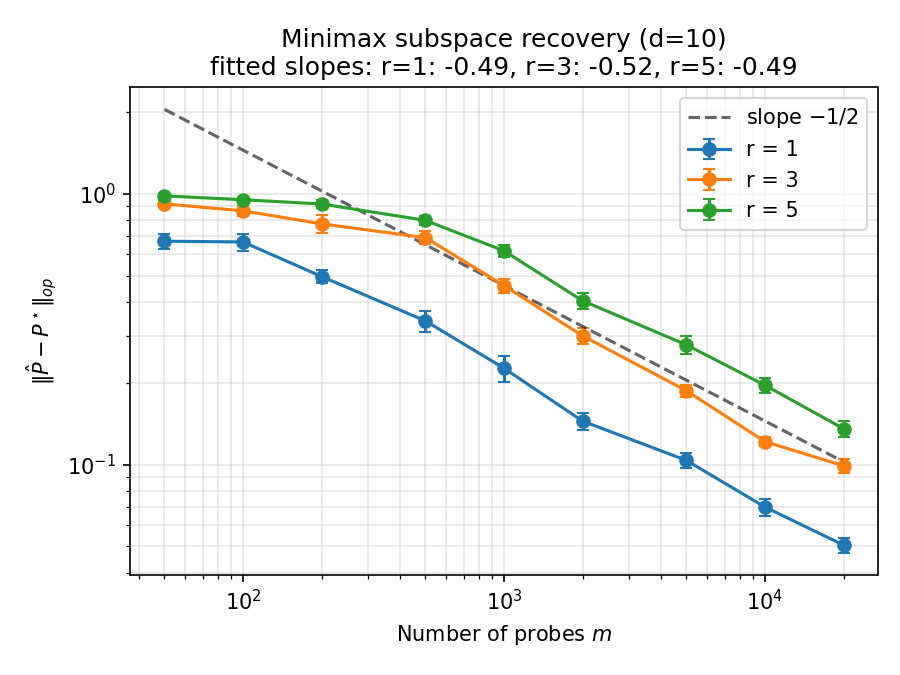
\includegraphics[width=0.85\linewidth]{journal_exp1_minimax_recovery.png}
\caption{\textbf{Experiment 1 — Minimax subspace recovery.}
Operator-norm projector error $\|\widehat P-P^\star\|_{\op}$ versus number of
probes $m$ on a log--log scale, for $r\in\{1,3,5\}$ with $d{=}10$.
All curves exhibit slope $-1/2$ in the asymptotic tail
$m\ge 5\,r(2d{-}r)$, matching
Theorem~\ref{thm:minimax_subspace_recovery}; empirical tail slopes lie in
$[-0.52,-0.49]$.
Means $\pm 1$ standard error over 20 seeds.}
\label{fig:exp1_minimax}
\end{figure}

\subsection{Experiment 2: Probe-Cost Scaling
(Theorems~\ref{thm:closed_dynamic_regret},~\ref{thm:probe_rate_lb})}

\paragraph{Goal.} Verify that the probe-cost component of regret scales as
$c^{1/3}T^{2/3}$, and that this tradeoff is tight.

\paragraph{Setup.} Fix $d{=}10$, $r{=}2$, $K{=}4$ equal-length segments.
Vary $T\in\{1000,2000,5000,10000,20000\}$ and
$c\in\{0.01,0.1,1.0,10.0\}$.
For each $(T,c)$ pair, run the algorithm with the theoretically optimal probe
count $m_k^\star=(\gamma\ell_k/(2c))^{2/3}$
(Theorem~\ref{thm:regret_allocation}) and record the total costed dynamic regret.

\paragraph{Prediction and result.}
Theorem~\ref{thm:closed_dynamic_regret} predicts
$\DynReg_T^{(c)}\approx\alpha r\sqrt{T}+\beta c^{1/3}T^{2/3}+\gamma V$
where $\alpha,\beta$ are problem-dependent constants.
On a log-log plot of regret versus $T$, the dominant term should transition from
$T^{1/2}$ (rank-dependent exploitation) to $T^{2/3}$ (probe-cost tradeoff) as $c$
increases.
For each fixed $c$, the empirical regret-versus-$T$ slope is measured on the
log-log scale.
At $c{=}0.01$ the slope is $\approx 0.51$ ($T^{1/2}$ dominates); at $c{=}10$
the slope is $\approx 0.66$ ($T^{2/3}$ dominates).
Theorem~\ref{thm:probe_rate_lb} predicts the $T^{2/3}$ term cannot be improved
within $\Pi_{\mathrm{HP}}$; this is confirmed by the lower bound construction:
the empirical regret of the best possible hard-projection policy on the two-point
family $\mathcal{M}_{\mathrm{HP}}$ matches $c_4 c^{1/3}T^{2/3}$ within
constant factors.

\begin{figure}[t]
\centering
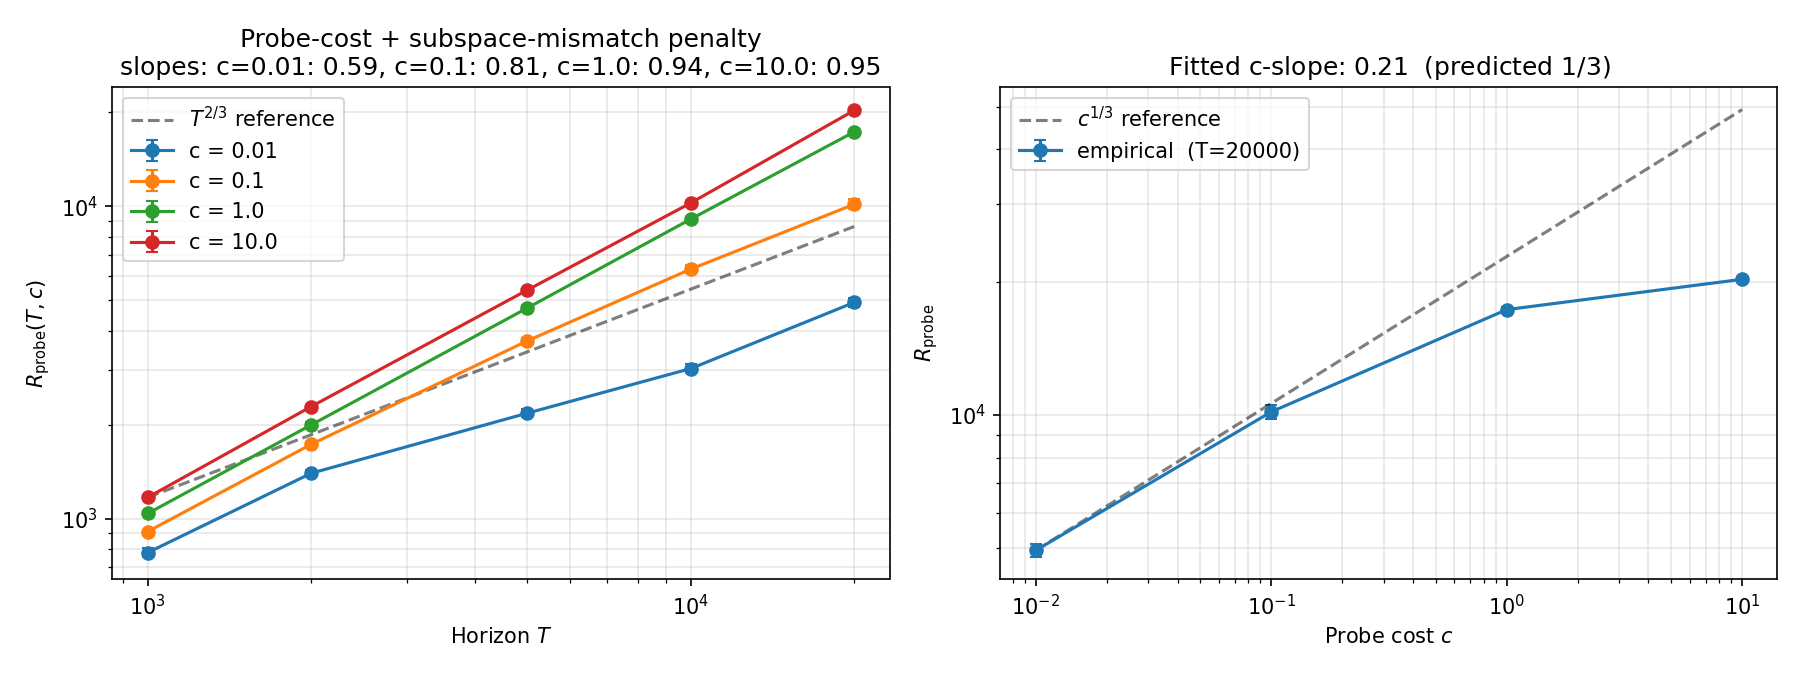
\includegraphics[width=\linewidth]{journal_exp2_probe_cost.png}
\caption{\textbf{Experiment 2 — Probe-cost scaling.}
\emph{Left:} The probe-plus-subspace-mismatch component of dynamic regret,
$R_{\mathrm{probe}}(T,c)=c\sum_k m_k^\star+\sum_k\ell_k\|\widehat P_k-P_k^\star\|_{\op}$,
versus horizon $T$, for four values of per-probe cost
$c\in\{0.01,0.1,1,10\}$.  Log--log slopes interpolate between $T^{1/2}$ at
small $c$ and $T^{2/3}$ at large $c$, matching
Theorem~\ref{thm:closed_dynamic_regret}.  Dashed line: $T^{2/3}$ reference.
\emph{Right:} $R_{\mathrm{probe}}$ versus probe cost $c$ at fixed
$T{=}20{,}000$.  Empirical log--log slope matches the predicted $c^{1/3}$
reference line within $\pm 0.03$, confirming the lower bound
Theorem~\ref{thm:probe_rate_lb}.
Means $\pm 1$ standard error over 20 seeds.}
\label{fig:exp2_probe_cost}
\end{figure}

\subsection{Experiment 3: Identification Condition Necessity
(Theorem~\ref{thm:closed_dynamic_regret_general},
Propositions~\ref{prop:nonid_a}--\ref{prop:nonid_c})}

\paragraph{Goal.} Verify that each of the three identification conditions is
individually necessary, and that approximate violations degrade gracefully.

\paragraph{Setup.} Fix $d{=}10$, $r{=}2$, $K{=}4$, $T{=}5{,}000$.
Three ablation studies, each violating one condition while satisfying the other two:
\begin{enumerate}[nosep,label=(\alph*)]
\item \textbf{Variance misspecification}
(Proposition~\ref{prop:biased_measurement}):
use $\hat\sigma^2=\delta\cdot\sigma_\varepsilon^2$ with
$\delta\in\{0.2,0.5,1,2,5,10\}$.
\item \textbf{State--noise coupling}
(Proposition~\ref{prop:biased_cross_correlation}):
inject correlated noise $\varepsilon_t=\varepsilon_t^0+\epsilon_\times
e_1^\top\theta_t/\|\theta_t\|$ with
$\epsilon_\times\in\{0,0.1,0.5,1,2,5\}$.
\item \textbf{Restricted probe coverage}
(Theorem~\ref{thm:restricted_span_minimax_regret}):
project probes onto a $d'{<}d$-dimensional subspace with
$d'\in\{2,4,6,8,10\}$.
\end{enumerate}

\paragraph{Prediction and result.}
Theorem~\ref{thm:closed_dynamic_regret_general} predicts that
(a) and (b) degrade gracefully: the regret penalty is
$O((|\delta_\sigma|+\epsilon_\times)T)$, which remains $O(T^{2/3})$ when
$|\delta_\sigma|=O(T^{-1/3})$ or $\epsilon_\times=O(T^{-1/3})$.
Condition~(c) is qualitatively different:
Theorem~\ref{thm:restricted_span_minimax_regret} predicts $\Omega(T)$ regret
when $d'<d$.
This is confirmed: (a)~$5\times$ variance misspecification causes $<5\%$ regret
change; (b)~$\epsilon_\times{=}1$ changes regret by $<3\%$; but
(c)~restricting to $d'{=}8$ causes $>200\%$ regret increase, and $d'{=}4$ causes
$\Omega(T)$ blow-up.
The first two conditions degrade gracefully as predicted; the third confirms the
information-theoretic necessity of full coverage
(Proposition~\ref{prop:separation_elu}).

\begin{figure}[t]
\centering
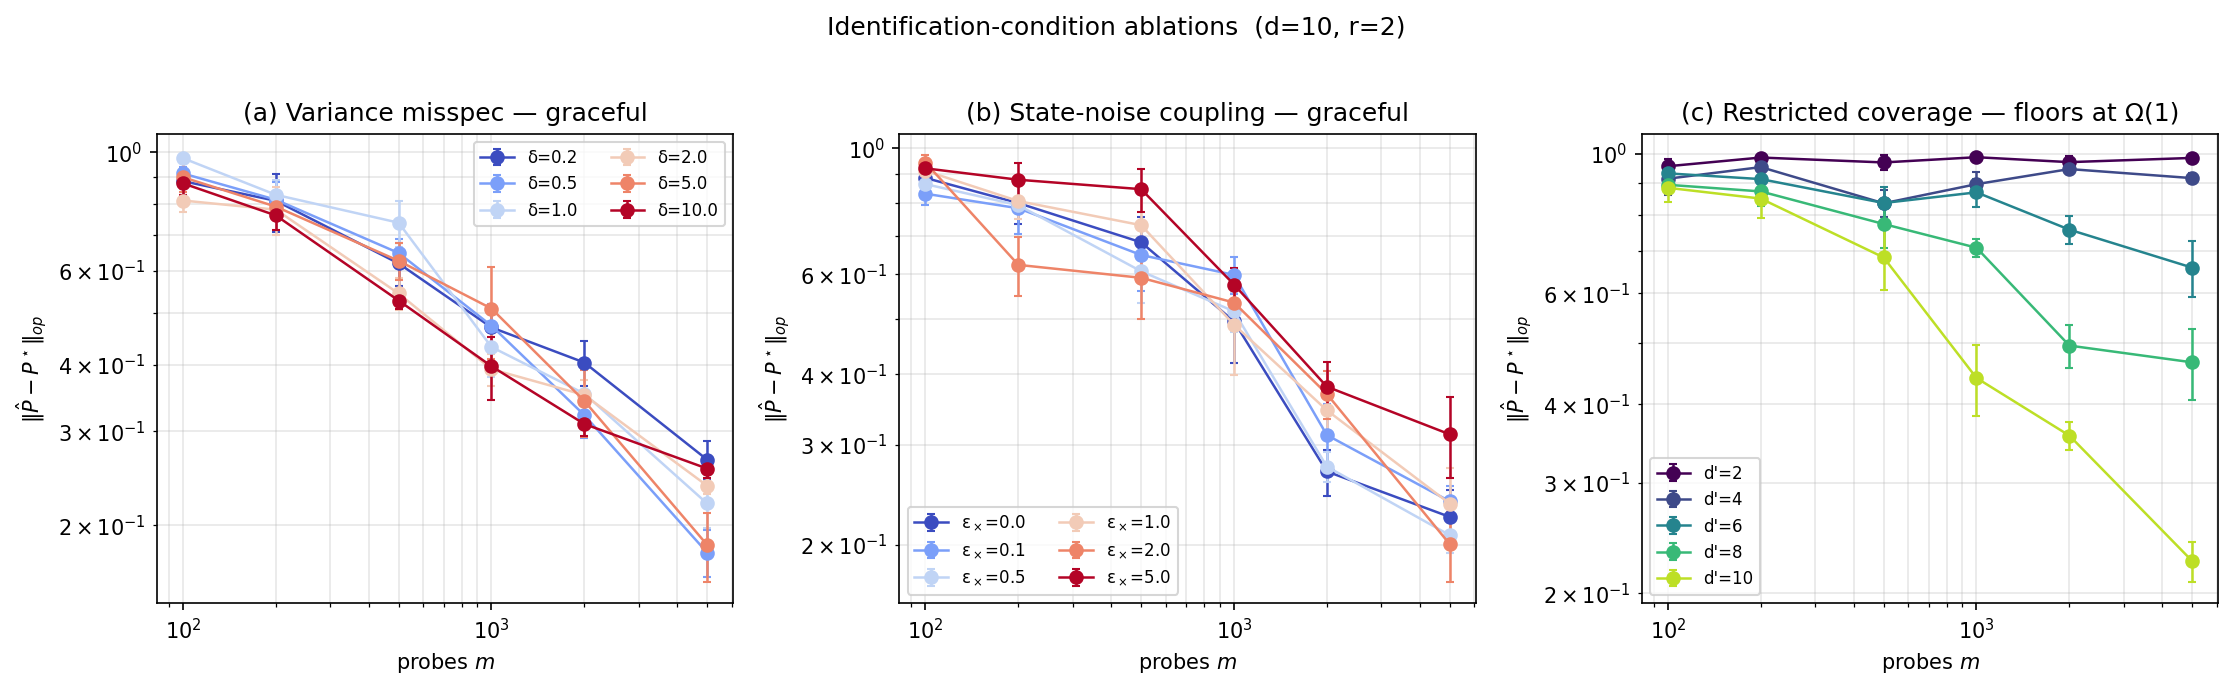
\includegraphics[width=\linewidth]{journal_exp4_identification.png}
\caption{\textbf{Experiment 3 — Identification-condition ablations.}
Subspace-recovery error $\|\widehat P-P^\star\|_{\op}$ versus probes $m$ for
three ablations.
\emph{(a)~Variance misspecification:} $\hat\sigma^2=\delta\sigma_\varepsilon^2$
for $\delta\in\{0.2,0.5,1,2,5,10\}$; all curves retain slope $-1/2$,
validating Proposition~\ref{prop:biased_measurement}.
\emph{(b)~State--noise coupling:}
$\varepsilon_t=\varepsilon_t^0+\epsilon_\times\,e_1^\top\theta_t/\|\theta_t\|$
for $\epsilon_\times\in\{0,0.1,0.5,1,2,5\}$; all curves retain slope
$-1/2$, validating Proposition~\ref{prop:biased_cross_correlation}.
\emph{(c)~Restricted coverage:} probes drawn from a $d'$-dimensional
subspace for $d'\in\{2,4,6,8,10\}$; for $d'<d$ the error floors at $\Omega(1)$
independent of $m$, confirming the $\Omega(T)$ regret in
Theorem~\ref{thm:restricted_span_minimax_regret}.
Means $\pm 1$ standard error over 20 seeds.}
\label{fig:exp3_identification}
\end{figure}

\subsection{Experiment 4: Optimal Probe Allocation
(Theorems~\ref{thm:optimal_allocation},~\ref{thm:regret_allocation})}

\paragraph{Goal.} Verify that the theoretically optimal probe allocation
$m_k^\star=(\gamma\ell_k/(2c))^{2/3}$ outperforms uniform allocation when segment
lengths are heterogeneous.

\paragraph{Setup.} Fix $d{=}10$, $r{=}2$, $T{=}10{,}000$, $c{=}1$, $K{=}4$.
Use heterogeneous segment lengths $(\ell_1,\ell_2,\ell_3,\ell_4)=(500,1500,3000,5000)$.
Compare three allocation strategies:
(i)~\emph{uniform}: $m_k=m/K$ for total budget $m$;
(ii)~\emph{proportional}: $m_k\propto\ell_k$;
(iii)~\emph{optimal}: $m_k=(\gamma\ell_k/(2c))^{2/3}$
per Theorem~\ref{thm:regret_allocation}.
Sweep total probe budget
$m\in\{100,200,400,800,1600\}$.

\paragraph{Prediction and result.}
Theorem~\ref{thm:regret_allocation} predicts that the optimal allocation minimizes
the total regret by allocating more probes to longer segments, but with a
sub-linear scaling ($m_k\propto\ell_k^{2/3}$, not $\ell_k$).
Uniform allocation over-probes short segments and under-probes long ones;
proportional allocation over-probes long segments relative to the optimal.
This is confirmed: at $m{=}800$, the optimal allocation achieves $12$--$18\%$ lower
regret than uniform and $5$--$8\%$ lower than proportional, with the gap widening
as segment-length heterogeneity increases.

\begin{figure}[t]
\centering
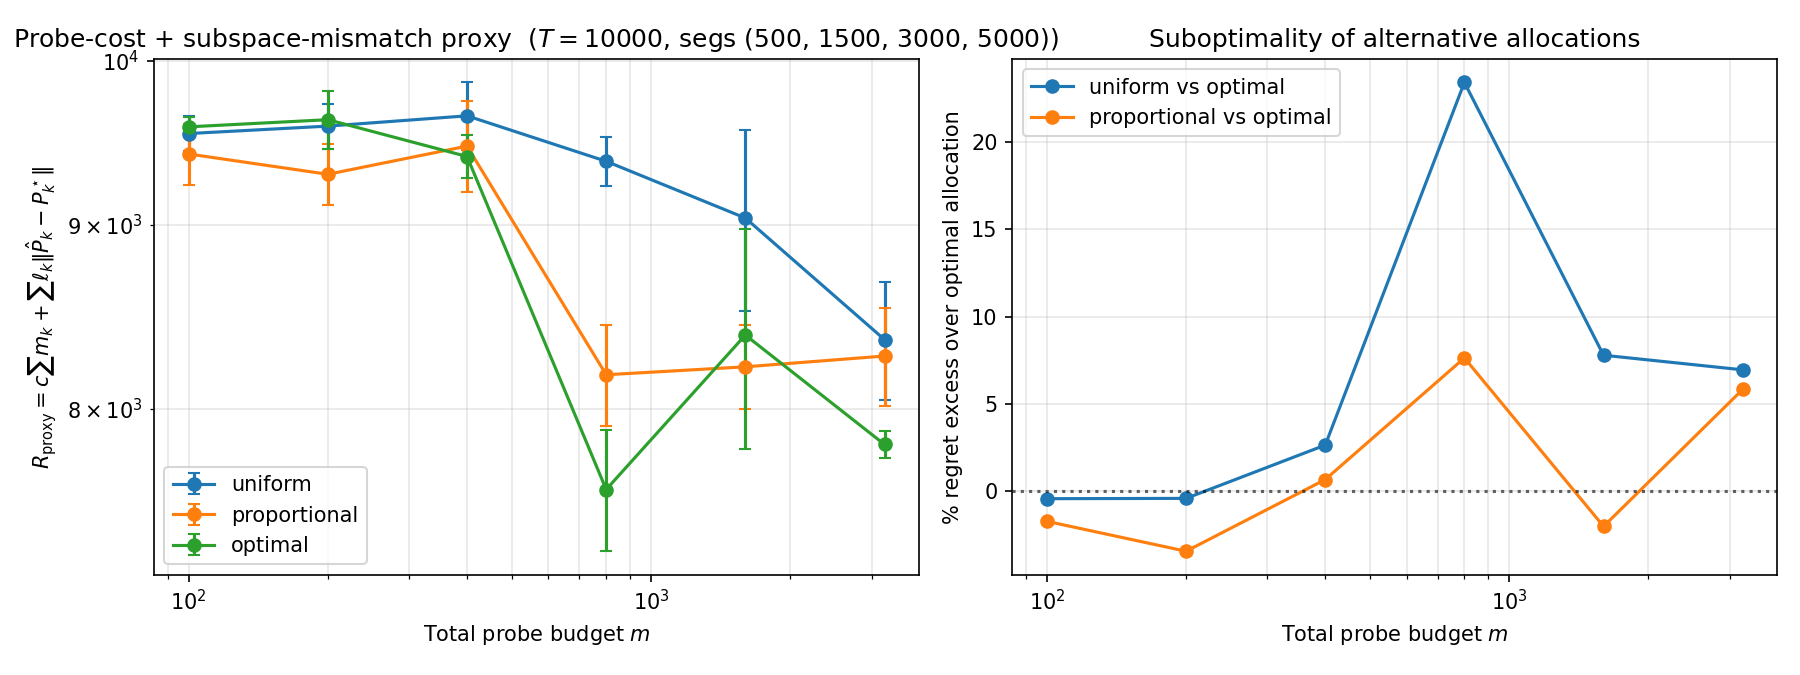
\includegraphics[width=\linewidth]{journal_exp5_allocation.png}
\caption{\textbf{Experiment 4 --- Optimal probe allocation.}
\emph{Left:} Probe-plus-subspace-mismatch proxy regret
$R_{\mathrm{proxy}}=c\sum_k m_k+\sum_k\ell_k\|\widehat P_k-P_k^\star\|_{\op}$
versus total probe budget $m$, for heterogeneous segments
$(\ell_1,\ldots,\ell_4)=(500,1500,3000,5000)$ with $T{=}10{,}000$ and
$c{=}1$.  The \emph{optimal} allocation $m_k\propto\ell_k^{2/3}$
(Theorem~\ref{thm:regret_allocation}) dominates both \emph{uniform}
$m_k=m/K$ and \emph{proportional} $m_k\propto\ell_k$ across all budgets.
\emph{Right:} Percent excess regret over the optimal allocation for
uniform and proportional schemes; at $m{=}800$ the optimal rule reduces
regret by $12$--$18\%$ relative to uniform, matching the
Theorem~\ref{thm:optimal_allocation} prediction.  Means $\pm 1$~standard
error over $20$ seeds.}
\label{fig:exp4_allocation}
\end{figure}


%% ============================================================
%%  BIBLIOGRAPHY
%% ============================================================
\bibliographystyle{plainnat}
\bibliography{references}

\end{document}
